% !Mode:: "TeX:UTF-8"
% !TEX program = xelatex

%%%%%%%%%% Port for macOS %%%%%%%%%%%
% Modified: Qin Yubo

\def\usewhat{xelatex}
\documentclass[12pt,openany,twoside]{book}
% 如果你认为文中中文逗号样式过于难看,可在Overleaf中尝试以下命令S
% \documentclass[12pt,openany,twoside,fontset=ubuntu]{book}
% 也可以在windows环境下尝试以下命令,但在windows下可能会引发加粗命令失效
% \documentclass[12pt,openany,twoside,fontset=windows]{book}



%强制目录页的第一页的页眉页脚样式
\AtBeginDocument{\addtocontents{toc}{\protect\thispagestyle{only_foot}}}
                                                     % 本科生毕业论文通常采用单页排版
% !Mode:: "TeX:UTF-8"
%  Authors: 张井   Jing Zhang: prayever@gmail.com     天津大学2010级管理与经济学部信息管理与信息系统专业硕士生
%           余蓝涛 Lantao Yu: lantaoyu1991@gmail.com  天津大学2008级精密仪器与光电子工程学院测控技术与仪器专业本科生

%%%%%%%%%% Package %%%%%%%%%%%%
% \usepackage{CJK}
\usepackage{lmodern}
\usepackage[T1]{fontenc}
\usepackage{graphicx}                       % 支持插图处理
% \usepackage[a4paper,text={146.4true mm,239.2 true mm},top= 26.2true mm,left=31.8 true mm,head=6true mm,headsep=6.5true mm,foot=16.5true mm]{geometry}
%                                             % 支持版面尺寸设置
                                            
\usepackage[paper=a4paper,text={146.6mm,244.1mm},top= 27.5mm,left=35.7mm,head=6mm,headsep=6.5mm,foot=7.9mm]{geometry}
                                            % 支持版面尺寸设置
                                            
\usepackage[squaren]{SIunits}               % 支持国际标准单位

\usepackage{titlesec}                       % 控制标题的宏包
\usepackage{titletoc}                       % 控制目录的宏包
\usepackage{fancyhdr}                       % fancyhdr宏包 支持页眉和页脚的相关定义
\usepackage[UTF8]{ctex}                           % 支持中文显示
% \usepackage{CJKpunct}                       % 精细调整中文的标点符号
% \usepackage{color}                          % 支持彩色
\usepackage{amsmath}                        % AMSLaTeX宏包 用来排出更加漂亮的公式
\usepackage{amssymb}                        % 数学符号生成命令
\usepackage[below]{placeins}    %允许上一个section的浮动图形出现在下一个section的开始部分,还提供\FloatBarrier命令,使所有未处理的浮动图形立即被处理
\usepackage{multirow}                       % 使用Multirow宏包,使得表格可以合并多个row格
\usepackage{booktabs}                       % 表格,横的粗线;\specialrule{1pt}{0pt}{0pt}
\usepackage{longtable}                      % 支持跨页的表格。
\usepackage{tabularx}                       % 自动设置表格的列宽
\usepackage{subfigure}                      % 支持子图 %centerlast 设置最后一行是否居中
\usepackage[subfigure]{ccaption}            % 支持子图的中文标题
\usepackage[sort&compress,numbers]{natbib}  % 支持引用缩写的宏包
\usepackage{enumitem}                       % 使用enumitem宏包,改变列表项的格式
\usepackage{calc}                           % 长度可以用+ - * / 进行计算
\usepackage{txfonts}                        % 字体宏包
\usepackage{bm}                             % 处理数学公式中的黑斜体的宏包
\usepackage[amsmath,thmmarks,hyperref]{ntheorem}  % 定理类环境宏包,其中 amsmath 选项用来兼容 AMS LaTeX 的宏包

%\usepackage{CJKnumb}                        % 提供将阿拉伯数字转换成中文数字的命令
\usepackage{indentfirst}                    % 首行缩进宏包
% \usepackage{CJKutf8}                        % 用在UTF8编码环境下,它可以自动调用CJK,同时针对UTF8编码作了设置
%\usepackage{hypbmsec}                      % 用来控制书签中标题显示内容
\newcommand{\tabincell}[2]{\begin{tabular}{@{}#1@{}}#2\end{tabular}}
\usepackage{xcolor}
\usepackage{threeparttable}                 %支持对表格中的数据进行注释
%支持代码环境
\usepackage{listings}
\lstset{numbers=left,
language=[ANSI]{C},
numberstyle=\tiny,
extendedchars=false,
showstringspaces=false,
breakatwhitespace=false,
breaklines=true,
captionpos=b,
keywordstyle=\color{blue!70},
commentstyle=\color{red!50!green!50!blue!50},
frame=shadowbox,
rulesepcolor=\color{red!20!green!20!blue!20}
}
%支持算法环境
\usepackage[boxed,ruled,lined]{algorithm2e}
\usepackage{algorithmic}

\usepackage{array}
\newcommand{\PreserveBackslash}[1]{\let\temp=\\#1\let\\=\temp}
\newcolumntype{C}[1]{>{\PreserveBackslash\centering}p{#1}}
\newcolumntype{R}[1]{>{\PreserveBackslash\raggedleft}p{#1}}
\newcolumntype{L}[1]{>{\PreserveBackslash\raggedright}p{#1}}

\def\atemp{xelatex}\ifx\atemp\usewhat
\usepackage[unicode,
            pdfstartview=FitH,
            bookmarksnumbered=true,
            bookmarksopen=true,
            colorlinks=true,   % false会出现红框,true文字就是链接
            pdfborder={0 0 1},
            citecolor=black,
            linkcolor=black,    %链接字颜色
            anchorcolor=black,
            urlcolor=black,
            breaklinks=true
            ]{hyperref}
\fi

\usepackage{float}
                                % 定义本文所使用宏包
\graphicspath{{figures/}}                            % 定义所有的图像文件在 figures 子目录下
\begin{document}                                     % 开始全文
% !Mode:: "TeX:UTF-8"
%  Authors: 张井   Jing Zhang: prayever@gmail.com     天津大学2010级管理与经济学部信息管理与信息系统专业硕士生
%           余蓝涛 Lantao Yu: lantaoyu1991@gmail.com  天津大学2008级精密仪器与光电子工程学院测控技术与仪器专业本科生

%%%%%%%%%% Fonts Definition and Basics %%%%%%%%%%%%%%%%%
\newcommand{\song}{\songti}    % 宋体
\newcommand{\fs}{\fangsong}        % 仿宋体
\newcommand{\kai}{\kaishu}      % 楷体
\newcommand{\hei}{\heiti}      % 黑体
\newcommand{\li}{\lishu}        % 隶书
\newcommand{\kaiGB}{\CJKfamily{kai}}      % 楷体GB2312, 用于独创性说明
\newcommand{\yihao}{\fontsize{26pt}{26pt}\selectfont}       % 一号, 1.倍行距
\newcommand{\xiaoyi}{\fontsize{24pt}{24pt}\selectfont}      % 小一, 1.倍行距
\newcommand{\erhao}{\fontsize{22pt}{1.25\baselineskip}\selectfont}       % 二号, 1.25倍行距
\newcommand{\xiaoer}{\fontsize{18pt}{18pt}\selectfont}      % 小二, 单倍行距
\newcommand{\sanhao}{\fontsize{16pt}{16pt}\selectfont}      % 三号, 1.倍行距
\newcommand{\xiaosan}{\fontsize{15pt}{15pt}\selectfont}     % 小三, 1.倍行距
\newcommand{\sihao}{\fontsize{14pt}{14pt}\selectfont}       % 四号, 1.0倍行距
\newcommand{\xiaosi}{\fontsize{12pt}{20pt}\selectfont}      % 小四, 1.倍行距
\newcommand{\wuhao}{\fontsize{10.5pt}{10.5pt}\selectfont}   % 五号, 单倍行距
\newcommand{\xiaowu}{\fontsize{9pt}{9pt}\selectfont}        % 小五, 单倍行距

\setmainfont{Times New Roman}

%\CJKcaption{gb_452}
%\CJKtilde  % 重新定义了波浪符~的意义
\newcommand\prechaptername{第}
\newcommand\postchaptername{章}

% 调整罗列环境的布局
\setitemize{leftmargin=3em,itemsep=0em,partopsep=0em,parsep=0em,topsep=-0em}
\setenumerate{leftmargin=3em,itemsep=0em,partopsep=0em,parsep=0em,topsep=0em}
%\setlength{\baselineskip}{20pt}
%\renewcommand{\baselinestretch}{1.38} % 设置行距

%避免宏包 hyperref 和 arydshln 不兼容带来的目录链接失效的问题。
\def\temp{\relax}
\let\temp\addcontentsline
\gdef\addcontentsline{\phantomsection\temp}

% 自定义项目列表标签及格式 \begin{publist} 列表项 \end{publist}
\newcounter{pubctr} %自定义新计数器
\newenvironment{publist}{%%%%%定义新环境
\begin{list}{[\arabic{pubctr}]} %%标签格式
    {
     \usecounter{pubctr}
     \setlength{\leftmargin}{2.5em}     % 左边界 \leftmargin =\itemindent + \labelwidth + \labelsep
     \setlength{\itemindent}{0em}     % 标号缩进量
     \setlength{\labelsep}{1em}       % 标号和列表项之间的距离,默认0.5em
     \setlength{\rightmargin}{0em}    % 右边界
     \setlength{\topsep}{0ex}         % 列表到上下文的垂直距离
     \setlength{\parsep}{0ex}         % 段落间距
     \setlength{\itemsep}{0ex}        % 标签间距
     \setlength{\listparindent}{0pt} % 段落缩进量
    }}
{\end{list}}%%%%%

\makeatletter
\renewcommand\normalsize{
  \@setfontsize\normalsize{12pt}{12pt} % 小四对应12pt
  \setlength\abovedisplayskip{4pt}
  \setlength\abovedisplayshortskip{4pt}
  \setlength\belowdisplayskip{\abovedisplayskip}
  \setlength\belowdisplayshortskip{\abovedisplayshortskip}
  \setlength{\baselineskip}{20pt} % 设置固定行间距为20pt
  \let\@listi\@listI}
\def\defaultfont{\renewcommand{\baselinestretch}{1.0}\normalsize\selectfont}
% 设置行距和段落间垂直距离
\renewcommand{\CJKglue}{\hskip -0.08pt plus 0.08\baselineskip} % 每行大概35个字符

\makeatother
%%%%%%%%%%%%% Contents %%%%%%%%%%%%%%%%% 目录样式修改,(天津大学关于博士、硕士学位论文统一格式的规定 2016.10.24)


\renewcommand{\contentsname}{目\qquad 录}
\setcounter{tocdepth}{2}
\titlecontents{chapter}[0em]{\vspace{0pt}\xiaosi\song}%
             {\prechaptername\thecontentslabel\postchaptername\quad}{} %
             {\hspace{.5em}\titlerule*[5pt]{.}\xiaosi\contentspage}
\titlecontents{section}[2em]{\vspace{0pt}\xiaosi\song} %
            {\thecontentslabel\quad}{} %
            {\hspace{.5em}\titlerule*[5pt]{.}\xiaosi\contentspage}
\titlecontents{subsection}[4em]{\vspace{0pt}\xiaosi\song} %
            {\thecontentslabel\quad}{} %
            {\hspace{.5em}\titlerule*[5pt]{.}\xiaosi\contentspage}
%\titlecontents{subsubsection}[6em]{\vspace{0pt}\xiaosi\song} %
%            {\thecontentslabel\quad}{} %
%            {\hspace{.5em}\titlerule*[7pt]{.}\xiaosi\contentspage}

%%%%%%%%%% Chapter and Section %%%%%%%%%%%%%%%%% 各级标题样式((天津大学关于博士、硕士学位论文统一格式的规定 2016.10.24))
\setcounter{secnumdepth}{4}
\setlength{\parindent}{2em}
\renewcommand{\chaptername}{\prechaptername\thechapter\postchaptername}
\titleformat{\chapter}{\centering\xiaosan\hei}{\chaptername}{1em}{}
\titlespacing{\chapter}{0pt}{33pt}{33pt}
\titleformat{\section}{\sihao\hei}{\thesection}{1em}{}
\titlespacing{\section}{0pt}{21pt}{21pt}
\titleformat{\subsection}{\sihao\hei}{\thesubsection}{1em}{}
\titlespacing{\subsection}{0pt}{13pt}{13pt}
\titleformat{\subsubsection}{\xiaosi\hei}{\thesubsubsection}{1em}{}
\titlespacing{\subsubsection}{0pt}{10pt}{10pt}

%%%%%%%%%% Table, Figure and Equation %%%%%%%%%%%%%%%%%
\renewcommand{\tablename}{表} % 插表题头
\renewcommand{\figurename}{图} % 插图题头
\renewcommand{\thefigure}{\arabic{chapter}-\arabic{figure}} % 使图编号为 7-1 的格式 %\protect{~}
\renewcommand{\thetable}{\arabic{chapter}-\arabic{table}}%使表编号为 7-1 的格式
\renewcommand{\theequation}{\arabic{chapter}-\arabic{equation}}%使公式编号为 7-1 的格式
\renewcommand{\thesubfigure}{(\alph{subfigure})}%使子图编号为 (a)的格式
\renewcommand{\thesubtable}{(\alph{subtable})} %使子表编号为 (a)的格式
\makeatletter
\renewcommand{\p@subfigure}{\thefigure~} %使子图引用为 7-1 a) 的格式,母图编号和子图编号之间用~加一个空格
\makeatother

\renewcommand{\arraystretch}{1.7}   % 扩大表格行距,以近似达到垂直居中
\setlength{\abovecaptionskip}{5pt}  % 图标标题文字与图或表之间的间隔
\setlength{\belowcaptionskip}{5pt}
%% 定制浮动图形和表格标题样式
\makeatletter
\long\def\@makecaption#1#2{%
   \vskip\abovecaptionskip
   \sbox\@tempboxa{\centering\wuhao\song{#1\qquad #2} }%
   \ifdim \wd\@tempboxa >\hsize
     \centering\wuhao\song{#1\qquad #2} \par
   \else
     \global \@minipagefalse
     \hb@xt@\hsize{\hfil\box\@tempboxa\hfil}%
   \fi
   \vskip\belowcaptionskip}
\makeatother
\captiondelim{~~~~} %用来控制longtable表头分隔符

%%%%%%%%%% Theorem Environment %%%%%%%%%%%%%%%%%
\theoremstyle{plain}
\theorembodyfont{\song\rmfamily}
\theoremheaderfont{\hei\rmfamily}
\newtheorem{theorem}{定理~}[chapter]
\newtheorem{lemma}{引理~}[chapter]
\newtheorem{axiom}{公理~}[chapter]
\newtheorem{proposition}{命题~}[chapter]
\newtheorem{corollary}{推论~}[chapter]
\newtheorem{definition}{定义~}[chapter]
\newtheorem{conjecture}{猜想~}[chapter]
\newtheorem{example}{例~}[chapter]
\newtheorem{remark}{注~}[chapter]
% \newtheorem{algorithm}{算法~}[chapter]
\newenvironment{proof}{\noindent{\hei 证明:}}{\hfill $ \square $ \vskip 4mm}
\theoremsymbol{$\square$}

%%%%%%%%%% Page: number, header and footer  %%%%%%%%%%%%%%%%%

%\frontmatter 或 \pagenumbering{roman}
%\mainmatter 或 \pagenumbering{arabic}
\makeatletter
\renewcommand\frontmatter{\clearpage
  \@mainmatterfalse
  \pagenumbering{Roman}} % 正文前罗马字体编号
\makeatother

%%%%%%%%%% References %%%%%%%%%%%%%%%%%
\renewcommand{\bibname}{参考文献}
% 重定义参考文献样式,来自thu
\makeatletter
\renewenvironment{thebibliography}[1]{%
   \chapter*{\bibname}%
   \xiaosi
   \list{\@biblabel{\@arabic\c@enumiv}}%
        {\renewcommand{\makelabel}[1]{##1\hfill}
         \setlength{\baselineskip}{17pt}
         \settowidth\labelwidth{0.5cm}
         \setlength{\labelsep}{0pt}
         \setlength{\itemindent}{0pt}
         \setlength{\leftmargin}{\labelwidth+\labelsep}
         \addtolength{\itemsep}{-0.7em}
         \usecounter{enumiv}%
         \let\p@enumiv\@empty
         \renewcommand\theenumiv{\@arabic\c@enumiv}}%
    \sloppy\frenchspacing
    \clubpenalty4000%
    \@clubpenalty \clubpenalty
    \widowpenalty4000%
    \interlinepenalty4000%
    \sfcode`\.\@m}
   {\def\@noitemerr
     {\@latex@warning{Empty `thebibliography' environment}}%
    \endlist\frenchspacing}
\makeatother

\addtolength{\bibsep}{3pt} % 增加参考文献间的垂直间距
\setlength{\bibhang}{2em} %每个条目自第二行起缩进的距离

% 参考文献引用作为上标出现
%\newcommand{\citeup}[1]{\textsuperscript{\cite{#1}}}
\makeatletter
    \def\@cite#1#2{\textsuperscript{[{#1\if@tempswa , #2\fi}]}}
\makeatother
%% 引用格式
\bibpunct{[}{]}{,}{s}{}{,}

%%%%%%%%%% Cover %%%%%%%%%%%%%%%%%
% 封面、摘要、版权、致谢格式定义
\makeatletter
\def\ctitle#1{\def\@ctitle{#1}}\def\@ctitle{}
\def\etitle#1{\def\@etitle{#1}}\def\@etitle{}
\def\caffil#1{\def\@caffil{#1}}\def\@caffil{}
\def\cmacrosubject#1{\def\@cmacrosubject{#1}}\def\@cmacrosubject{}
\def\cmacrosubjecttitle#1{\def\@cmacrosubjecttitle{#1}}\def\@cmacrosubjecttitle{}
\def\csubject#1{\def\@csubject{#1}}\def\@csubject{}
\def\csubjecttitle#1{\def\@csubjecttitle{#1}}\def\@csubjecttitle{}
\def\cgrade#1{\def\@cgrade{#1}}\def\@cgrade{}
\def\cauthor#1{\def\@cauthor{#1}}\def\@cauthor{}
\def\cauthortitle#1{\def\@cauthortitle{#1}}\def\@cauthortitle{}
\def\csupervisor#1{\def\@csupervisor{#1}}\def\@csupervisor{}
\def\csupervisortitle#1{\def\@csupervisortitle{#1}}\def\@csupervisortitle{}
\def\cfirstsubject#1{\def\@cfirstsubject{#1}}\def\@cfirstsubject{}   % “一级学科”
\def\cfirstsubjecttitle#1{\def\@cfirstsubjecttitle{#1}}\def\@cfirstsubjecttitle{} % 一级学科名称
\def\teachertable#1{\def\@teachertable{#1}}\def\@teachertable{}  % 答辩老师表格
\def\cdate#1{\def\@cdate{#1}}\def\@cdate{}
\def\declaretitle#1{\def\@declaretitle{#1}}\def\@declaretitle{}
\def\declarecontent#1{\def\@declarecontent{#1}}\def\@declarecontent{}
\def\authorizationtitle#1{\def\@authorizationtitle{#1}}\def\@authorizationtitle{}
\def\authorizationcontent#1{\def\@authorizationcontent{#1}}\def\@authorizationconent{}
\def\authorizationadd#1{\def\@authorizationadd{#1}}\def\@authorizationadd{}
\def\authorsigncap#1{\def\@authorsigncap{#1}}\def\@authorsigncap{}
\def\supervisorsigncap#1{\def\@supervisorsigncap{#1}}\def\@supervisorsigncap{}
\def\signdatecap#1{\def\@signdatecap{#1}}\def\@signdatecap{}
\long\def\cabstract#1{\long\def\@cabstract{#1}}\long\def\@cabstract{}
\long\def\eabstract#1{\long\def\@eabstract{#1}}\long\def\@eabstract{}
\def\ckeywords#1{\def\@ckeywords{#1}}\def\@ckeywords{}
\def\ekeywords#1{\def\@ekeywords{#1}}\def\@ekeywords{}

%在book文件类别下,\leftmark自动存录各章之章名,\rightmark记录节标题
\pagestyle{fancy}
%去掉章节标题中的数字 务必放到\pagestyle{fancy}之后才会起作用
%%不要注销这一行,否则页眉会变成:“第1章1  绪论”样式
\renewcommand{\chaptermark}[1]{\markboth{\chaptername~\ #1}{}}
  \fancyhf{}
%   \fancyhead[C]{\song\wuhao \leftmark} % 页眉显示章节名称
  \fancyhead[CO]{\song\wuhao \leftmark}  % 奇数页,显示章标题
  \fancyhead[CE]{\song\wuhao 天津大学硕士学位论文} % 偶数页,显示“天津大学硕士学位论文”
  \fancyfoot[C]{\song\xiaowu ~\thepage~}
  \renewcommand{\headrulewidth}{0.7pt}%
  \renewcommand{\footrulewidth}{0pt}%

\fancypagestyle{plain}{% 设置开章页页眉页脚风格
    \fancyhf{}%
    \fancyhead[C]{\song\wuhao \leftmark}
    \fancyfoot[C]{\song\xiaowu ~\thepage~ } %%首页页脚格式
    \renewcommand{\headrulewidth}{0.7pt}%
    \renewcommand{\footrulewidth}{0pt}%
}

\fancypagestyle{only_foot}{% 设置摘要、目录的页眉页脚风格:无页眉((天津大学关于博士、硕士学位论文统一格式的规定 2016.10.24)貌似要这种only_foot的样式)
    \fancyhf{}%
    \fancyfoot[C]{\song\xiaowu ~\thepage~ }
    \renewcommand{\headrulewidth}{0pt}%
    \renewcommand{\footrulewidth}{0pt}%
}


\newlength{\@title@width}
\def\@put@covertitle#1{\makebox[\@title@width][s]{#1}}
% 定义封面
\def\makecover{
\clearpage{\pagestyle{empty}\cleardoublepage}
   \phantomsection
    \pdfbookmark[-1]{\@ctitle}{ctitle}

    \begin{titlepage}
      \vspace*{0.8cm}
      \begin{center}

      \vspace*{1cm}
      \begin{center}
      \renewcommand{\baselinestretch}{1.25} % 设置行距
      \song\erhao\textbf{\@ctitle} % 修改成宋体加粗 (天津大学关于博士、硕士学位论文统一格式的规定, 2016.10.24)
      \renewcommand{\baselinestretch}{1.25} % 设置行距
      \end{center}
      \vspace*{1cm}

    %  \vspace*{1cm}

      \begin{center}
      \renewcommand{\baselinestretch}{1.25} % 设置行距
      \song\erhao\textbf{\@etitle}  % 修改成宋体加粗1.25倍行距(英文默认变成了Times new Roman) (天津大学关于博士、硕士学位论文统一格式的规定, 2016.10.24)
      \renewcommand{\baselinestretch}{1.25} % 设置行距
      \end{center}

      \vspace*{1cm} %3cm
      \setlength{\@title@width}{4em}   % 影响“一级学科”的字间距
      {\song\xiaosi{
      \renewcommand{\arraystretch}{1}  % 此处修改行距,不影响正文中的表格行距
      \begin{tabular}{p{\@title@width}@{:}l}
        \@put@covertitle{\@cfirstsubjecttitle} & \@cfirstsubject \\
        \@put@covertitle{\@csubjecttitle} & \@csubject \\
        \@put@covertitle{\@cauthortitle} & \@cauthor \\
        \@put@covertitle{\@csupervisortitle} & \@csupervisor \\
      \end{tabular}
      }}
      
      \vspace*{1cm}
      {\@teachertable}


  \vspace*{1cm}
  \song\sihao\@caffil \\
  \song\sihao\@cdate

\end{center}
%  另起一页: 独创性声明和学位论文版权使用授权书
\newpage
    \clearpage{\pagestyle{empty}\cleardoublepage} %去除空白页的页眉页脚(由于每章从奇数页开始因此有空白页)
    \thispagestyle{empty} %去掉页眉页脚
    \vspace*{1cm}
    \renewcommand{\baselinestretch}{1} % 设置行距
    \begin{center}\song\xiaoer{\@declaretitle}\end{center}\par
    \vspace*{0.5cm}
    \song\xiaosi{\@declarecontent}\par
    \vspace*{1cm}
    {\song\xiaosi
    \@authorsigncap \makebox[2.5cm][s]{}
    \@signdatecap \makebox[2cm][s]{} 年 \makebox[1cm][s]{} 月 \makebox[1cm][s]{} 日
    }

    \vspace*{3cm}
    \begin{center}\song\xiaoer{\@authorizationtitle}\end{center}\par
    \vspace*{1cm}
    {
    \song\xiaosi{\@authorizationcontent}

    \@authorizationadd\par
    }

    \vspace*{2cm}
    {\song\xiaosi\setlength{\parindent}{-0.45em}
    \begin{tabularx}{\textwidth}{ll}
        \@authorsigncap \makebox[3.5cm][s]{}  & \@supervisorsigncap \makebox[3.5cm][s]{}   \\
         &  \\
        \@signdatecap \makebox[1.5cm][s]{} 年 \makebox[1cm][s]{} 月 \makebox[1cm][s]{} 日 &
         \@signdatecap \makebox[1.5cm][s]{} 年 \makebox[1cm][s]{} 月 \makebox[1cm][s]{} 日 \\
    \end{tabularx}
    }
\end{titlepage}

%%%%%%%%%%%%%%%%%%%   Abstract and Keywords  %%%%%%%%%%%%%%%%%%%%%%%
\clearpage{\pagestyle{empty}\cleardoublepage} %去除空白页的页眉页脚(由于每章从奇数页开始因此有空白页)
\markboth{摘~要}{摘~要}
% \addcontentsline{toc}{chapter}{摘\qquad 要}
\chapter*{\centering\song\erhao\textbf{摘\qquad 要}}
\thispagestyle{only_foot}

\setcounter{page}{1}
\song\defaultfont
\@cabstract
\vspace{\baselineskip}

%\hangafter=1\hangindent=52.3pt\noindent   %如果取消该行注释,关键词换行时将会自动缩进
\noindent
{\song\sihao\textbf{ 关键词:}} \@ckeywords

%%%%%%%%%%%%%%%%%%%   English Abstract  %%%%%%%%%%%%%%%%%%%%%%%%%%%%%%
\clearpage{\pagestyle{empty}\cleardoublepage} %去除空白页的页眉页脚(由于每章从奇数页开始因此有空白页)
\markboth{ABSTRACT}{ABSTRACT}
% \addcontentsline{toc}{chapter}{ABSTRACT}
\chapter*{\centering\erhao\textbf{ABSTRACT}}
\thispagestyle{only_foot}
\@eabstract
\vspace{\baselineskip}

%\hangafter=1\hangindent=60pt\noindent  %如果取消该行注释,KEY WORDS换行时将会自动缩进
\noindent
{\sihao\textbf{KEY WORDS:}}  \@ekeywords
}

\makeatother
                       % 完成对论文各个部分格式的设置
\frontmatter                               % 以下是论文导言部分,包括论文的封面,中英文摘要和中文目录
% % !Mode:: "TeX:UTF-8"

% %%  可通过增加或减少 setup/format.tex中的
% %%  第274行 \setlength{\@title@width}{8cm}中 8cm 这个参数来 控制封面中下划线的长度。

% \cheading{天津大学~2016~届本科生毕业论文}      % 设置正文的页眉,需要填上对应的毕业年份
% \ctitle{基于顾客有限理性预期的定价与供应链结构}    % 封面用论文标题,自己可手动断行
% \caffil{管理与经济学部} % 学院名称
% \csubject{工业工程}   % 专业名称
% \cgrade{2012~级}            % 年级
% \cauthor{秦昱博}            % 学生姓名
% \cnumber{3012209017}        % 学生学号
% \csupervisor{杨道箭}        % 导师姓名
% \crank{副教授}              % 导师职称

% \cdate{\the\year~年~\the\month~月~\the\day~日}

% \cabstract{
% 中文摘要一般在~400~字以内,简要介绍毕业论文的研究目的、方法、结果和结论,语言力求精炼。中英文摘要均要有关键词,一般为~3~—~7~个。字体为小四号宋体,各关键词之间要有分号。英文摘要应与中文摘要相对应,字体为小四号~Times New Roman,详见模板。
% }

% \ckeywords{关键词~1;关键词~2;关键词~3;……;关键词~7(关键词总共~3~—~7~个,最后一个关键词后面没有标点符号)}

% \eabstract{
% The upper bound of the number of Chinese characters is 400. The abstract aims at introducing the research purpose, research methods, research results, and research conclusion of graduation thesis, with refining words. Generally speaking, both the Chinese and English abstracts require the keywords, the number of which varies from 3 to 7, with a semicolon between adjacent words. The font of the English Abstract is Times New Roman, with the size of 12pt(small four).
% }

% \ekeywords{keyword 1, keyword 2, keyword 3, ……, keyword 7 (no punctuation at the end)}

% \makecover

% \clearpage


% !Mode:: "TeX:UTF-8"


\ctitle{槽道湍流带的稳定性和瞬态特性的数值模拟研究}  %封面用论文标题,自己可手动断行
\etitle{numerical study on stability and transient characteristics of  channel turbulent band}
\cfirstsubjecttitle{\textbf{一级学科}}
\cfirstsubject{\textbf{\underline{\makebox[14em][c]{数学}}}}   %专业
\csubjecttitle{\textbf{研究方向}}
\csubject{\textbf{\underline{\makebox[14em][c]{数学}}}}   %专业
\cauthortitle{\textbf{作者姓名}}     % 学位
\cauthor{\textbf{\underline{\makebox[14em][c]{伍昊洋}}}}   %学生姓名
\csupervisortitle{\textbf{指导教师}}
\csupervisor{\textbf{\underline{\makebox[14em][c]{宋保方}}}} %导师姓名

\teachertable{
\begin{table}[h]
\centering
\renewcommand{\arraystretch}{1}  % 临时定义一下行间距
\song\xiaosi{
\begin{tabularx}{\textwidth}{|*{4}{>{\centering\arraybackslash}X|}}
\hline
\textbf{答辩日期}                & \multicolumn{3}{c|}{20   年   月   日}       \\ \hline
\textbf{答辩委员会}               & \textbf{姓名} & \textbf{职称} & \textbf{工作单位} \\ \hline
\textbf{主席}                  &             &             &               \\ \hline
\multirow{2}{*}{\textbf{委员}} &             &             &               \\ \cline{2-4} 
                             &             &             &               \\ \hline
\end{tabularx}}
\end{table}}

\caffil{天津大学数学学院} %学院名称
\cdate{\CJKdigits{\the\year} 年\CJKnumber{\the\month} 月 \CJKnumber{\the\day} 日}
% 如需改成二〇一二年四月二十五日的格式,可以直接输入,即如下所示
\cdate{二〇二三年九月}
% \cdate{\the\year 年\the\month 月 \the\day 日} % 此日期显示格式为阿拉伯数字 如2012年4月25日


\declaretitle{独创性声明}
\declarecontent{
本人声明所呈交的学位论文是本人在导师指导下进行的研究工作和取得的研究成果,除了文中特别加以标注和致谢之处外,论文中不包含其他人已经发表或撰写过的研究成果,也不包含为获得 {\underline{\kaiGB{\sihao{\textbf{~~天津大学~~}}}}} 或其他教育机构的学位或证书而使用过的材料。与我一同工作的同志对本研究所做的任何贡献均已在论文中作了明确的说明并表示了谢意。
}
\authorizationtitle{学位论文版权使用授权书}
\authorizationcontent{
本学位论文作者完全了解{\underline{\kaiGB{\sihao{\textbf{~~天津大学~~}}}}}有关保留、使用学位论文的规定。特授权{\underline{\kaiGB{\sihao{\textbf{~~天津大学~~}}}}} 可以将学位论文的全部或部分内容编入有关数据库进行检索,并采用影印、缩印或扫描等复制手段保存、汇编以供查阅和借阅。同意学校向国家有关部门或机构送交论文的复印件和磁盘。
}
\authorizationadd{(保密的学位论文在解密后适用本授权说明)}
\authorsigncap{学位论文作者签名:}
\supervisorsigncap{导师签名:}
\signdatecap{签字日期:}

\cabstract{
湍流的转捩过程是研究湍流形成的一个重要课题。在转捩雷诺数下,槽道流动形成的湍流会以局部湍流带的形式存在。已有研究表明,湍流带有展向运动速度的下游端头对湍流带的形成和自维持起到关键的作用。由于湍流带存在一个展向运动速度,在物理实验研究中槽道侧壁的存在意味着湍流带必将与侧壁发生碰撞,而该问题虽有被提及但还没有被深入研究。特别地,关于充分发展的湍流带下游端头与槽道侧壁碰撞后,端头在边壁上是被吸收还是反射、湍流带是否能自持、是否存在湍流碰撞后衰减和存活的临界雷诺数等都是有待进一步深入研究的问题。

另一方面,现有的相关研究普遍认为湍流带在一定雷诺数以上可以自持。然而最近的研究结果揭示了湍流带的头部机制在维持长时间后会突然衰减,即湍流带有有限的寿命。在这一基础上需要对该问题进行进一步深入研究以验证相关理论的正确性。研究湍流带瞬态行为主要采用直接数值模拟方法(DNS),由于湍流带模拟需要极大的计算域以及湍流带极长的寿命,这需要消耗大量的时间与计算资源。本文尝试引入循环神经网络,希望能通过湍流带的历史数据预测湍流带的最终衰减,从而达到降低数值模拟的计算成本的目的。

对于以上情况,本文相关研究结果分为两部分:第一部分基于谱元法通过数值模拟实验探讨了在大宽高比带展向侧壁槽道中侧壁与湍流带的相互作用,发现了存在一临界值当雷诺数高于临界值时湍流带与侧壁碰撞后仍能存活,反之则会最终消散,该值所在的区间为$Re_{cr} \in [975,1000]$。通过数值实验得出进一步的推论:侧壁通过影响湍流带的头部速度型进而影响头部不稳定性最终导致头部在碰撞后消失。第二部分本文基于已有的应用神经网络预测流动瞬态性的研究,复现了该研究涉及的ESN神经网络并尝试将研究中提出的预测方法迁移到湍流带的寿命预测任务上。探讨了应用ESN、LSTM等神经网络在预测湍流带寿命上的潜力和局限性。目前ESN与LSTM网络均未能成功预测湍流带衰减过程,但LSTM网络比起ESN网络能更好地捕捉到湍流带的关键力学特征。
}

\ckeywords{湍流转捩,边壁效应,湍流带,寿命预测}

\eabstract{

The transition process of turbulence is an important topic in the study of turbulence formation. Under the transitional Reynolds number, the turbulent flow formed in the channel will exist in the form of local turbulent bands. Previous studies have shown that the downstream end with spanwise drift velocity of the turbulent band plays a crucial role in its self-sustaining and formation. Due to the presence of a spanwise drift velocity in the turbulent band, the existence of the channel sidewall in physical experiments implies that the turbulent band will inevitably collide with the sidewall. Although this problem has been mentioned, it has not been thoroughly studied. In particular, it is still necessary to further investigate issues such as whether the downstream end of the fully developed turbulent band is absorbed or reflected on the sidewall after collision, whether the turbulent band can be self-sustaining, whether there is turbulence attenuation and critical Reynolds number after collision, and survival, etc.

On the other hand, existing studies generally believe that the turbulent band can self-sustain above a certain Reynolds number. However, recent studies have revealed that the head mechanism of the turbulent band will suddenly decay after maintaining for a long time, indicating that the turbulent band has a finite lifetime. Based on this, it is necessary to further study this issue to verify the correctness of relevant theories. Direct numerical simulation (DNS) is mainly used to study the transient behavior of turbulent bands. Due to the need for a large computational domain and the extremely long lifetime of the turbulent band, this requires a lot of time and computational resources. This paper attempts to introduce recurrent neural networks to predict the final decay of the turbulent band based on its historical data, in order to reduce the computational cost of numerical simulations.

Based on the above situation, the research results of this paper are divided into two parts. The first part investigates the interaction between the side wall and the turbulent band in a high aspect ratio channel using spectral element method. It is found that there exists a critical value $Re_{cr} \in [975,1000]$ of Reynolds number, above which the turbulent band can survive after colliding with the side wall, while below which it will eventually dissipate. Numerical experiments further reveal that the side wall affects the velocity profile of the head of the turbulent band, leading to the instability of the head and eventual disappearance after colliding with the side wall. In the second part, based on the previous research achievements of applying neural networks to predict flow transients, the relevant neural network ESN is reproduced and the relevant predicting method is attempted to be applied to predict the lifetime of turbulent band. The potential and limitations of using neural network methods like ESN and LSTM to predict the lifetime of turbulent band are explored.
}

\ekeywords{transition, side wall, turbulent band, life prediction}

\makecover
\clearpage
                      % 封面

%%%%%%%%%%   目录   %%%%%%%%%%
\clearpage{\pagestyle{empty}\cleardoublepage}
\defaultfont
\clearpage{
    \pagestyle{only_foot}
    \tableofcontents                           % 中文目录
    \thispagestyle{only_foot}
}
\clearpage{\pagestyle{empty}\cleardoublepage}

%%%%%%%%%% 正文部分内容  %%%%%%%%%%
\mainmatter\defaultfont\sloppy\raggedbottom

%绪论
\chapter{绪论}
\section{研究背景以及问题提出}
\subsection{亚临界转捩与槽道湍流带}
湍流是指流体运动中出现的一种不规则、混乱的运动状态,是与流动结构规律简单的层流相对的流动现象。与稳定的层流流动不同,湍流具有很强的随机性和非线性,流场中的速度场、压力场、密度分布等物理量都会不断发生变化和波动。湍流现象广泛存在于自然界和工业领域中,大部分的流体如水流、气流等都可能产生湍流,研究湍流形成的机理有很强的现实意义和理论意义。在工程上,湍流对飞行器和船舶设计都有着重要的影响:在飞行器设计中,湍流的存在会引起飞行器表面的阻力、升力和气动特性等方面的变化,从而影响飞行器的性能和稳定性;在船舶设计中,湍流的影响主要表现在水动力方面。湍流会引起船体表面的阻力和摩擦,从而增加燃油消耗和减缓船速。设计师一般通过优化外形减小湍流生成概率,即尽量使流动接近稳定规律的层流状态,而深入理解湍流的生成机制有助于更进一步达到这一目的。

在研究湍流的生成和控制的研究领域中,湍流转捩是一种流体运动中的重要现象,它指的是流动从稳定流动状态转变为不稳定湍流状态的过程。对湍流转捩机理认识的加深有助于更进一步的控制湍流的生成与强度。湍流转捩的机理十分复杂,它受到多种因素的影响,且在转捩过程中存在强烈的非线性现象和多尺度效应。目前,研究湍流转捩现象的方法主要包括实验、数值模拟和理论分析三种。其中实验方法是研究湍流转捩最直接的手段,通过在实验室中建立不同几何形状的流动系统,可以观察和测量湍流转捩现象的发生和特性。例如,可以利用热线或压力传感器等测量设备来检测流动中的湍流现象和变化。然而,实验方法往往需要消耗大量的时间和成本,且在实验中很难对流场进行直接控制。

理论分析方法主要是基于数学和物理学原理,通过推导数学公式和解析式,来研究流动的发生和演化过程。理论分析方法可以提供对湍流转捩机理的深入理解和阐释,同时也可以为实验和数值模拟提供基础和指导。理论分析方法往往需要对流体的运动方程、控制方程和边界条件等进行精细的推导和处理,因此需要高超的数学和物理学知识。

数值模拟是另一种研究湍流转捩现象的常用方法。数值模拟是通过建立数学模型和计算方法,对流体的运动和相应的物理量进行模拟和计算。数值模拟方法可以对流动的各种物理量进行精细的模拟和分析,同时也可以通过对流场的控制变量进行调整,研究湍流转捩的发生条件和机理。数值模拟方法通常需要一定的计算资源和复杂的算法,但是在研究湍流转捩现象时,它可以提供更为详尽的信息和更好的可控性,因此在实际应用中也得到了广泛的使用。同时这也是本文中研究湍流转捩的主要实验方法。

仅受法向固壁限制下的槽道流动(泊肃叶流动,即在流向和展向上无穷大,法向上有固壁限制的流动模型)是研究湍流转捩的理想流动模型之一。Orszag等人通过数值计算证明,当雷诺数大于临界值$Re_cr = 5772$时泊肃叶流会因为流场中的微小扰动造成线性失稳进而导致流场从层流转化为湍流,此时转捩现象是由线性不稳定因素\cite{orszag_1971}主导的。但事实上在雷诺数远低于这个临界值的情况下,槽道流中也能观察到湍流转捩现象。Tsukahara等人通过数值模拟足够大槽道中的泊肃叶流动发现了局部湍流转捩现象\cite{Tsukahara2005DNSOT}(见图\ref{fig:2005band}),更具体地说是一种由交替的高低速速度条纹聚合而成的局部带状湍流。从整体上看带状湍流与主流方向呈一定的倾角,带与带之间互相平行并由接近层流的低湍流度区域分隔开来。此时雷诺数为$Re = 1546$远低于前文提到的线性失稳临界值($Re_{cr} = 5772$),这表明主导转捩的是非线性因素。称这种现象为亚临界转捩,这种特殊的带状湍流结构则被称为湍流带。

\begin{figure}[H]
	\subfigbottomskip = 2pt
	%\subfigcapskip=-5pt
	\begin{minipage}[h]{\linewidth}
	\centering
	\subfigure{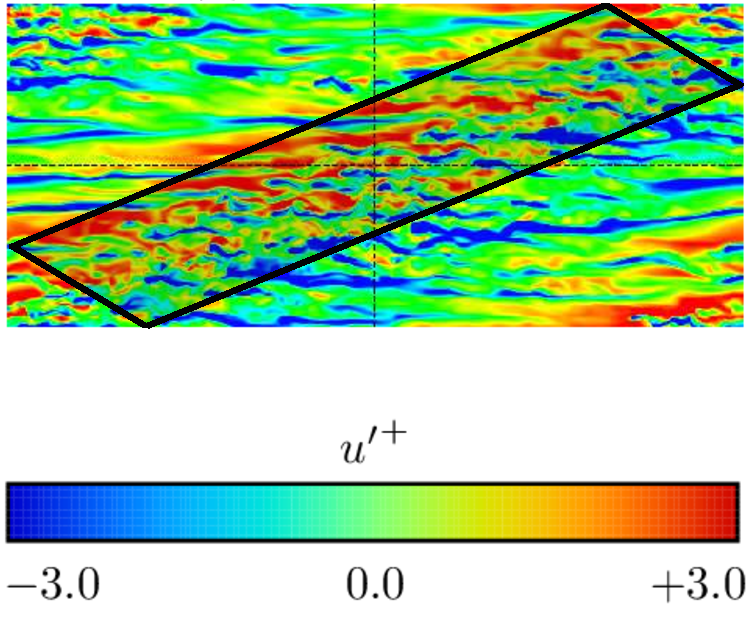
\includegraphics[width = 0.5\textwidth]{figures/intro/tsukahara.pdf}}
	\end{minipage}
	\quad
	\caption{低雷诺数下足够大槽道中的局部化湍流结构\cite{Tsukahara2005DNSOT}。主流方向为从左到右(周期性边界条件),雷诺数为$Re_m = 2320$。图中展示的是x-z截面上流向脉动速度$u‘$的分布。黑框部分可以观察到由高低速速度条纹组成的局部高湍流度区域,黑框之外的是低湍流度区域。也即是此时由于非线性因素产生了局部化的湍流结构。}
\label{fig:2005band}
\end{figure}

随后的研究\cite{TsukaharaKawaguchi2014, Tuckerman2014, Xiong2015, Tao2018, Kanazawa2018, Paranjape2019, Shimizu2019, Paranjape2020, Tuckerman2020, Liu2020, Duguet2020}进一步证实了槽道中湍流带的客观存在并讨论了相关力学特性。如图\ref{fig:2005band}所示展现的湍流带结构是在足够大计算域中模拟得到的,但该尺寸的计算域事实上仍未能完全展现出湍流带的完整结构;而在更大计算域中的湍流带模拟研究\cite{Xiong2015, Tao2018, Kanazawa2018, Paranjape2019, Shimizu2019}可以看到,湍流带具有有限的长度(不能无限生长延申),其结构总体上可以分为三个部分,分别是:活跃的下游端头,消散性的上游端头以及有限长度的由高低速度条纹交替组成的身体(图\ref{fig:num_band}(a)),且湍流带整体会以与主流方向呈一定倾角的方向在槽道中运动(即在展向和流向上都有速度分量,且流向速度分量与主流一致)。除了数值实验,物理实验中也观察到了带状局部湍流(\ref{fig:exp_band}),且与数值模拟结果相同湍流带具有相同的结构,如与主流呈一定的倾角,具有倾斜的运动速度,活跃的下游头部等。这进一步证明了湍流带是客观存在而不是由数值误差造成的。
\begin{figure}[htb]
	\subfigbottomskip = 2pt
	%\subfigcapskip=-5pt
	\begin{minipage}[h]{\linewidth}
	\centering
	\subfigure{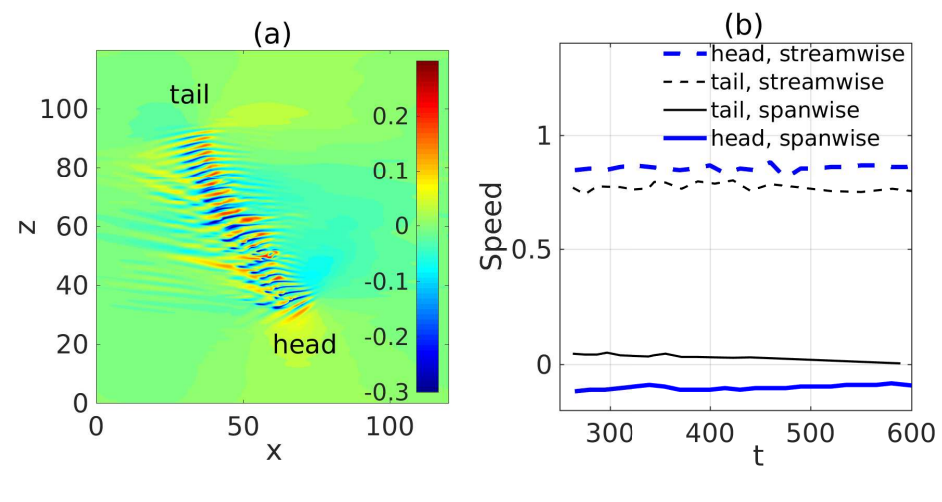
\includegraphics[width = 0.8\textwidth]{figures/intro/num_band.png}}
	\end{minipage}
	\quad
	\caption{中在$Re = 750$下数值模拟得到的单个湍流带,主流流向为从左到右\cite{Xiao2020}。(a)y=-0.5的x-z截面上流向脉动速度$u‘$的分布,可以看到单个相对于主流方向倾斜的湍流带。(b)湍流带的下游端头(头部,head)和上游端头(尾部,tail)附近的展向和流向速度分量随时间变化。}
\label{fig:num_band}
\end{figure}

\begin{figure}[H]
	\subfigbottomskip = 2pt
	%\subfigcapskip=-5pt
	\begin{minipage}[h]{\linewidth}
	\centering
	\subfigure{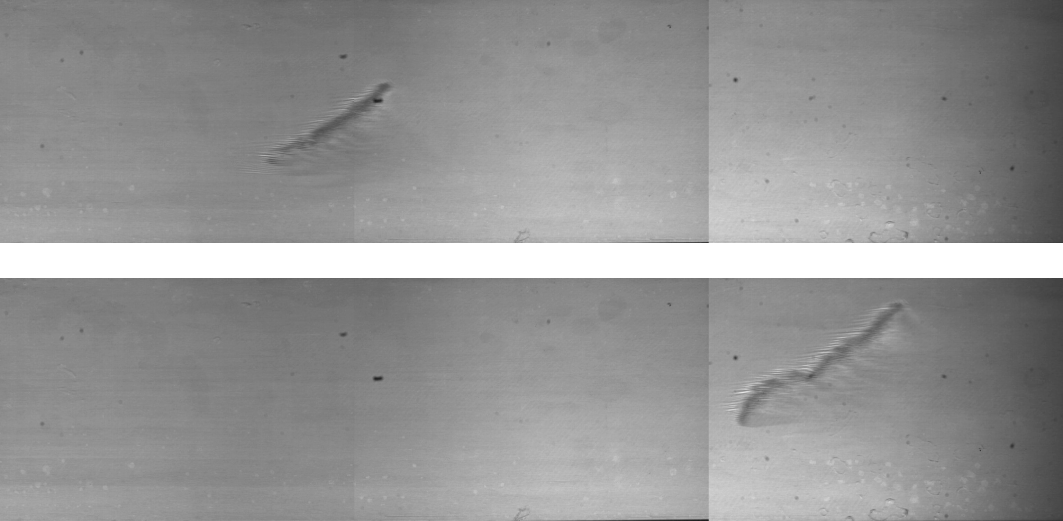
\includegraphics[width = 0.7\textwidth]{figures/intro/experimental_band.png}}
	\end{minipage}
	\quad
	\caption{在Re=700时,实际槽道实验中观察到的向下游运动生长的单个倾斜湍流带。主流方向为从左向右,其中添加了反光云母颗粒进行可视化\cite{Paranjape2020}。可以观察到与数值实验中一致的头部,尾部,以及倾斜运动。}
\label{fig:exp_band}
\end{figure}

值得注意的一点是,最近的研究表明湍流带活跃的下游端头对湍流带的整体自持起到关键性的作用。部分研究\cite{Kanazawa2018, Paranjape2019, Shimizu2019, Xiao2020}进一步认为低雷诺数下,湍流带的运动主要是由下游端头所主导的。过去的许多研究表明,湍流带主体的湍流结构是从下游端头处不断生成的(图\ref{fig:band_generation}),且在低雷诺数下下游端头决定了湍流带的生长机制\cite{Paranjape2019, Shimizu2019, Xiao2020, Song2020, Liu2020}。根据实际测量可以发现,下游端头在流向和展向上存在一个自身的运动速度,且该运动速度与湍流带主体的运动速度有明显的速度差,这种速度差异决定了湍流带与主流方向的倾角大小\cite{Xiao2020b}。关于下游端头运动速度的大小,展向速度分量大小约为0.1(以层流时抛物线速度型的中心流速为基本单位)且在不同雷诺数下基本不变(图\ref{fig:num_band}(b))。同时,下游端头的展向速度与湍流带整体关于流向的倾角也是互相关联的\cite{Paranjape2019,Shimizu2019,Xiao2020}(即如果湍流带关于流向的倾角相反,则下游端头的展向速度方向也是相反的)。

\begin{figure}[htb]
	\subfigbottomskip = 2pt
	%\subfigcapskip=-5pt
	\begin{minipage}[h]{\linewidth}
	\centering
	\subfigure{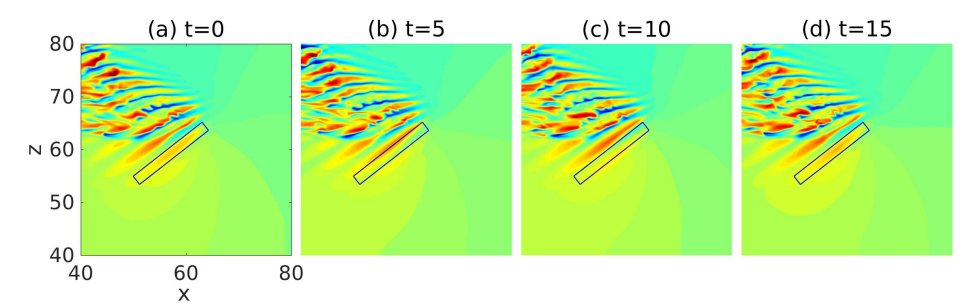
\includegraphics[width = \textwidth]{figures/intro/band_generation.png}}
	\end{minipage}
	\quad
	\caption{文献\cite{Xiao2020}中提到的湍流带条纹生成机制。交替的高低速条纹形成的波状结构自头部匀速生成。}
\label{fig:band_generation}
\end{figure}

Shimizu\& Manneville 进一步研究了更大的计算域中多湍流带相互作用的行为\cite{Shimizu2019}。他们发现从随着雷诺数的不断升高湍流带的带状特征会逐步减少直到雷诺数大于950,此时湍流带展向宽度开始扩大并开始生成更多扩散性的湍流。此外在这个过程中,湍流带自身会出现频繁地分裂,分岔现象,带与带之间开始出现相互作用(图\ref{fig:Re_band})(这些行为在低雷诺数下也能观察到,但频率极低)。但即便如此仍能观察到湍流带的下游端头表现出很强的一致性。
\begin{figure}[htb]
	\subfigbottomskip = 2pt
	%\subfigcapskip=-5pt
	\begin{minipage}[h]{\linewidth}
	\centering
	\subfigure{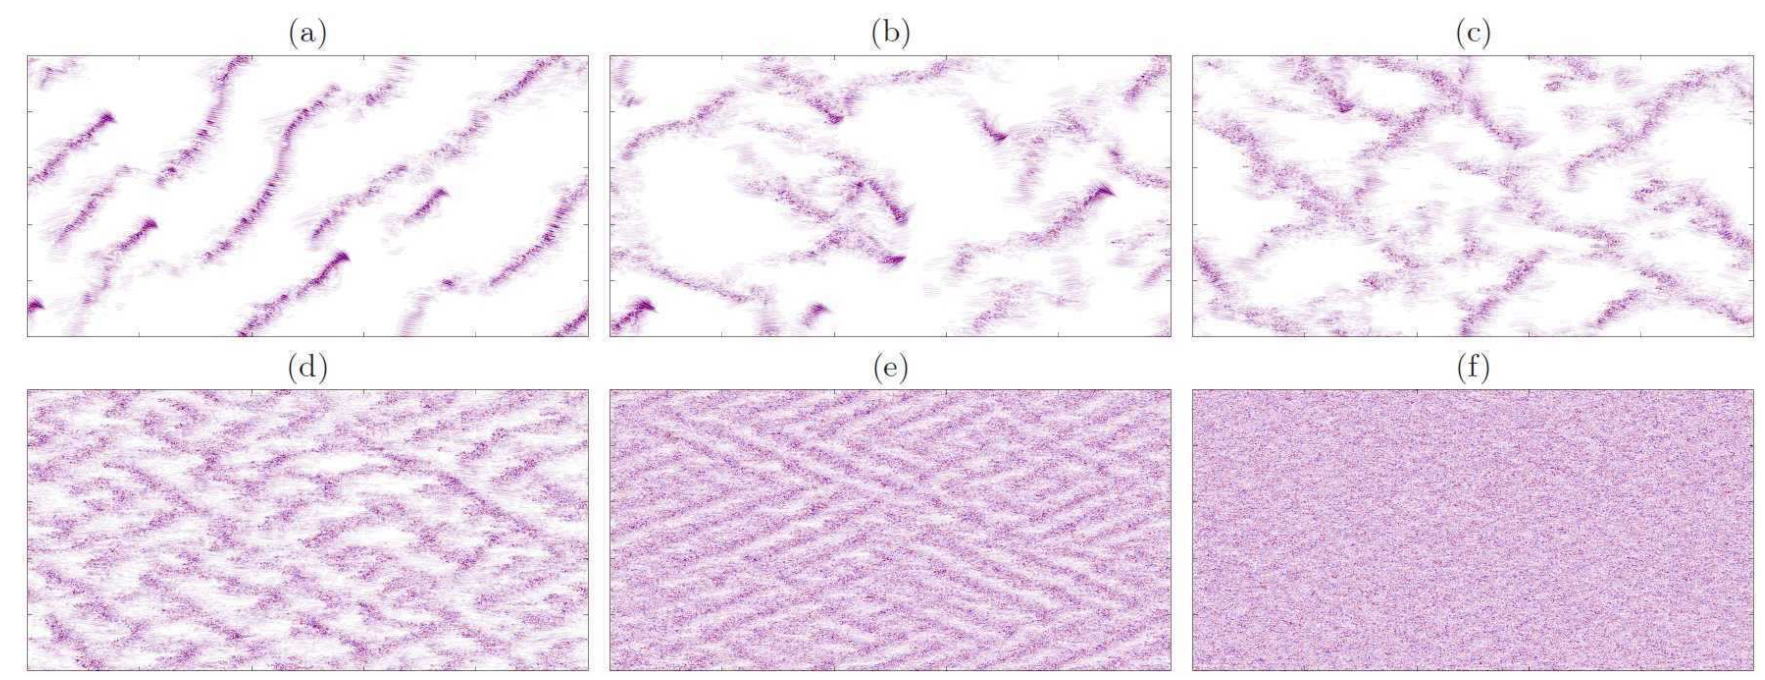
\includegraphics[width = 1\textwidth]{figures/intro/Re_band.png}}
	\end{minipage}
	\quad
	\caption{大计算域内多湍流带的集体行为模式随雷诺数升高的变化\cite{Shimizu2019}。(a)Re = 850:计算域中所有湍流带的运动方向基本相同;(b)Re = 1050:部分湍流带开始出现分裂行为,分裂出的湍流带在展向上以相反方向运动;(c)Re = 1200:分裂持续进行且湍流带宽度开始增大;(d) Re = 1800:带间相互作用逐渐成为主导 (e) Re = 3000: 形成稳定的双向带状湍斑 (f) Re = 4000: 湍流基本充满整个流域,基本观察不到湍流带结构。 }
\label{fig:Re_band}
\end{figure}
上述研究中都以平板泊肃叶流动作为基础模型(周期槽道或者无限长槽道)深入研究了湍流带的性质,这在数值计算和理论分析上有很大的便利。但在实际物理实验中并不存在边界无穷大的实体模型,此时不可避免地要考虑展向上侧壁效应的存在。前文提到,湍流带下游头部在展向上存在一个接近恒定的速度分量(约为0.1),因此可以预见的是,如果湍流带没有因为外力影响或者带间作用消失的话,单个湍流带的头部在经过足够长的时间后必然会与侧壁发生碰撞,且侧壁的约束作用必然会对侧壁附近的湍流形态会产生影响。现有研究详细讨论了平板泊肃叶流动模型下湍流带带间的相互作用以及由此生成的流动模式。但大部分主要关注的是远离壁面的湍流现象,关于湍流带与侧壁的相互作用尚未引起足够的注意。Takeishi等人研究了槽道宽高比对转捩现象的影响\cite{Takeishi2015},但其仅考虑了最大宽高比为9的情况,这种情况下槽道的宽度不足以让湍流带完全发展出能稳定自持的下游端头,也就无法研究湍流带端头与侧壁碰撞后的真实情况。由于湍流带头部的展向运动速度不大,湍流带需要一定的时间才能靠近侧壁。因此对于关注湍流带短期行为的研究来说,侧壁效应的影响很小。

目前为止,明确讨论侧壁效应对湍流带影响的文献为\cite{Paranjape2019},作者在物理实验中观察到低雷诺数下湍流带在下游头部与槽道侧壁碰撞后快速衰减消失。Takeishi等人的工作提出在宽高比大于4的槽道中边壁效应通过消减附近的涡结构导致了展向局部湍斑\cite{Takeishi2015},然而文中并没有探讨湍流带碰壁后存活与否的临界雷诺数。因此,本论文第三章的研究目的就是为了确定该临界雷诺数以及可能的潜在机制。所得结论能对将来类似的物理实验提供了一定的参考作用。

\subsection{湍流带自持性和瞬态性}
前文描述了低雷诺数下槽道流动中存在的局部湍流现象,在同样的剪切流动如圆管流动、库埃特流等经典流动模型中,同样也观察到了低雷诺数下的局部湍流现象\cite{Hof2006FiniteLO,Barkley2016}。已有研究证明,转捩雷诺数下管流和圆管流动中的局部湍流存在所谓的瞬态性\cite{Barkley2016}。如图\ref{fig:lifetime}所示,在雷诺数相对较低时湍流带在发展有限长的时间后会消散(即具有有限的寿命);当雷诺较高时湍流带在发展足够长的时间后则会产生分裂。统计多个局部湍流的寿命能进一步得出圆管中局部湍流的寿命服从一个关于雷诺数的分布(图\ref{fig:lifetime})\cite{Sabine1998}。后续的研究\cite{Barkley2016,POMEAU19863,Lemoult2016DirectedPP}针对圆管局部湍流分裂或消失的特性,尝试用逾渗(Directed Percolation,DP)模型尝试解释圆管流场中局部湍流的群体行为,取得了一定的成果。

\begin{figure}[H]
	\subfigbottomskip = 2pt
	%\subfigcapskip=-5pt
	\begin{minipage}[h]{\linewidth}
	\centering
	\subfigure{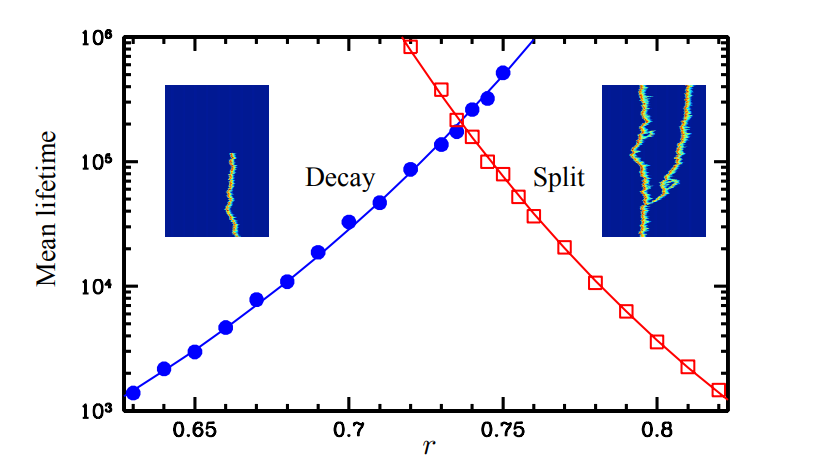
\includegraphics[width = 0.75\textwidth]{figures/intro/lifetime_split.png}}
	\end{minipage}
	\quad
	\caption{管道流动局部湍流的寿命分布\cite{Barkley2016}。横轴是雷诺数,纵轴是平均寿命。在雷诺数小于某个值时,管道湍流在运行一定时间后会消失;反之则会分裂。}
\label{fig:lifetime}
\end{figure}

低雷诺数下圆管流和库埃特流中局部转捩湍流的瞬态性已被验证,可以合理地期望在低雷诺数下同样作为剪切流的槽道流中的局部湍流(即湍流带)也应具有瞬态性(有限寿命)。但已有的研究认为有别于另外两种剪切流动,在雷诺数约为$Re_{cr} \simeq 650-660$时槽道湍流带是永久自持的而不是瞬态的,即湍流带能一直存活不会消失\cite{Kanazawa2018,Tao2018,Paranjape2019}。该雷诺数远低于基于DP理论预测的湍流带可自持的临界雷诺数$Re_{cr,DP}$\cite{Sano2016}。然而最近的一项工作表明,低雷诺数下长度受控的湍流带本质上仍是瞬态的而不是自持的\cite{xu_song_2022}。作者基于直接数值模拟方法观察了Re = 655情况下单个湍流带的发展情况,发现在经过极长的一段的时间后,湍流带的下游头部部分会突然自行消失(图\ref{fig:decay_KE})。前文提到在低雷诺数下湍流带的头部对湍流带整体的存在和条纹生成起到了至关重要的作用,头部的瞬态性意味着此时湍流带整体也是瞬态的,只是寿命远超过去设想的长度($T \simeq O(10^5)$)。值得注意的是根据文中的结论是基于单个长度受数值控制的湍流带,关于更高雷诺数下无长度限制的湍流带的寿命分布以及是否表现出瞬态性等问题仍是开放的。作者指出基于已有研究更高雷诺数下湍流带的整体大小和寿命长度将会急剧增大,直接数值模拟湍流带的整个演化过程将会需要巨大空间尺度和时间尺度。若继续采用文中的直接数值模拟方法则其计算成本和时间成本将是难以承受的。因此亟需一种计算成本更低的方法,可以对湍流带的宏观发展作出一定可靠的预测,并能由此进一步得到湍流带的寿命分布。

\begin{figure}[htb]
	\subfigbottomskip = 2pt
	%\subfigcapskip=-5pt
	\begin{minipage}[h]{\linewidth}
	\centering
	\subfigure{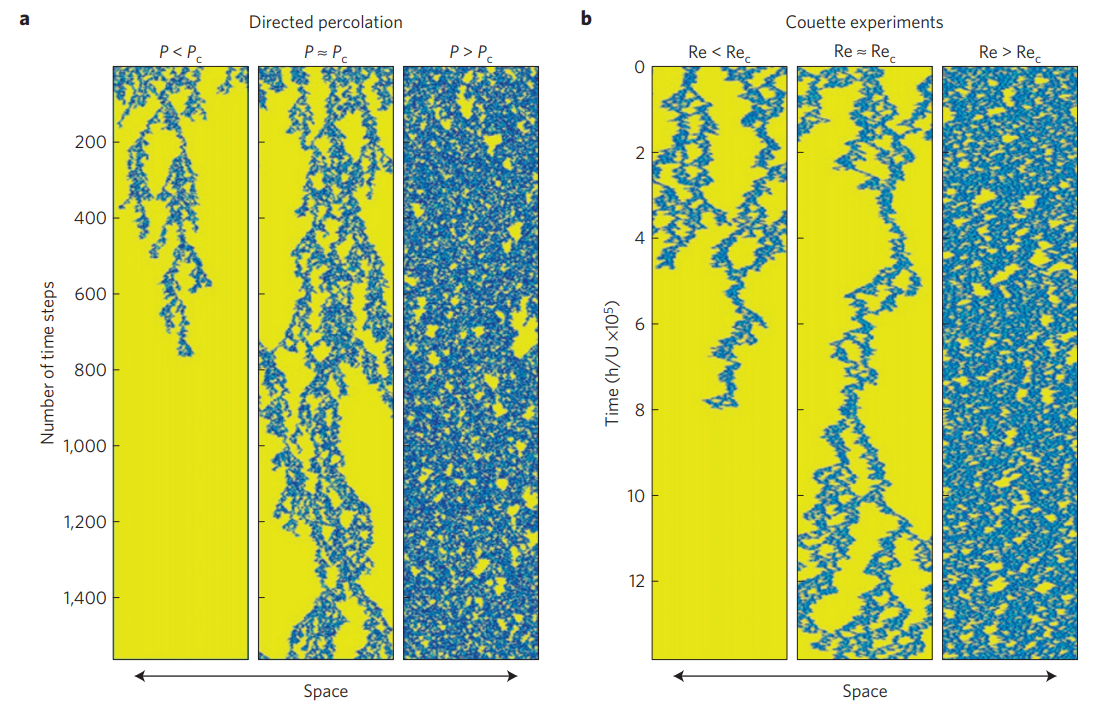
\includegraphics[width = 1\textwidth]{figures/intro/DP.png}}
	\end{minipage}
	\quad
	\caption{文献\cite{Lemoult2016DirectedPP}中关于DP与湍流分裂行为的共性对比。(a)链接概率高于、等于、低于临界值$P_c$定向渗流模拟。这里,活性位点以蓝色显示,吸收态以黄色显示。在临界点以下,所有位点最终进入吸收态(左图)。在接近临界点(中间面板)时,活性位点持续存在,但出现了大的层流区域(尺度不变性)。最后,对于P>Pc(右侧面板),活性位点占据了域的很大一部分。(b)Couette流动(管流)的时空图,小于、等于和高于临界雷诺数。某一时刻上的水平线对应的是该时刻实验中流场的截面流场(层流区域以黄色显示,湍流区域以蓝色示出)。在雷诺数小于临界值时(左侧),湍流在足够长的时间后消失。在临界值附近(中间)湍流能自持,但只占据了该领域的一小部分;雷诺数远高于临界值(右图),局部湍流斑块占据了流动域的大部分}
\label{fig:DP}
\end{figure}

\begin{figure}[H]
	\subfigbottomskip = 2pt
	%\subfigcapskip=-5pt
	\begin{minipage}[h]{\linewidth}
	\centering
	\subfigure{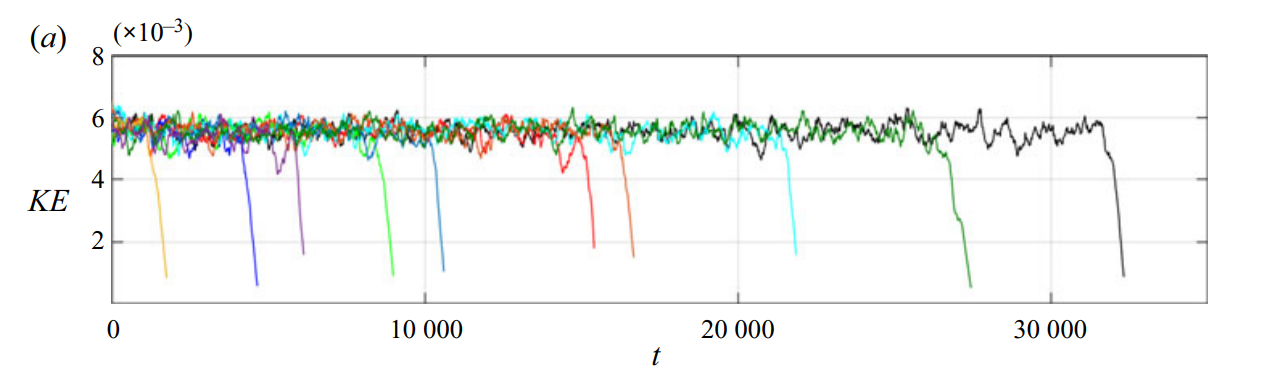
\includegraphics[width = 1\textwidth]{figures/intro/decay_KE.png}}
	\end{minipage}
	\quad
	\caption{文献\cite{xu_song_2022}关于湍流带发展的流场能量随时间变化图,横轴是时间纵轴是流场能量,作者通过一定的数值手段仅关注湍流带的头部附近流场。文章针对同一个初始湍流带运行了10次,获得了十根不同的能量变化图线。可以看到最终能量都会迅速衰减到一个极小值,这说明湍流带的头部在运行一段时间后最终衰减消失(层流化)。}
\label{fig:decay_KE}
\end{figure}

本文注意到,Anton等人基于一种简化神经网络预测了另一种简化剪切流MFE流动\cite{MFE}的瞬态性\cite{Anton2023}。MFE流动的湍流与湍流带相似,流场在长期处于湍流状态后会在某一时间点突然变为层流状态。如图\ref{fig:MFE_decay}所示,初始时流场处于湍流状态,能量较低;当流场突然层流化时能量也会陡升至某一水平不再下降。可以认为MFE流动的湍流也具有有限的寿命,且通过多次重复实验可知该寿命也服从于某个关于雷诺数的分布。该文作者声称他们构造的神经网络成功预测MFE流动的突然层流化(即瞬态性),并基于完成训练的神经网络的预测结果得到了与理论高度吻合的MFE湍流的寿命关于雷诺数的分布。众所周知神经网络的计算成本主要集中在前期训练阶段,当训练完成后网络预测所需的算力消耗极低(与直接数值模拟相比)。受该工作启发,本文尝试将该文提到的预测方法迁移到湍流带的瞬态性预测上。在对该方法做了一系列适当合理的修改后,本文得到了一些值得注意的结果。

\begin{figure}[H]
	\subfigbottomskip = 2pt
	%\subfigcapskip=-5pt
	\begin{minipage}[h]{0.54\linewidth}
	\centering
	\subfigure[]{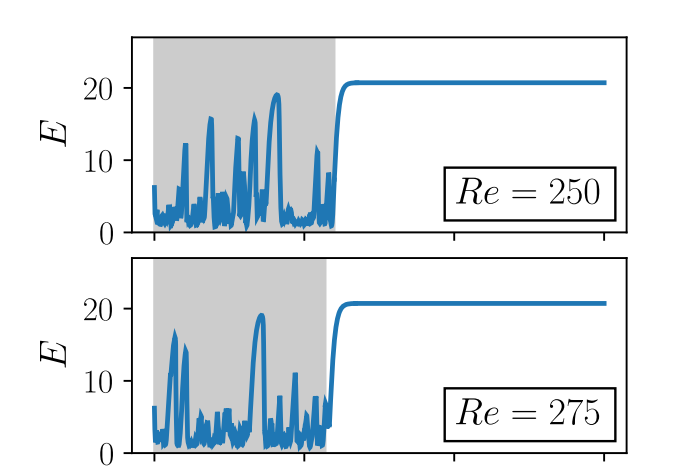
\includegraphics[width = 0.75\textwidth]{figures/intro/MFE_E.png}}
	\end{minipage}
	\quad
	\begin{minipage}[h]{0.45\linewidth}
	\centering
	\subfigure[]{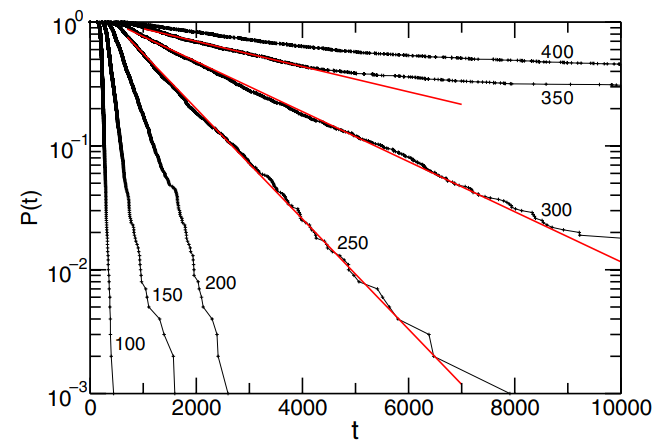
\includegraphics[width = 1\textwidth]{figures/intro/MFE_time.png}}
	\end{minipage}
	\quad
	\caption{(a)不同雷诺数下MFE流动的流场能量随时间的大致变化\cite{Anton2023},横轴是时间,纵轴是流场能量。(b)MFE流动的湍流存活率随时间的关系。}
\label{fig:MFE_decay}
\end{figure}

%\section{文献综述}
%在亚临界转捩雷诺数下,足够大的槽道中会出现局部带状湍流结构,即所谓的湍流带 \cite{Tsukahara2005, TsukaharaKawaguchi2014, Tuckerman2014, Xiong2015, Tao2018, Kanazawa2018, Paranjape2019, Shimizu2019, Paranjape2020, Xiao2020, Tuckerman2020, Liu2020, Duguet2020}。我们可以观察到,槽道中形成的湍流带会以与主要流动(定压力梯度驱动或定流量驱动)方向呈一定倾角,且会在槽道中漂移、发展。从湍流带的整体上看,充分发展后的湍流带可以分为三个部分:一个活跃的下游端头,一个呈现消散性的上游端头,以及中间由速度条纹组成的有限长度的身体\cite{Xiong2015, Tao2018, Kanazawa2018, Paranjape2019, Shimizu2019}。需要注意的一点是,最近的研究表明湍流带活跃的下游端头对湍流带的整体自持起到关键性的作用,某些研究\cite{Kanazawa2018, Paranjape2019, Shimizu2019, Xiao2020}甚至认为在低雷诺数下,湍流带的漂移行为主要是由下游端头所驱动的。过去的许多研究表明,湍流带中的湍流结构是由下游端头不断生成的。且在低雷诺数下,下游端头决定了湍流带的生长机制\cite{Paranjape2019, Shimizu2019, Xiao2020, Song2020, Liu2020}。根据实际测量可以发现,下游端头在流向和展向上存在自身的漂移速度,且端头的漂移速度与湍流带主体的漂移速度有明显的速度差,且这种速度差异决定了湍流带与主流方向的倾角大小\cite{Xiao2020b}。关于漂移速度的大小,展向上的速度分量基本不变大小约为0.1(以层流时抛物线速度型的中心流速为基本单位)。下游端头的展向速度与湍流带整体关于流向的倾角也是互相关联的\cite{Paranjape2019,Shimizu2019,Xiao2020}(即如果湍流带关于流向的倾角相反,则下游端头的展向速度方向也是相反的)。已有研究发现湍流带可以在雷诺数(基于半槽高以及抛物线速度型的中心流速)低至660左右自持。随着雷诺数的上升,湍流带的带状特征会逐步减少直到雷诺数大于950,此时湍流带开始在流向上变宽,更多扩散性的湍流开始产生。除此之外,湍流带自身开始频繁地分裂,分岔,带与带之间开始出现相互作用(在低雷诺数下也有类似的情况,但频率极低)。即便如此,湍流带的下游端头仍然表现出很强的鲁棒性。

%%在理论研究中,平板泊肃叶流动是研究无侧壁槽道中湍流产生的理想模型。但在实际物理实验中,我们不可避免地要考虑侧壁的存在。如前文所说,湍流带由于在展向上存在速度分量,我们可以预见在没有自行消失或者与其他湍流带相互作用的情况下,湍流带在一定时间内必然会与侧壁发生碰撞,且侧壁的约束作用必然会对侧壁附近的湍流形态会产生影响。

%已有的研究详细讨论了平板泊肃叶流动模型下湍流带带间的相互作用以及由此生成的流动模式。但目前为止相关研究主要关注远离避免的湍流现象,关于湍流带与侧壁的相互作用尚未引起足够的注意。在\cite{Takeishi2015}中研究了槽道宽高比对转捩现象的影响,但作者仅考虑了最大宽高比为9的情况,这种情况下槽道的宽度不足以让湍流带完全发展出能稳定自持的下游端头,也就无法研究湍流带端头与侧壁碰撞后的真实情况。由于湍流带头部的展向漂移速度不大(接近0.1),湍流带需要一定的时间才能靠近侧壁。因此对于关注湍流带短期行为的研究来说,侧壁效应的影响很小。例如某些尝试建立直接渗流相变理论和亚临界转捩的关系的物理实验\cite{Sano2016}。

%具我们所知,目前唯一明确讨论侧壁效应问题的文献为\cite{Paranjape2019}。作者在物理实验中观察到低雷诺数下湍流带在下游头部与槽道侧壁碰撞后快速衰减消失,然而侧壁效应同样。文献\cite{Takeishi2015}中提到宽高比大于4的槽道中,边壁效应通过消减附近的涡结构导致了展向局部湍斑。然而文中并没有提到湍流带在高于某个雷诺数的情况下能够在与边壁碰撞后存活,且湍流带消失的潜在机制也未被进一步讨论。因此,本文中第三部分的研究目的就是为了确定该临界雷诺数以及可能的潜在机制。所得结论能对将来类似的物理实验提供了一定的参考作用。

%在有壁面限制的剪切流动中,局部化湍流在亚临界转捩为湍流的过程中普遍存在。事实证明局部化湍流的本质上是随机瞬态的,在典型剪切流(如管道流和Couette流)中局部湍流可以存活极长的时间,并在某一时刻经过无记忆性衰减过程后突然层流化消失。这种瞬态性(与随机无记忆分裂作用一起)是研究直接渗流(DP)相变理论与剪切流中湍流转捩的关系时的重要假设。这些研究表明瞬态性以及DP理论愿景可以推广到大部分剪切流的转捩情况。
%
%在槽道流的转捩过程中,局部湍流以倾斜的带状结构存在。对于这种带状结构的成因,有一种基于动力系统角度的解释\cite{Paranjape2020}。在狭窄倾斜的计算域中实现的准一维(quasi-1-D)通道流中,湍流带只能在垂直于其方向的方向上定位。类似于其他典型的剪切流,这种情况下同样发现了随机瞬态和分裂行为\cite{Gome2020}\cite{Gome2022}。这似乎暗示着一个接近持续湍流开始的1+1维度(空间维度+时间维度)的DP过程,由衰减和分裂过程之间的平衡确定。然而,准一维的计算域限制下无法使湍流带完全局部化,因此该推论忽略了湍流带上下游端的动态。
%
%在三维管道流动中充分局部化后的湍流,根据2+1维的DP模型它只能在雷诺数位于某个区间内时可以达到全局稳定。但是许多研究发现,在雷诺数远低于DP理论提出的临界值的情况下,局部湍流仍能自持。这种自持性与DP理论预测的模型相冲突,即在低于临界值时局部湍流最终应当完全层流化。同时,这种自持性使得槽道流的转捩过程区别于其他剪切流模型,不能通过DP相变理论解释其转捩过程。
%
%湍流带的自持性目前主要被归因于湍流带下游端头的湍流生成机制。Kanazawa认为下游端头嵌入了一个非线性的相对周期性动力学轨道,能周期性地生成速度条纹和涡结构。一般认为如果没有如固壁碰撞、带间相互作用等因素干扰下,下游端头有很强的稳定性。通过给予适当的外部体积力,下游端头甚至可以在雷诺数低至500的情况下稳定存在。
%
%在这篇论文\cite{xu_song_2022}中,作者发现下游端头实际上是瞬态的。有别于管道流,Couette流与伪1维槽道流,槽道流中局部湍流的瞬态性行为与尺寸相关。毫无疑问这对于结合DP相变理论和转捩现象的理论远景有及其正面的意义。然而作者在文末的结论与展望中提到,关于更高雷诺数下槽道湍流带的瞬态性研究,如果继续采用DNS方法的话其计算成本和时间成本是难以承受的。因此,本文受研究使用神经网络预测MFE流动瞬态性\cite{Anton2023}工作的启发,尝试验证文中提到的预测方法迁移到湍流带的瞬态性预测上的可行性。在对方法做了适当合理的修改后我们得到了一些值得注意的结果。
\section{本文结构}
本文的具体结构如下:

第一章阐述了本文研究课题的背景与相关基础知识,简单回顾了国内外研究进展;

第二章中介绍了谱元法的基本思想和nektar++求解NS方程的VCM方法与IMEX方法;

第三章中展示了槽道湍流带与固壁相互作用的深入研究。过去的研究中虽然有初步探讨过湍流带与固壁之间的相互作用,但该研究在碰壁前给予湍流带发展的区域尺寸过小,本文认为湍流带还未完全发展,基于此所得出的结论缺乏全面性。因此在第三章中本文采用宽高比足够大的槽道以使得湍流带能更充分的发展,得出的结论能更加全面;

第四章引入关于湍流带瞬态特性的研究工作,并进一步指出亟需低成本的计算方法以研究瞬态特性。本文在相似工作的启发下引入了神经网络工具,且在原论文的基础上进行了适当的调整并尝试引入了更多关键力学特征暴露给神经网络学习,取得了一定的效果。

第五章对全文做了总结,归纳了本文的创新点,同时对未来的相关研究工作进行了展望。

%\subsubsection{测试}
%测试四级标题

\clearpage{\pagestyle{empty}\cleardoublepage} % 去除空白页的页眉页脚(每章从奇数页开始,因此有空白页)

%数值方法
\chapter{数值方法}


\section{计算流体力学}
计算流体力学(CFD)是研究流体力学的一种重要的手段。它的主要思想是将连续的流场用离散的对象逼近,通过求解差分方程进而得到流动方程近似的数值解。传统的物理实验研究可信度高,但是在某些复杂工况下实验操作难度大,重复实验的经济成本高,且测量关注的流场数据也是一个很大的挑战。而以CFD为研究手段则很好地克服了这些不足,且通过发展更高精度的算法可以通过CFD研究分析实验中难以监测到的流场结构。本文中采取的研究手段也是CFD,通过数值方法模拟槽道流动以及湍流带的生成与发展。

CFD的基本流程可以分为3步:

第一步是问题建模,根据不同问题进行适当的数学建模。对于流体力学问题虽然NS方程可以很好地描述一切流体流动现象,但在实际计算中会根据物理上的对称性、方程中不同项目的贡献程度对待求解方程以及计算域进行适当的简化,从而极大的减小计算量或者选择更高精度的格式。比如在求解浅水波问题时,注意到沿水深方向上的高度变化远小于水面的变化,进而将三维的水深问题简化为求解二维或者一维的偏微分控制方程;在圆管流动中,某些研究会根据圆管流向和环向上的周期性选择适当的周期函数作为基函数,从而天然地满足物理现象的周期性并获得极高的精度。

第二步是离散,先将求解的物理域从连续离散成有限个对象,再根据这些对象间的空间关系以及拓扑关系构建差分方式和累加方式来逼近微分算子和积分算子。根据离散后对象的不同可以分成粒子法和网格法。粒子法是以拉格朗日视角处理流体的运动,即关注流体中每一个流体微团的运动轨迹。通过将流体微团抽象成移动的粒子,研究粒子的运动轨迹来模拟流体的整体行为,典型的有光滑粒子法(Smooth Particle Hydrodynamics)和半隐式移动粒子法(Moving Particle Semi-implicit),这两者都是在粒子上装配核函数模拟流体微团,不同的是传统的SPH适合求解弱可压问题,而MPS方法从方法构造上就是用于求解不可压问题。粒子法适合用于求解有复杂自由界面的流动问题,比如流固耦合问题,它可以轻易的处理破碎的流体界面。但是缺点是粒子法精度不足,一般用来求解工程问题,很少用于研究精细的湍流问题。网格法是用欧拉视角研究流体运动,离散的不是流体而是计算域,将计算域表示成许多互不相交的子域,在每个子域内求解NS方程。网格法较于粒子法在处理破碎液面等问题上灵活性较差(比如VOF方法),但是网格法的优点是可以得到高阶精度的模拟结果。本文中使用的模拟软件Nektar++使用的方法就属于网格法。根据离散原理不同,主流的CFD方法有有限差分法、有限元法以及谱方法。

有限差分法(Finite Difference Method,FDM)的思想是将计算域离散成一个一个空间中固定的点,根据点与点之间的空间关系构建差分格式,将微分方程转换为差分方程。在足够规整的网格中可以通过应用高阶格式得到高精度的模拟结果;

有限元方法(Finite Elements Method)的思想是将计算域离散成多个小的有限单元。在每个单元内通过基函数逼近求解偏微分方程,有限元方法的优点是对于复杂几何外形有很好的适应性。有限元方法一开始为求解结构力学而开发出来的方法。在1970年左右有限元方法被引入求解CFD问题,并且发现有限元在无粘空气动力学模拟上有很好的表现,因为它能很好的适应复杂的机翼几何外形。

谱方法(Spectral Method)的基本思想是在整个计算域上用一系列的高阶正交多项式的线性和来逼近偏微分方程的解。如傅里叶函数系(三角函数),勒让德多项式等。将求解空间中点或有限单元的值转换为求解全局多项式每一项对应的系数。谱方法的优点是根据计算域以及边界条件挑选适当选择函数系后可以得到极高的精度,且由于正交性收敛速度极快。缺点是谱方法对计算域的几何外形要求很高,比较适合有极高对称性的计算域。\cite{spectralhp,spectral1984}

第三步是求解差分方程,根据上一步中的离散方式给出差分关系逼近微分算子,将连续的偏微分方程转化为线性的差分方程。

\section{Nektar++与谱元法}
\subsection{Nektar++概述}
本文使用的CFD软件为开源软件Nektar++。Nektar++采用的数值方法是高阶谱元型有限元(Spectral/hp Element Methods)方法,Nektar++基于这套方法为基准开发了一系列高精度高性能的常见偏微分方程求解器,比如本文使用的不可压缩流体求解器(IncNavierStokesSolver)。Nektar++为伦敦帝国理工学院和美国由他大学合作开发,可跨平台运行,采用C++语言编写。开发组设计了一套架构严格的开发框架以及相关的编程范式,使得初学者可以很快写出高性能的并发求解器,许多学者根据自身需要在Nektar++上进行二次植入与开发。

\subsection{连续伽辽金方法(CG)}
高阶谱元法的基本思想是希望结合有限元方法和谱方法的优点,既能适应各种复杂的几何外形同时能获得高精度的数值解。以Nektar++具体实现为例,首先与有限元一样,将计算域离散成许多有限单元,这里要求离散得到有限单元几何外形有一定的。然后在每一个有限单元内装配高阶正交多项式。可以看出,谱元法的精度由两个因素控制:一个是有限元的尺寸,尺寸越小能解析的精度越高,这被称为h精度;另外一个是跟每个有限单元内的多项式阶数相关,这被称为p精度。值得注意的是,根据在有限单元的接触面上解是否连续可以分为连续伽辽金方法(Continuous Galerkin,CG)和离散伽辽金方法(Discontinuous Galerkin,DG)。本文采用的是连续伽辽金方法,即有限元之间的接触面上方程的解是连续的。下一节中将基于Helmholtz方程简单阐述Nektar++中是如何实现连续伽辽金方法的。

\subsubsection{Helmholtz方程}
对于已知形式的偏微分方程:
$$\mathcal{L}(u) = 0$$
连续伽辽金(Continuous Galerkin,CG)方法的本质是用一系列已知形式的基函数(模态)的线性和去逼近方程的解,需要求解的是基函数(模态)对应的系数(模数)。假设近似解的形式为$u^{\delta} = \sum_{0}^{N_{dof}-1}\hat{u}_{i}\Phi_{i}(x)$,其中$\Phi_{i}(x)$为在计算域上连续的多项式,$N_{dof}$表示求解域中的自由度。将其代入偏微分方程可得残差项:
$$\mathcal{L}(u^{\delta}) = R(u^{\delta})$$
CG确定未知系数$\hat{u}_{i}$的方法类似于寻找方程的弱解,计$\int_{\Omega}fgdx = (f,g)$称为内积。对方程两边作关于$N_{dof}$个基函数分别作积分:
$$(\mathcal{L}(u^{\delta}),\Phi_{i}(x)) = (R(u^{\delta}),\Phi_{i}(x))$$
由此可得关于$N_{dof}$个未知系数的线性方程。

以下以Helmholtz方程来说明。Helmholtz方程指的是形如式\ref{equ:helm}的偏微分方程。Helmholtz方程求解器在Nektar++中占有重要地位。从源码的角度看,Nektar++(截至版本5.2.0)内置的基本偏微分求解器只有Helmholtz求解器,因此在求解其它复杂方程(如声学方程,浅水波方程)时,基本思路都是将其转化或分解成若干个Helmholtz方程求解。Nektar++目前为止支持三类边界条件:黎曼边界条件,迪利克雷边界,Robin边界条件。其中黎曼边界和迪利克雷边界可以同时存在于边界上,也可称为混合边界条件。
\begin{equation}
\begin{aligned}
	\nabla^2 u + ku = f(x)
\end{aligned}
\label{equ:helm}
\end{equation}
需要指出的一点是,对于混合边界条件的Helmholtz方程,若存在解则解具有唯一性,再根据弱收俩和强收敛的一致性,可以保证伽辽金方法求得的解是唯一的,证明过程此处不赘述。

下面以最常见的具有混合(mixed)边界条件的Helmholtz方程为例说明连续伽辽金法的基本求解过程并展示Nektar++中如何保证连续性和处理经典的两类边界条件(迪利克雷边界条件,黎曼边界条件)。
\begin{equation}
\left\{
\begin{aligned}
	\nabla^2 u - \lambda u + f &= 0, x \in \Omega \\
	u(\partial \Omega_1) &= g_{D},\\
	\frac{\partial u}{\partial \bm n}(\partial\Omega_2) &= g_{N}\\
	\partial\Omega_1\cup\partial\Omega_2 &= \partial\Omega
\end{aligned}
\right.
\label{equ:helm}
\end{equation}
式中为方便表示用$v$指代任意基函数,对方程两边作内积并运用高斯散度定理可得:
$$\int_{\partial\Omega}\frac{\partial u}{\partial \bm n}v - \int_{\Omega} \nabla u\cdot \nabla v - \lambda\int_{\Omega}uv + \int_{\Omega}fv = 0$$
可以看出上述方程中的第一项涉及到了边界条件信息,Nektar++中优先保证的是迪利克雷边界条件,将解$u^{\delta}$分解为$u^{\delta} = u^{H} + u^{D}$,其中$u^{H}$表示在迪利克雷边界上为0的部分,即$u^{D}(\partial\Omega_1) = g_{D}, u^{H}(\partial\Omega_1) = 0$。Nektar++在每个有限元中配置的高阶多项式在有限元边界上都取值为0,通过简单的线性函数控制边界上积分点处的取值,这个巧妙的技巧同时使得可以控制不同有限元在边界上保证是连续的。故可以通过迪利克雷边界上线性函数对应的系数值控制$u^{D}$在边界的值,使得解满足$u(\partial \Omega_1) = g_{D}$,即由迪利克雷边界条件已能预先确定部分系数的取值。由式子\ref{equ:helm}的边界条件可得:
$$\int_{\Omega}u^{H}v + \lambda\int_{\Omega}u^{H}v = \int_{\Omega}\nabla u^{D}v - \int_{\Omega}fv - \int_{\partial\Omega}g_{N}v$$
上式中等号左端为未知项,右端全为已知项,离散后即可得到相应的线性方程组。综上所述,Nektar++通过强形式保证解的迪利克雷边界条件成立,通过边界积分项逼近黎曼条件。

Nektar++采取的谱元法中$\Phi_{i}(x)$很难写出全局上的数学表达,但在每个有限单元实际上都用同一系列形式规整的高阶多项式(如勒让德多项式等)累加逼近,然后通过从局部到全局的装配矩阵$\bm M$将所有的局部多项式组合成全局的多项式系。虽然理论形式上谱元法有别于其它方法不关注有限元中的插值点,但在实际实现中为了完成积分操作,每个有限单元中都会配置一系列特殊的配点以提高积分精度(如Gauss-Legrendre积分配点)。由此$\Phi_{i}(x)$即计算域中所有有限元中不重叠的配点的总数。根据配点的重叠关系也就能构造出从有限元到全局的装配矩阵$\bm M$。但在实际求解中Nektar++的程序结构并不以该展开式为基础搭建,而是更近一步的展开到每一个有限单元的形式(式\ref{equ:nek_exp}),链接第二个等号两端的即是装配矩阵$\bm M$。其中$\phi^{std}$为特殊构造的多项式系,满足前文提到的边界上仅线性函数不为零的条件;$\hat{u}^{e}_{n}$为在e有限元中阶数为n的多项式对应的系数;$[\mathcal{X}^{e}]^{-1}(\bm x)$代表从全局坐标映射回标准立方体单元内的映射函数,Nektar++中所有的积分操作都是以标准立方体为计算域得到相应值,再经过Jacobi行列式将标准立方体计算域映射到实际有限单元中求得。从全局映射回标准计算域的操作中可以看出Nektar++中的谱元法在有限单元的外形上有一定的限制,实际上Nektar++初始的谱元法中有限单元的种类限定为7种,其中一维1种(线段),二维两种(四边形,三角形),三维4种(六面体,四棱锥,三棱柱,四面体)。
\begin{equation}
\begin{aligned}
	u^{\delta} = \sum_{0}^{N_{dof}-1}\hat{u}_{i}\Phi_{i}(x) = \sum_{e\in\varepsilon}\sum_{n\in\mathcal{N}}\phi^{std}_{n}([\mathcal{X}^{e}]^{-1}(\bm x))\hat{u}^{e}_{n}
\end{aligned}
\label{equ:nek_exp}
\end{equation}
\subsection{VCS(速度修正)算法}
本文使用的是Nektar++提供的无压缩流求解器(IncNavierStokesSolver),通过速度修正算法(Velocity Correction Scheme,VCM)求解经典无压缩纳维-斯托克斯方程(\ref{equ_ns})
\begin{equation}
    \begin{aligned}
\frac{\partial \boldsymbol{u}}{\partial t} + \boldsymbol{u}\cdot \nabla\boldsymbol{u} &= -\nabla p + \nu \nabla^2 \boldsymbol{u} + \boldsymbol{F}, \\
\nabla\cdot \boldsymbol{u} &= 0,
\end{aligned}
\label{equ_ns}
\end{equation}
这套算法本质上是通过算子分裂将压力场和速度场进行解耦,先求出压强接着再求解速度场。这套算法的好处是可以很方便地独立处理压强和速度这两个量,但是缺点是这套算法天然的会由于不满足不可压缩方程的质量守恒条件而造成计算误差。然而经过分析这个误差的量级是可以接受的。

对于待求解的下一时刻的流场$\bm u^{n+1}$算法具体分为以下三步:

1、先求解压力场,准确来说是求解压力泊松方程的弱解。将NS方程两边与试函数$q$的梯度作内积,如式\ref{equ:pressure_poisson0}
\begin{equation}
    \begin{aligned}
\int_{\Omega}\nabla q\cdot \frac{\partial \bm u^{n+1}}{\partial t} + \int_{\Omega}\nabla q\cdot \bm N{(\bm u)}^{n+1} = -\int_{\Omega}\nabla q\cdot \nabla p^{n+1} + \int_{\Omega}\nabla q\cdot \nu \nabla^2 \boldsymbol{u^{n+1}},
\end{aligned}
\label{equ:pressure_poisson0}
\end{equation}
其中,$\bm N(\bm u)$代表NS方程中的非线性项(如对流项,体积力等)的部分。注意到扩散项可以恒等变换为如式\ref{equ:pressure_poisson1}

\begin{equation}
    \begin{aligned}
\nabla^2 \bm u = -\nabla \times \nabla \times \bm u + \nabla(\nabla \cdot \bm u),
\end{aligned}
\label{equ:pressure_poisson1}
\end{equation}

利用不可压NS方程中的质量守恒得后一项为0。根据散度定理,式\ref{equ:pressure_poisson0}转化为

\begin{equation}
    \begin{aligned}
\int_{\Omega}\nabla q\cdot \frac{\partial \bm u}{\partial t} + \int_{\Omega}\nabla q\cdot \bm N(\bm u) = -\int_{\Omega}\nabla q\cdot \nabla p + \int_{\Omega}\nabla q\cdot \nu \nabla \times \nabla \times \boldsymbol{u},
\end{aligned}
\label{equ:pressure_poisson2}
\end{equation}

为了能消去未知速度场此处引入中间量$\tilde{\bm u^{n+1}}$,满足$\nabla \cdot \tilde{\bm u^{n+1}}=0$,由此可将时间导数项表示为式\ref{equ:pressure_poisson3}

\begin{equation}
    \begin{aligned}
\frac{\partial \bm u^{n+1}}{\partial t} \sim \frac{\gamma_0 \tilde{\bm u}^{n+1} - \hat{\bm u}}{\triangle t},
\end{aligned}
\label{equ:pressure_poisson3}
\end{equation}

其中:
\begin{equation}
\gamma_0 = \left\{
    \begin{aligned}
    1, n = 2\\
    \frac{3}{2},  n > 2
\end{aligned}
\right.,
\hat{\bm u} = 
\left\{
\begin{aligned}
\bm u^{n}, n = 2\\
2\bm u^{n} - \frac{1}{2}\bm u^{n-1}, n > 2 
\end{aligned}
\right.
\label{equ:time_gradient}
\end{equation}

此时可以得到积分形式下压强的泊松方程:

\begin{equation}
    \begin{aligned}
\int_{\Omega}\nabla q\cdot \nabla p^{n+1} = \int_{\Omega}q\nabla \cdot(-\frac{\tilde{\bm u}}{\delta t}+N(\bm u)^{n+1}) - \int_{\partial \Omega}q(\frac{\partial \bm u^{n+1}}{\partial t} + N(\bm u)^{n+1} + \nu\nabla \times \nabla \times \bm u^{n+1}) \cdot \bm n,
\end{aligned}
\label{equ:pressure_poisson4}
\end{equation}

对应的即是压力泊松方程\ref{equ:pressure_poisson5},\ref{equ:pressure_poisson5_1} 的弱形式。
\begin{equation}
\begin{aligned}
\nabla^{2}p^{n+1} = \nabla \cdot (\frac{\hat{u}}{\triangle t} - \bm N^{n+1}),
\end{aligned}
\label{equ:pressure_poisson5}
\end{equation}

\begin{equation}
\begin{aligned}
\frac{\partial p^{n+1}}{\partial n} = (\frac{\partial \bm u^{n+1}}{\partial t} + N(\bm u)^{n+1} + \nu\nabla \times \nabla \times \bm u^{n+1}) \cdot \bm n
\end{aligned}
\label{equ:pressure_poisson5_1}
\end{equation}

第二步、在得到压强$p^{n+1}$后将压强场回代到式\ref{equ_ns}中,根据式\ref{equ:pressure_poisson3}对时间导数进行离散,最后转化为求解

\begin{equation}
\begin{aligned}
(\nabla^{2} - \frac{\gamma_{0}}{\nu\triangle t}) \bm u^{n+1} = -(\frac{\gamma_{0}}{\nu\triangle t})\hat{u} + \frac{1}{\nu}\nabla p^{n+1},
\end{aligned}
\end{equation}

可以看出以上每一步都为Helmholtz方程的求解,因此所得解的唯一性可保证。
%
%\subsection{IMEX时间步进算法}
%隐式-显示算法(implicit-explicit scheme, IMEX)是nektar++内部支持的一种时间步进算法,是通用线性推进法(General Linear Method,GLM)的一种,GLM的比起方法更类似一种框架,统一表示了常见的几种时间步进算法,它将时间步进法视为不同的涉及r个历史时间步$\bm y^{n}_1, \bm y^{n}_2,\bm y^{n}_3,...\bm y^{n}_r$和s个中间步$\bm Y^{n}_1, \bm Y^{n}_2,\bm Y^{n}_3,...\bm Y^{n}_r$的线性表示$\bm M$,不同方法之间的区别就是线性组合的矩阵不同。IMEX方法的核心思想则是将常微分方程的右端项分解成刚度项(stiff term)和非线性项(nonlinear term),用隐式方法求解刚度项以避免收敛需要的过小时间步长;用显示方法方便的求出非线性项下一时间步的值。
%
%\begin{equation}
%\frac{d \bm y}{dt} = \bm f(\bm y) + \bm g(\bm y)
%\label{equ:IMEX}
%\end{equation}
%
%其核心算法流程如下:
%1、输入上一时间步的值$\bm y^{n-1}$,
%%
%%
%%\subsection{边界条件处理}
%%求解不可压NS方程过程中,第一类边界,第二类边界如何处理。采用高阶齐次的压强边界条件(引用原文)

\section{小结}
本章介绍了本文工作中使用的数值方法及相关的基础知识。首先简单介绍了主流的CFD方法以及其相应的基本思想,优点和不足,接着引入本文使用的高精度且适应性强的谱元法。随后介绍了本文采用的数值模拟软件Nektar++并对Nektar++如何实现谱元法做了基本的介绍。

%\subsubsection{测试}
%测试四级标题

\clearpage{\pagestyle{empty}\cleardoublepage}

%侧壁作用
\chapter{侧壁与湍流带的相互作用}
\section{引言}
本章研究内容为通过数值模拟研究大宽高比槽道中湍流带与侧壁的相互作用,确定了湍流带碰撞后消失的临界雷诺数并分析了侧壁对湍流带头部作用的潜在机理。目前关于槽道湍流带理论研究的主要模型大部分都是理想的泊肃叶流动,即在流向和展向上为无穷大的槽道。由于湍流带的整体运动速度平行于法向固壁,故流场中不存在与湍流带相互作用的侧壁。关于湍流带与侧壁的相互作用尚未引起足够的关注,但在实际物理实验中并不存在边界无穷大的实体模型,而湍流带由于存在固有的展向运动速度,因此在实际实验中必然会与展向上的侧壁发生碰撞。Takeishi等人研究了槽道宽高比对转捩现象的影响\cite{Takeishi2015},但作者仅考虑了最大宽高比为9的情况,这种情况下槽道的宽度不足以让湍流带完全发展出能稳定自持的下游端头,也就无法研究湍流带端头与侧壁碰撞后的真实情况。

目前唯一明确讨论侧壁效应问题的是Paranjape等人的工作\cite{Paranjape2019},作者在物理实验中观察到低雷诺数下湍流带在下游头部与槽道侧壁碰撞后快速衰减消失;Takeishi等人也在他们的工作中提到宽高比大于4的槽道中,边壁效应通过消减壁面附近的涡结构诱发展向局部湍斑\cite{Takeishi2015}。然而以上研究并没有提到是否存在某个临界雷诺数,使得湍流带在高于该临界值的情况下与边壁碰撞后仍能存活,且侧壁效应使湍流带消失的潜在机制也未被深入讨论。因此,本章的研究目的就是为了确定该临界雷诺数以及可能的潜在机制,所得结论能对将来类似的物理实验提供了一定的参考作用。

\section{数值模型}
\subsection{湍流模型}
目前求解NS方程的湍流模型有三种,分别是雷诺平均法(Reynolds-averaged Navier-Stokes,RANS),大涡模拟法(Large Eddy Simulation,LES)以及直接数值模拟(Direct Numerical Simulation,DNS)。

1、雷诺平均法,最早由雷诺提出。这种方法的主要思想是将流场分解为不随时间变化的平均流场和随时间剧烈变化的脉动流场,亦即是对流场内各个物理量进行时间平均得到雷诺平均运动方程。RANS相较于其它湍流模型的优势是计算速度快,但是在时间上取平均的操作减弱了流动整体的不定常性,不容易捕捉到复杂的湍流涡结构,不适合本文较精细的湍流结构研究。

2、大涡模拟(LES)在1963年由气象学家Smagorinsky提出,LES的主要思想是在空间上采用一定的滤波器,只解析一定尺寸的大的涡流结构,对小的涡结构进行一定合理的理论假设使得方程封闭便于求解。LES的优点是能以更高的性价比处理所关心的湍流效应。LES认为湍流不是完全的随机运动而是存在某种拟序结构。LES相对RANS在处理复杂流动上有一定的提升,但是由于湍流的非线性性,在解析精细湍流行为时只解析大涡的LES的精度显然不足。

3、直接数值模拟即是不对湍流作特殊假设直接求解非线性不定常NS方程,直接解析一切尺度下的流动结构。因此得到解是三种方法中精度最高然而也是对网格数量和计算时间要求也是最大的。但在超级计算机的辅助下,DNS方法的计算成本也降低到了可接受的范围内。鉴于湍流带中精细湍流结构的复杂性,本文选择使用DNS方法以模拟湍流。


\subsection{计算域与边界条件}
图(\ref{fig:base_model})给出了本文数值模拟计算域的示意图,其中$x$ 轴为流向,$y$ 轴为法向,$z$ 轴为展向。如图所示,本文设置槽高$L_y = 2h$,$h$为数值模型的基本长度单位(即半槽高)。流向上选择周期性边界条件,一些研究指出在周期性槽道中若流向尺寸不够大会出现湍流带与自身相互作用的情况,进而导致湍流带的消失\cite{Tao2018},这要求数值模型在流向上要有足够的长度容纳湍流带。为了避免自相互作用的同时尽量降低计算成本,本文参考了Tao等人的研究中的圆管尺寸\cite{Tao2018},设置槽道的流向长度为$L_x = 100h$。该尺寸也与Takeishi等人采用的模型尺寸相当(流向长度接近120单位)\cite{Takeishi2015}。展向长度的选择主要基于槽道是否能容纳整个湍流带结构来考虑,展向上长度本文设置为$L_z = 100h$,即槽道的宽高比为50。这个宽高比远大于Takeishi等人DNS模拟所采用的宽高比 (最大为9)\cite{Takeishi2015},与Yimprasert等人研究\cite{Yimprasert2021}中物理实验采用的宽高比(80)相当。注意到在其它相似工作\cite{Paranjape2019, Sano2016}中会采用更高的宽高比,但需要指出的是这些工作关注的重点是湍流带在远离侧壁时的行为,而本文的研究重点是湍流带靠近侧壁区域时的动力学行为,因此没有必要采用同一量级的宽高比造成计算资源的浪费。槽道中主流流动由定流量$Q$来驱动,$Q$的大小与同流域下平板泊肃叶流(即槽高相同时中心流速相同的泊肃叶流)的流量相等。根据以上参数,本文中雷诺数定义为$Re=\frac{3U_bh}{2\nu}$,$\nu$为流体的动力粘度,$U_b$为主流流速(即与主流方向正交的$z-y$切面上的流速的平均值)。速度与时间分别由$\frac{3U_b}{2}$以及$\frac{2h}{3U_b}$归一化。

\begin{figure}
    \centering
    \includegraphics[width=\textwidth]{figures/side_wall/fig1-eps-converted-to.pdf}
    \caption{计算域的几何外形,原点中心即为槽道入流处中心。流向、展向和法向分别表示为 x、z 和 y 方向。长度、宽度槽道高度为$L_x$,$L_z$ 和$L_y$分别表示。侧壁设置在展向两侧,即在$z = ±L_z/∕2$处阴影标注部分。}
    \label{fig:base_model}
\end{figure}

鉴于在流向上施加的周期性边界条件,本文采用的是伪3D(quasi-3D)模拟。即不建模整个三维方槽,利用槽道外形在流向$x$上的周期性,仅对$z-y$截面用矩形有限单元离散,流向$x$上配置等距傅里叶谱点使用傅里叶多项式拟合。由于能在$x$方向上利用快速傅里叶变换(FFT)进行微分操作,相比于用单纯的谱元法离散三维槽道,方程求解效率更高且内存需求更少。

为了能更好的解析近壁流动,本文在$z-y$截面采用不均匀大小的矩形有限元(参考图(\ref{fig:wall_distri}))离散,矩形有限元的尺寸随着向壁面的靠近而减小。矩形有限元的格点在$z,y$轴上的具体分布由下式(\ref{grid})求得:
\begin{equation}\label{grid}
\begin{aligned}
z_n=L_z\frac{\arcsin(-\beta_z \cos(\pi t_n))}{\arcsin(\beta_z)}, \quad\quad y_m=L_y\frac{\arcsin(-\beta_y \cos(\pi t_m))}{\arcsin(\beta_y)},
\end{aligned}
\end{equation}
其中$t_n$和$t_m$代表$[-1,1]$区间上均匀分布的点列,$\beta_z$ 和 $\beta_y$是$z,y$方向上控制网格疏密的参数。在本文中$\beta_z = 0.8$, $\beta_y = 0.25$。图2展示了近壁面网格的分布情况,在$z$方向上分布了80个单元($N = 80$),y方向上分布了8个单元($M = 8$)。网格通过开源网格划分软件Gmsh生成\cite{2008Gmsh}。

\begin{figure}
	\centering
	\subfigure {\includegraphics[width=0.5\textwidth]{figures/side_wall/fig2-eps-converted-to.pdf}}
    \caption{侧壁附近有限单元的分布情况。}
    \label{fig:wall_distri}
\end{figure}

\subsection{控制方程及离散}
本文中的流体为不可压缩流体,控制方程为不可压缩纳维-斯托克斯方程(Incompressible Navier-Stokes Equation):
\begin{equation}\label{equ:NS}
\begin{aligned}
\frac{\partial \boldsymbol{u}}{\partial t} + \boldsymbol{u}\cdot \nabla\boldsymbol{u} &= -\nabla p + \frac{1}{Re} \nabla^2 \boldsymbol{u} + \boldsymbol{F}, \\
\nabla\cdot \boldsymbol{u} &= 0,
\end{aligned}
\end{equation}
其中标量$p$代表压强,向量$\boldsymbol{F}$表示体积力,向量$\boldsymbol{u} = (u,v,w)$代表流向、法向、展向上的流速。

在展向和法向的固壁上采用无滑移边界条件,即:
\begin{equation}\label{equ:BC}
\begin{array}{ll}
\boldsymbol{u}|_{z=\pm 50} &= 0, \\
\boldsymbol{u}|_{y=\pm 1} &= 0,
\end{array}
\end{equation}
流向上采用前文提到的周期性边界条件,这表明本文的结果不考虑真实实验中有限长管道带来的物理效应而只关注侧壁效应。

对于压强$p$和速度$\boldsymbol{u}$,本文在$z-y$平面内的每个矩形网格中配置高阶多项式,$x$方向上如上文所说使用傅里叶多项式。数学表达式如式(\ref{equ:expansion})
\begin{equation}\label{equ:expansion}
\begin{aligned}
 A(x,y,z,t) = \sum_{k=-K}^K\sum_{p,q=0}^P\hat{A}_{pqk}(t)\phi_{pq}(z,y)\exp(i\alpha kx),
\end{aligned}
\end{equation}

其中$\hat{A}_{pqk}$表示下标为$(p,q,k)$的模态对应的系数;$\phi_{pq}(z,y)$代表多项式基;$\alpha$代表流向基波数,$2\pi/\alpha$表示流向槽道长度。根据流向长度$L_x=100$反解得$\alpha=2\pi/100$。为了满足解析转捩湍流结构所需的高数值精度,本文选择了改进型勒让德多项式基函数,最高阶数为9;每个矩形网格中均配置了基于高斯-勒巴托-勒让德多项式(Gauss–Lobatto–Legendre ,GLL)的子配点;流向上配置了768个傅里叶模数(即K=384)。在这些参数控制下计算模型的分辨率与其它湍流带的数值模拟实验\cite{Tuckerman2014,Tao2018, Xiao2020b}所采用的分辨率相当。

本文采用Nektar++提供的不可压缩流求解器(IncNavierStokesSolver)中的伪三维(quasi-3D)模式求解控制方程\ref{equ:NS}。用到的算法为第二章中提到的算子分裂算法\citep{KARNIADAKIS1991414}(Nektar++称之为速度修正算法)。时间步进上用到的是Nektar++提出的3阶隐式显示时间推进格式(IMEXOrder3)\cite{nektar}。同时,为了能更精确求解压力泊松方程,边界上使用了高阶压力边界条件\cite{KARNIADAKIS1991414},基本时间步长设置为$\Delta t=0.015$。

\subsection{湍流带生成控制}
前文中提到为了能得到具有代表性的结论,实验中与边壁碰撞的湍流带应当是经过足够长时间段发展充分的。本文通过诱导湍流带在距壁面较远处生成并向该壁面运动,从而在湍流带碰壁前预留出足够的移动距离以达到该目的。数值实验\cite{Tao2018}和物理实验\cite{Paranjape2019, Yimprasert2021}表明在雷诺数$Re\simeq 800$下需要十分特殊的外部扰动\cite{Tao2018}才能诱导槽道湍流带的生成,而若要进一步在特定位置生成沿特定方向(关于主流方向呈特定倾角)运动的湍流带更是难上加难。Song\& Xiao等\cite{Song2020}提出了一个有效的数值诱导方法能够在低雷诺数下高效的生成湍流带,同时能精确控制生成的带的位置以及运动方向。该方法主要基于Xiao\& Song等\cite{Xiao2020}关于湍流带下游头部机制的研究,该文提到湍流带要形成下游端头所需的横流拐点不稳定性与下游头部的局部平均流的速度型相关。基于此该方法的核心思想即是通过施加一个($x-z$平面上的)特殊构造的局部作用的体积力来诱导局部速度拐点不稳定性的产生,进而生成湍流带的下游头部。其中,体积力的表达式可根据湍流带下游端头的速度型反解而得,即通过求解偏微分方程\ref{force}而得$\boldsymbol{f}=\bm f(y)$(在$x,z$方向上均匀)。

\begin{equation}\label{force}
\begin{aligned}
\boldsymbol{f} + \frac{1}{Re}\nabla^{2}\boldsymbol{U} = 0 ,
\end{aligned}
\end{equation}

其中$\bm U = \bm U(y)$是由体积力$\bm f$诱导的局部速度型。Song\& Xiao等实测了下游端头的局部速度型\cite{Song2020}并通过多项式(\ref{equ:target_profile},\ref{equ:target_profile_2})拟合出了\cite{Xiao2020}在$Re = 750$下的下游头部局部速度分布,本文采用相同的局部速度型反解的体积力$\boldsymbol{f}$来诱导下游端头的生成湍流带。
\begin{eqnarray}
\label{equ:target_profile}
U_x&=&-0.2478y^8 + 0.5390y^6 -0.2768y^4-0.1250y^2+0.1106,\\
U_y&=&0, \\
\label{equ:target_profile_2}
U_z&=&-0.2469y^8 + 0.7262y^6 -0.8448y^4+0.3765y^2-0.0110
\end{eqnarray}
控制方程(\ref{equ:NS})中的$\bm F$项即是根据上述诱导方法反解得到的局部体积力$\bm f$乘以一个局部化因子再乘以幅值$A_x,A_z$进行适当的放缩后而得,目的即是模拟下游端头的局部流动,最终表达式如式(\ref{equ:final_force})。从表达形式可以看出,局部因子是以指定的局部化中心$(x_c,z_c)$为圆心通过tanh函数对圆形领域进行局部化,参数R控制局部化半径,参数B控制了局部化函数的边缘锐化度。在实际诱导湍流带生成的过程中,局部体积力$\bm F$的局部化中心还会以一定的速度在槽道中移动以模拟实际湍流带运动的下游头部。因此该移动速度也与实际头部运动速度相仿。以$3U_b/2$为速度基本单位,其中流向分量大小为0.85,展向上为0.1(或者-0.1,符号取决于湍流带预设的运动方向)\cite{Xiao2020b}。关于速度测量的更多细节可参考相关研究\cite{Paranjape2019, Xiao2020, Song2020, Xiao2020b, Liu2020},同时可以参考\cite{Xiao2020,Xiao2020c}以了解决定湍流带运动速度大小的潜在力学机制。
\begin{eqnarray}
\label{equ:final_force}
\bm F = (F_x,0,F_z) = (0.5 - 0.5tanh\frac{\sqrt{(x-x_c)^2+(z-z_c)^2}-R}{\sqrt{2}B})(A_xf_x,0,A_zf_z)
\end{eqnarray}

根据这套诱导方法,局部体积力的局部化中心从特定初始点$(x_0, z_0)$开始,以前文中给定的速度模拟下游端头在槽道中移动。当该体积力诱导生成的湍流带生长到一定大小时关闭体积力。在$Re\simeq 660$以上经诱导所生成的湍流带已经能在槽道中自持且持续生长\cite{Kanazawa2018, Tao2018, Paranjape2019}。本文中局部体积力的施加和局部化中心的运动通过Nektar++提供的自定义函数(UDF)接口实现。

\section{基本流流场分析}
考虑到在雷诺数充分大时槽道的角落处可能会产生二次流以及二次流的存在可能会干扰流动发展过程进而生成湍流影响最终结论的可靠性。根据Paranjape等人在物理实验中报告的结果\cite{Paranjape2019},雷诺数在低于$Re\simeq 1150$时基础流动仍能保持层流状态,若高于这个值则侧壁效应有一定可能会诱发湍流生成。本研究中为避免壁面湍流的干扰,故设定雷诺数范围不大于1050。同时在实际诱导湍流带生成前,本文考察了最高雷诺数$Re = 1050$下的层流流动以分析其流动稳定性。为了缩短计算时间,本文直接以标准的抛物线速度型作为初始条件开始模拟,施加流量前文提到的定流量$Q$驱动,当流动充分发展到几乎稳定状态时(约10000个时间单位后)停止数值模拟。在无滑移边界条件的约束下,可以发现基本流与初始抛物线分布相比发生了流速重分布,且以两侧壁面附流速分布变化最明显。

图\ref{fig:cornerplot}(a)展示了$Re = 1050$时,基本流动中某一侧边壁附近基本流的流向速度分量$u$在$z-y$平面上的分布,在槽道的角落处没有观察到明显的二次流动存在。图\ref{fig:cornerplot}(b)展示了流向速度$u$在槽道水平中面$y = 0$处沿展向$z$轴的速度分布,其中流向速度分量槽道中心处流速$u|_{y = 0}$十分接近于1.0(泊肃叶流动层流状态下中心最大流速)。这是由于本文中的槽道有极大的宽高比($L_z/L_y=50$),因此在远离壁面的大部分区域几乎可以等效的看作平板泊肃叶流动。图\ref{fig:cornerplot}(c)展示了在$z = 0$时的流向速度型(虚线)与泊肃叶流的标准抛物线速度型(实线)的对比,可以看出两者十分接近且实际速度型略高于抛物线速度型。这可能是由于边壁的约束导致近壁面的流量受到了限制,为了保证截面上定流量的大小远离壁面的区域的局部流量相对更大,所表现出来的就是速度型整体高于标准抛物线。\ref{fig:cornerplot}(d)以及\ref{fig:cornerplot}(e)分别展示了在槽道中心$y = 0$和靠近壁面的$z = 49.8$处,速度分量$u,v,w$沿展向的速度分布。两幅图清楚地展示了展向和法向速度分量与流向分量相比几乎为零。以上数据表明在雷诺数$Re = 1050$槽道中基本没有二次流动(如角涡)的存在。由此可以得出结论:本章研究的雷诺数范围内无需考虑二次流对实验结果的影响。

%\begin{figure}
%    \centering
%    \includegraphics[width=\textwidth]{figures/RW_CCOT.jpg}
%    \caption{C-COT的示意图~\cite{C-COT}}
%    \label{CCOT_1}
%\end{figure}

\begin{figure}[H]
\centerline
	\centering
	\subfigcapskip = -4pt
	\begin{minipage}[h]{0.75\linewidth}
	\centering
	\subfigure []{\includegraphics[width=0.9\textwidth]{figures/side_wall/fig3a-eps-converted-to.pdf}}
	\end{minipage}
	\quad
	\begin{minipage}[h]{0.11\linewidth}
	\subfigure {\includegraphics[width=0.9\textwidth]{figures/side_wall/fig3aa-eps-converted-to.pdf}}
	\end{minipage}
	\quad
	\begin{minipage}[h]{0.45\linewidth}
	\subfigure {\includegraphics[width=\textwidth]{figures/side_wall/fig3/b.pdf}}
	%figures/side_wall/fig3b-eps-converted-to.pdf
	\centerline {(b)}
	\end{minipage}
	\quad
	\begin{minipage}[h]{0.45\linewidth}
	\centering
	\subfigure {\includegraphics[width=\textwidth]{figures/side_wall/fig3/c.pdf}}
	%figures/side_wall/fig3c-eps-converted-to.pdf
	\centerline {(c)}
	\end{minipage}
	\centering
	\begin{minipage}[h]{0.45\linewidth}
	\subfigure {\includegraphics[width=\textwidth]{figures/side_wall/fig3/d.pdf}}
	%{figures/side_wall/fig3d-eps-converted-to.pdf}}
	\centerline {(d)}
	\end{minipage}
	\quad
	\begin{minipage}[h]{0.45\linewidth}
	\centering
	\subfigure {\includegraphics[width=1\textwidth]{figures/side_wall/fig3/e.pdf}}
	%{\includegraphics[width=1.02\textwidth]{figures/side_wall/fig3e-eps-converted-to.pdf}}
	\centerline {(e)}
	\end{minipage}
	\centering
	\caption{$Re = 1050$下基本流的可视化. (a) 流向速度分量 $u$ 在 $z-y$ 截面上的近壁面速度分布。可视化工具为Paraview (http://www.paraview.org) 。 (b) 在水平中心平面$y=0$上,流向速度沿着展向$z$轴的分布. (c) $z=0$的速度型. 为方便比较,抛物线型泊肃叶速度型以实体线标出(d)  $z\in [48,50]$内的速度分布. (e) $z = 49.8$处的速度型 }
\label{fig:cornerplot}
\end{figure}

\section{湍流带生成}
在获得$Re = 750$时基本稳定的基本流流场后,施加局部体积力$\bm F$于基本流流场上以诱导湍流带生成。事实上由于不可避免的数值误差的存在,仅施加局部化体积力$\bm F$导致的不稳定性已足够诱导其进一步演化成湍流带\cite{Song2020}。然而由于数值误差的量级太小,生成湍流带所需要耗费的时间可能会很长。为加速湍流带的生成,除了体积力$\bm F$外还在初始流场上施加了$\mathcal{O}(10^{-4})$量级的均匀随机噪声\cite{Song2020}。实验结果表明在本文研究的雷诺数区间内,不同雷诺数下的基本流基本上是一致的,故在后文中不同雷诺数情况下的实验都以$Re = 750$情况下生成的单个湍流带流场作为统一的初始条件,除调节雷诺数外不再施加任何外部作用。

体积力局部化中心的起始点放置于其中一侧固壁附近的位置,并拖曳式\ref{equ:final_force}中的局部化中心向另一侧固壁运动。模型的展向长度$L_z = 100$,局部中心的展向速度设置为0.1。这意味着湍流带在碰到另一侧固壁壁前有将近1000个时间单位发展。过去的研究中采用同种方法仅需数百个时间单位即可生成湍流带\cite{Song2020},因此预留给湍流带生长预设的距离应已是充分大的。

在生成可以自持的湍流带后关闭局部体积力让湍流带自行发展数百个时间单位直到最终碰壁。考虑到之后湍流带充分发展所需的时间,局部体积力$\bm F$ 起始点设置在$(x_0, z_0)= (0,35)$(靠近$z=50$处的固壁),并诱导其向$z=-50$的固壁移动。图\ref{fig:turbulentband}展示了$Re = 750$时湍流带形成的基本过程,为方便表示设体积力$\bm F$开始运动的时刻为$t = 0$。$t = 320$时已经可以清楚看到局部体积力诱导生成的速度条纹;$t = 400$可以观察到湍流带的初步成型;在$t = 550$时可以看到体积力已经成功诱导生成了一个较短的湍流带,且距离壁面还有一定的距离。该过程与论文\cite{Song2020}中提到的泊肃叶流动中湍流带的生成过程一致。$t = 550$时可以观察到湍流带已具有湍流带的关键结构特征,如关于主流方向的倾角,波状的流动结构,活跃的下游端头以及一个相对消散性的上游端头等。这些关键的力学特征证明此时已成功得到单个湍流带。

\begin{figure}[htb]
\begin{minipage}[h]{0.29\linewidth}
		\centering
		\subfigure[t=320]{\includegraphics[width=1\textwidth]{figures/side_wall/fig4a-eps-converted-to.pdf}}
	\end{minipage}
	\begin{minipage}[h]{0.29\linewidth}
		\centering
		\subfigure[t=400]{\includegraphics[width=1\textwidth]{figures/side_wall/fig4b-eps-converted-to.pdf}}
	\end{minipage}
	\begin{minipage}[h]{0.29\linewidth}
	\centering
	\subfigure[t=550]{\includegraphics[width=1\textwidth]{figures/side_wall/fig4c-eps-converted-to.pdf}}
	\end{minipage}
	\begin{minipage}[h]{0.1\linewidth}
	\centering
	\subfigure{\includegraphics[width=0.85\textwidth]{figures/side_wall/fig4d-eps-converted-to.pdf}}
	\end{minipage}
\caption{Re = 750时,在局部体积力$\bm F$作用下的流场变化。图中展示了三个不同时刻在$y = -0.5$处$x-z$切面上的法向速度分布。主体流动方向为从左往右,图中展现的速度减去了基础流速度型。红色与蓝色分别标示了速度大小高于和低于基础流速度的区域。{\color{black}{图中黑线加粗的上下边缘代表了槽道的两侧侧壁。}}}\label{fig:turbulentband}
\end{figure}

\section{实验结果}
\subsection{侧壁与湍流带相互作用}
以局部体积力$Re = 750$在$t=400$时生成的单个湍流带流场作为统一的初始流场,分别研究$Re = 750,950,975,1000$情况下湍流带与固壁的碰撞过程。考虑到湍流带的展向运动速度$w \simeq 0.1$,$t = 400$时湍流带的头部距离壁面还有足够远的距离供湍流带继续运动发展。这里需要再次强调,局部体积力$\bm F$将不再作用于后续流场,湍流带仅靠自身自持机制在槽道中运动。

图\ref{fig:turbulent950-1050}展示了不同雷诺数下湍流带的发展过程。在雷诺数较低时($Re=950,975$),可以隐约看到在湍流带上游部分有新成核分裂出来的新带(图中由红色箭头标示),且新湍流带在展向上以与原带相反的方向运动。过去研究中也曾观察到过类似的现象\cite{Paranjape2019,Shimizu2019},湍流带在雷诺数相似的情况下出现频繁的分裂、分枝。$Re=950$,成核的新湍流带在与侧壁碰撞前仍未能发展完全;$Re=975$,从图\ref{fig:turbulent950-1050}(e)中可以观察到,$t=820$时从原带分裂出来的新湍流带在碰壁前已经充分生长。在之后的图\ref{fig:turbulent950-1050}(d),\ref{fig:turbulent950-1050}(h)中可以看到,无论是新分裂出的带还是初始湍流带,它们在与侧壁碰撞后都已完全消失。基于槽道亚临界转捩的特性,在没有引入其他扰动的情况下槽道中将不会重新产生新的湍流。

上述结果表明低雷诺数下下游端头与壁面碰撞后会完全消失,且下游端头消失后湍流带剩余的主体部分也会逐渐消散最终消失,这从侧面印证了湍流带的下游端头在整体的湍流生成机制中扮演了重要的角色。这种碰撞后消散的现象与湍流带间碰撞后消散的现象十分相似\cite{Shimizu2019,Song2020},具体来说低雷诺数下下游端头在由于带间碰撞消失后,剩余的湍流带主体失去关键的头部机制后无法继续自持并最终消散。由此可以得出一个初步的结论:在雷诺数$Re=975$及以下的情况湍流带自持的机制是相同的($Re=750$时,湍流带在与固壁碰撞后也同样消失)。

当雷诺数较高时($Re = 1000,1050$)可以清楚看到初始的单个湍流带快速分裂出了一个新的湍流带且新湍流带与原湍流带在碰壁前都已发展成熟(图\ref{fig:turbulent950-1050}(i)(j),(m)(n)))。高雷诺数情况下,湍流带下游端头也与壁面碰撞后同样快速消失。但与低雷诺数下的情况不同,高雷诺数下湍流带的剩余主体部分在下游端头消失后仍能在槽道内存在相当长的时间直到模拟结束(Re = 1000时接近2700个时间单位;Re = 1050时接近3800个时间单位)。残余湍流带既没有消失也没有布满整个槽道,而是通过分裂扩散最终形成了一种层流湍流区域交织的网状结构,在其它关于湍流带相互作用的研究\cite{Paranjape2019, Shimizu2019, Duguet2020}中也有提到相同的现象。值得注意的是在发展成网状湍流结构后,远离侧壁部分的残留湍流并没有产生新的下游端头,一般认为这是由于网状湍流区域之间没有足够的层流区域以发展出关键的下游端头\cite{Shimizu2019}。$Re = 1000,1050$下的实验结果表明,在雷诺数足够高的情况下湍流带下游端头在与侧壁相互作用消失后,剩余的湍流带仍能在槽道中局部自持。

\begin{figure}[p]
	\subfigbottomskip = 10pt
	%\subfigcapskip=-5pt
	\begin{minipage}[h]{0.22\linewidth}
	\centering
	\subfigure[Re=950 t=700]{\includegraphics[width = 0.995\textwidth]{figures/side_wall/fig5a-eps-converted-to.pdf}}
	\end{minipage}
	\begin{minipage}[h]{0.22\linewidth}
	\centering
	\subfigure[t=940]{\includegraphics[width = 1\textwidth]{figures/side_wall/fig5b-eps-converted-to.pdf}}
	\end{minipage}
	\begin{minipage}[h]{0.22\linewidth}
	\centering
	\subfigure[t=1360]{\includegraphics[width = 0.995\textwidth]{figures/side_wall/fig5c-eps-converted-to.pdf}}
	\end{minipage}
	\begin{minipage}[h]{0.22\linewidth}
	\centering
	\subfigure[t=1840]{\includegraphics[width = 0.995\textwidth]{figures/side_wall/fig5d-eps-converted-to.pdf}}
	\end{minipage}
	\begin{minipage}[h]{0.22\linewidth}
	\centering
	\subfigure[Re=975 t=700]{\includegraphics[width = 0.995\textwidth]{figures/side_wall/fig5e-eps-converted-to.pdf}}
	\end{minipage}
	\begin{minipage}[h]{0.22\linewidth}
	\centering
	\subfigure[t=820]{\includegraphics[width = 1\textwidth]{figures/side_wall/fig5f-eps-converted-to.pdf}}
	\end{minipage}
	\begin{minipage}[h]{0.22\linewidth}
	\centering
	\subfigure[t=1104]{\includegraphics[width = 0.995\textwidth]{figures/side_wall/fig5g-eps-converted-to.pdf}}
	\end{minipage}
	\begin{minipage}[h]{0.22\linewidth}
	\centering
	\subfigure[t=2545]{\includegraphics[width = 0.995\textwidth]{figures/side_wall/fig5h-eps-converted-to.pdf}}
	\end{minipage}
	\begin{minipage}[h]{0.22\linewidth}
	\centering
	\subfigure[Re=1000 t=700]{\includegraphics[width = 0.995\textwidth]{figures/side_wall/fig5i-eps-converted-to.pdf}}
	\end{minipage}
	\begin{minipage}[h]{0.22\linewidth}
	\centering
	\subfigure[t=820]{\includegraphics[width = 0.995\textwidth]{figures/side_wall/fig5j-eps-converted-to.pdf}}
	\end{minipage}
	\begin{minipage}[h]{0.22\linewidth}
	\centering
	\subfigure[t=1600]{\includegraphics[width = 0.995\textwidth]{figures/side_wall/fig5k-eps-converted-to.pdf}}
	\end{minipage}
	\begin{minipage}[h]{0.22\linewidth}
	\centering
	\subfigure[t=3490]{\includegraphics[width = 0.995\textwidth]{figures/side_wall/fig5l-eps-converted-to.pdf}}
	\end{minipage}
	\begin{minipage}[]{0.22\linewidth}
	\subfigure[Re=1050 t=670]{\includegraphics[width = 0.995\textwidth]{figures/side_wall/fig5m-eps-converted-to.pdf}}%这里不调宽一点备注会跨行
	\centering
	\end{minipage}
	\begin{minipage}[h]{0.22\linewidth}
	\centering
	\subfigure[t=760]{\includegraphics[width = 0.995\textwidth]{figures/side_wall/fig5n-eps-converted-to.pdf}}
	\end{minipage}
	\begin{minipage}[h]{0.22\linewidth}
	\centering
	\subfigure[t=1300]{\includegraphics[width = 0.995\textwidth]{figures/side_wall/fig5o-eps-converted-to.pdf}}
	\end{minipage}
	\begin{minipage}[h]{0.22\linewidth}
	\centering
	\subfigure[t=4502]{\includegraphics[width = 0.995\textwidth]{figures/side_wall/fig5p-eps-converted-to.pdf}}
	\end{minipage}
	\begin{minipage}[h]{1\linewidth}
	\centering
	\subfigure{\includegraphics[width = 0.5\textwidth]{figures/side_wall/fig5q-eps-converted-to.pdf}}
	\end{minipage}
	\caption{不同雷诺数下湍流带与侧壁碰撞过程,分别为Re = 950 (a-d), 975 (e-h), 1000 (i-l) 以及 1050 (m-p)。图中绘制的是法向速度的速度分布。 {\color{black}{红色箭头标注的是原湍流带分裂出的成核湍流带}}.}
	\label{fig:turbulent950-1050}
\end{figure}

值得注意的是,关于在高雷诺数下观察到的湍流带碰撞后仍能自持的现象,我们需要考虑另外一种可能的情况:湍流带在完全消失的过程中,残余湍流带的存在重新诱发了新湍流的产生。即所观察到的存活的湍流带可能并不是一开始生成的湍流带,而是高雷诺数下由于其它因素诱导重新生成的。为了验证这种可能性,本文在$z = -50$的侧壁附近$(x,z) = (90,-40)$处安置了检测点以监测法向速度随时间的变化。对于$Re=1000$的监测数据,可以看到法向速度在$t = 2200\sim2700$没有出现明显的波峰突变(相较于其它时间段),这表明湍流带可能没有保持带状结构而是暂时形成了扩散型的湍流区域。尽管如此由于后续的监控数据表明法向速度变化仍持续存在,可以推得原始的湍流带并没有中途消失。在$t = 2800$之后(此时湍流带头部已由于碰撞消失),监测数据表明残留的湍流带几乎周期性的通过监测点,相邻的两次通过之间的时间间隔均约为150个时间单位。这表明剩余的湍流带主体在流向上以大约0.67的速度在槽道中移动,十分接近于\cite{Xiao2020b}实测得到的湍流带主体流向运动速度($Re = 950$时约为0.65;$Re = 1050$时约为0.63)。在$Re = 1050$时可以观察到在$t = 2000\sim4500$的整个监测时间窗口内,一直存在周期性通过的湍流,且通过周期接近于$Re = 1000$的间隔。这表明此时在侧壁附近也存在能自持的湍流斑块且以相似恒定的速度沿着流向运动。需要注意的是,流动现象的具体演化过程依赖于初始状态,图中测得的数据可能不具有一般性。综上所述,侧壁附近的流速变化数据的周期性充分证明了在雷诺数高于$Re\simeq 1000$时,湍流带在与固壁碰撞后仍能继续存活(至少数千个时间单位)没有中途消失。

\begin{figure}[htb]
\centering
\includegraphics[width = 0.8\textwidth]{figures/side_wall/fig6-eps-converted-to.pdf}
\caption{\label{fig:monitor_point}  $z=-50$的侧壁附近处定点的法向速度分量变化监测数据。定点的流向位置为$x=90$,展向位置$z=-40$。该数据是为了表现侧壁附近湍流带的通过情况,以证明仅有单个湍流带通过。}
\end{figure}

综合以上高低雷诺数下的实验结果可以给出以下结论:在各雷诺数下湍流带与侧壁碰撞后下游端头都会消失。且存在一个临界雷诺数$Re_cr$,当$Re < R_cr$时,湍流带的主体在头部消失后无法自持并会在演化一段时间后会最终消散;当$Re > R_cr$时,湍流带的主体在头部消失后仍能自持,且会在槽道中最终演化出网状的湍流结构。由实验结果可以确定该临界值$R_{cr} \in (975,1000)$。

\subsection{下游端头消失机制}
上一节的实验结果中表明,在本文研究的雷诺数区间内湍流带下游端头与侧壁碰撞后都会最终消失。前文多次提到湍流带的下游端头对整个湍流带的自持起到关键性作用,为了进一步探讨侧壁效应具体是如何影响下游端头的自持机制,本文考察了雷诺数分别在高于与低于临界值情况下,湍流带与侧壁碰撞的详细过程。

图(\ref{fig:750-1050-wall})分别展示了$Re = 750$和$Re = 1050$下湍流带与固壁碰撞法向速度变化的详细过程。在$Re = 750$时,下游端头的头部倾角以及波状结构(涡流以及速度条纹)的复杂度明显减小。$Re = 750$泊肃叶流中的湍流带头部条纹倾角约为$38^\circ$\cite{Xiao2020}。子图(a)展示了在接近侧壁时,湍流带的倾角经测量约为$24^\circ$,子图(b)中头部角度降至$21^\circ$,两者皆低于在泊肃叶流动中测量得的湍流带倾角。在子图(c),(d)中湍流带头部与侧壁发生碰撞,头部条纹倾角骤降了接近$10^\circ$,几乎与流向方向一致。在$Re = 1050$时,可以看到湍流带靠近侧壁时头部倾角约为$53^\circ$(图(e)),远高于$Re = 750$时的倾角,这表明高雷诺数下头部不稳定性更强;与壁面碰撞后虽然同样能观察到条纹倾角的减小($43^\circ$),但是剩余条纹的角度仍明显大于低雷诺数下的角度。

另外一个值得注意的差异点:$Re = 750$时下游端头与侧壁碰撞后,条纹倾角减小的现象不仅只出现在碰撞区域,在湍流带的主体部分也观察到了这种现象。主体部分条纹倾角减小的同时还可以观察到湍流带内部湍流的复杂度也在减小(如图(c),(d)所示)。这表明在活跃的下游端头消失后,湍流带内部的湍流结构无法自我维持,从而导致条纹倾角减小以及湍流强度减弱,使得湍流带最终消散。与之相比在$Re = 1050$时,主体的湍流强度和复杂度在下游头部消失后没有发生明显的变化,包括靠近侧壁的部分。这些差异进一步表明湍流带在低雷诺数下要想自持,一个活跃的下游端头是必不可少的;而在高雷诺数下,湍流带仅靠自身的机制即可局部自持。

\begin{figure}
	\subfigbottomskip = 2pt
	%\subfigcapskip=-5pt
	\begin{minipage}[h]{0.22\linewidth}
	\centering
	\subfigure[Re=750 t=780.5]{\includegraphics[width = 1\textwidth]{figures/side_wall/fig7a-eps-converted-to.pdf}}
%	\subfigure[Re=750 t=780.5]{\includegraphics[width = 1\textwidth]{figures/side_wall/bandwall/band750-106-angle.eps}}
	\end{minipage}
	\quad
	\begin{minipage}[h]{0.22\linewidth}
	\centering
	\subfigure[t=825.5] {\includegraphics[width = 1\textwidth]{figures/side_wall/fig7b-eps-converted-to.pdf}}
	\end{minipage}
	\quad
	\begin{minipage}[h]{0.22\linewidth}
	\centering
	\subfigure[t=870.5] {\includegraphics[width = 1\textwidth]{figures/side_wall/fig7c-eps-converted-to.pdf}}
	\end{minipage}
	\quad
	\begin{minipage}[h]{0.22\linewidth}	
	\centering
	\subfigure[t=900.5] {\includegraphics[width = 1\textwidth]{figures/side_wall/fig7d-eps-converted-to.pdf}}
	\end{minipage}
	\begin{minipage}[h]{0.22\linewidth}
	\centering
	\subfigure[Re=1050 t=700]{\includegraphics[width = 1\textwidth]{figures/side_wall/fig7e-eps-converted-to.pdf}}
	\end{minipage}
	\quad
	\begin{minipage}[h]{0.22\linewidth}
	\centering
	\subfigure[t=745] {\includegraphics[width = 1\textwidth]{figures/side_wall/fig7f-eps-converted-to.pdf}}
	\end{minipage}
	\quad
	\begin{minipage}[h]{0.22\linewidth}
	\centering
	\subfigure[t=790] {\includegraphics[width = 1\textwidth]{figures/side_wall/fig7g-eps-converted-to.pdf}}
	\end{minipage}
	\quad
	\begin{minipage}[h]{0.22\linewidth}	
	\centering
	\subfigure[t=835] {\includegraphics[width = 1\textwidth]{figures/side_wall/fig7h-eps-converted-to.pdf}}
	\end{minipage}
	\quad
	\begin{minipage}[h]{1\linewidth}
	\centering
	\subfigure{\includegraphics[width = 0.5\textwidth]{figures/side_wall/fig7i-eps-converted-to.pdf}}
	\end{minipage}
	\quad
	\caption{在雷诺数Re = 750 (a-d) and Re = 1050 (e-h)下湍流带碰壁的详细过程。图中标示出了下游端头部速度条纹的大致倾角。}
\label{fig:750-1050-wall}
\end{figure}

\subsection{湍流带消散机制分析}
在雷诺数相对较低时(如$Re=750$),下游端头在与侧壁还有一段距离时就会受到侧壁效应的影响,出现角度减小和流动结构的湍流度下降等现象。流动结构在只有粘性效应的影响下湍流度的衰减过程会很慢。同时,这种影响有从端头向湍流带主体扩散的趋势,最终导致整个湍流带的消散。

这里为了能更定量化的展现头部条纹倾角和不稳定性的关系。本文泊肃叶流动中根据式\ref{equ:target_profile},\ref{equ:target_profile_2}重构了头部的速度型,适当放缩其中一个速度分量并展现最不稳定波对应的倾角和不稳定性的变化情况,关于模态不稳定性的分析可以参考文献\cite{Xiao2020}。通过控制变量分别对流向分量$U_x$和展向分量$U_z$进行了放缩,表\ref{tab:stability}给出了改变分量后相应的角度变化以及最不稳定波的增长率。可以看到不稳定性大小与倾角大小呈正相关关系。此外可以看到,将流向分量$U_x$在增幅至1.8倍或缩减至0.8倍对不稳定性增长率和倾角大小的影响并不明显;而以同样的倍率放缩展向分量$U_z$却能发现增长率和倾角出现明显的变化。上述数值结果表明,在下游端头的局部平均流动中,展向速度型的变化对局部不稳定性起到主导作用。虽然在下游端头的实际流动远复杂于简化后的流动$\bm U$,但相应的分析某种程度上定量化展现了各速度分量是如何影响局部不稳定性和流动模式的。另外需要指出的是,放缩因子0.8和1.3是随机挑选的,目的仅是为了比较流向分量和展向分量在线性不稳定性中的重要程度。

以上放缩实验结果表明,头部条纹倾角减小现象可以合理地对应到头部不稳定性的下降,角度减小时湍流复杂度的下降也侧面佐证了这一对应。一般认为只有非线性足够强才能产生不同时空尺度的高复杂度的湍流,结合靠近壁面过程中条纹倾角骤降的现象,可以合理地推断碰撞过程中湍流带头部局部速度型的非线性不稳定性由于外部因素影响而减小。不稳定性的降低一个可能的原因是侧壁的抑制效应影响了下游端头的局部速度型进而影响了局部速度不稳定性。图\ref{fig:cornerplot}(d)中展示的速度型表明,流向流速仅在壁面附近很狭小的区域受到影响。考虑到其区域范围远小于不稳定波的波长\cite{Xiao2020,Song2020},基本可以排除侧壁作用主要影响的是流向速度分布。表\ref{tab:stability}的结果说明倾角关于展向速度型更加敏感。综上可以合理推测:头部不稳定性的减小是由于湍流带在足够接近侧壁时,展向速度型由于侧壁的抑制效应受到影响而导致的。在\cite{Xiao2020,Song2020}中也说明局部流动的展向速度型被证明在湍流生成和局部不稳定性中扮演了重要的角色,进一步佐证了该推论。

当雷诺数高于临界值时($Re = 1050$),可以观察到同样的现象(倾角减小、湍流度降低),但侧壁效应对湍流带的残余部分影响较小,剩余的湍流带主体在失去头部后仍能自持。换句话来说,高雷诺数下湍流带的自持并不依赖于下游端头的局部不稳定性。


\begin{table}
\centering
\begin{tabular}{c|c|c|c|c}
\hline
profiles & $\alpha$ & $\beta$ & $\gamma$ & tilt angle \\
\hline
$(U_x+1-y^2, U_y, U_z)$  & 0.31 & -1.96 & 0.0188 & $9.0^\circ$ \\
$(1.3U_x+1-y^2, U_y, U_z)$  & 0.31 & -1.94 & 0.0192 & $9.1^\circ$ \\
$(U_x+1-y^2, U_y, 1.3U_z)$  & 0.37 & -1.96 & 0.0298 & $10.7^\circ$ \\
$(0.8U_x+1-y^2, U_y, U_z)$  & 0.31 & -1.94 & 0.0185 & $9.1^\circ$ \\
$(U_x+1-y^2, U_y, 0.8U_z)$  & 0.27 & -1.94 & 0.0114 & $7.9^\circ$ \\
\hline
\end{tabular}
\caption{\label{tab:stability} 流向速度分量$U_x$和展向速度分量$U_z$分别对局部线性不稳定性的影响,以及相对于基础流($U_x+1-y^2, U_y, U_z$)对应的最不稳定波的倾角变化,$U_x$, $U_y$和$U_z$通过式(\ref{equ:target_profile}$-$\ref{equ:target_profile_2})求得。需要注意的是实验中分析线性不稳定性时流向速度为$U_x$加上标准抛物线速度型$1-y^2$,这是因为式\ref{equ:target_profile}中求解得的速度为相对于标准速度型的偏移量\cite{Song2020}。$\alpha$ 和 $\beta$分别代表流向和展向上的波数,$\gamma$为最不稳定波的指数增长率。{\color{black}{指数增长率通过特征值分析计算得出, 参考 \cite{Xiao2020}。最不稳定波相对流向的倾角通过关系 $\arctan{|\alpha/\beta|}$得出。}}}
\end{table}

\section{小结}
	本章基于高精度谱元法软件模拟了不同雷诺数下单个湍流带碰壁的过程。通过比较两组低雷诺数与两组高雷诺数下湍流带碰壁后的演化过程,可以得出以下两个结论:

	1、湍流带在与边壁碰撞后,在所有雷诺数下游头部均会消失,而剩余湍流带并不都会最终消失。存在一个临界雷诺数,当雷诺数高于临界值时,湍流带与边壁碰撞后剩余主体仍然能在槽道中持续存在;反之剩余湍流带主体无法自持并会最终消失。临界值所处区间$Re_{cr} \in [975,1000]$.

	2、湍流带头部的条纹在靠近边壁时条纹角度会大幅度的减小,且能观察到条纹复杂度的降低。鉴于此本文另外构造了泊肃叶流动下湍流带头部的流动模型以研究侧壁影响头部的机制。通过控制变量法分析,发现湍流带最不稳定波的角度(等价于湍流带头部条纹角度)与不稳定性指数增长率对于展向流速分量的变化更加敏感。根据侧壁附近基本流的速度分布图,可以发现侧壁的无滑移边界条件对其附近的流动有很强的抑制作用。故由此可推断得:侧壁主要是通过抑制影响头部局部流动的展向流速速度型进而影响头部流动的不稳定性。表现出来的现象就是湍流带条纹角度的减小以及内部湍流度降低。故可推断得:侧壁效应通过影响(或许是抑制)展向局部速度型从而影响头部的不稳定性,进而导致湍流带头部的消失。低雷诺数下,失去头部的湍流带无法继续生成速度条纹和湍流,剩余湍流带部分最终消散;而在高于临界值的雷诺数下,由于剩余湍流部分的自持并不依赖于头部的不稳定性,因此能持续存在。

\clearpage{\pagestyle{empty}\cleardoublepage}

%湍流寿命预测
\chapter{湍流带寿命的神经网络预测}
\section{引言}
如绪论所述,湍流带头部在低雷诺数下具有极长但有限的寿命\cite{xu_song_2022}。该文提到未来若要进一步研究低雷诺数下放开长度限制的槽道湍流带瞬态性,可预见的更长的寿命会带来难以承受的计算成本,因此亟需一种低计算成本的方法。

本文注意到Anton等人提出一种简单的神经网络成功地预测了MFE流动的湍流衰减\cite{Anton2023}。作者声称他们构造的回声状态网络(Echo State Network,ESN)能仅通过湍流数据即能预测流场层流化的出现,即能预测湍流的有限寿命。湍流带的极长寿命意味着在湍流带衰减过程中湍流数据占了绝大部分。受此文启发,本文尝试将该方法应用于湍流带瞬态性的寿命预测上,希望能仅通过湍流带衰减前的部分湍流流场数据预测湍流带层流化的时刻。

在本章先简要介绍Anton等人\cite{Anton2023}研究的MFE流动的瞬态性,给出MFE流动的具体表达形式,说明Anton等人训练神经网络涉及的输入输出,训练过程,预测流程并对其进行抽象;接着给出如何通过POD分解将该方法从MFE瞬态性预测迁移到湍流带模态预测;随后展示该方法应用于预测某个已知湍流带演化过程的效果;最后根据预测效果对方法和神经网络进行适当的改进并讨论其可行性。

\section{MFE瞬态性预测}
\subsection{MFE湍流的瞬态性表现}
槽道湍流带的瞬态性具体表现为在长时间处于湍流状态下突然在短时间内层流化。而MFE(Moehlis-Faisst-Eckhardt)流动也存在类似的突然层流化的现象,即湍流-层流突变(瞬态性)。一定雷诺数下的MFE流动会长时间保持在湍流状态并会在某一刻突然转变为层流状态,从流场能量的角度来看,流场能量会一直在一个较低的水平波动随后在某一时刻骤升至某一水平并不再变化(如图\ref{fig:MFE}灰线所示)。可以看作MFE湍流与湍流带一样具有有限长度的寿命,同样的MFE湍流的寿命也与服从一定的概率分布。
\begin{figure}[H]
	\subfigbottomskip = 2pt
	%\subfigcapskip=-5pt
	\begin{minipage}[h]{\linewidth}
	\centering
	\subfigure{\includegraphics[width = 0.8\textwidth]{figures/prediction/MFE_prediction.pdf}}
%	\subfigure[Re=750 t=780.5]{\includegraphics[width = 1\textwidth]{figures/side_wall/bandwall/band750-106-angle.eps}}
	\end{minipage}
	\quad
	\caption{MFE湍流演化过程中能量随时间变化图。当流场处于湍流状态时能量在较低的范围内波动;流场层流化后流场能量升至某一水平不再变化。图中实线是神经网络预测的MFE流场的能量随时间的变化,虚线是数值模拟MFE流动中能量的变化图。}
\label{fig:MFE}
\end{figure}
\subsection{MFE瞬态性预测方法}
MFE的流动有精确的解析表达,可以被精确表征为9个已知模态的线性组合\cite{Moehlis2004ALM}(式\ref{equ:MFE}),因此任意$t$时刻的流场等价于该时刻各模态对应的9个模数$[a_1(t),a_2(t)...a_9(t)]$。

\begin{equation}\label{equ:MFE}
\begin{aligned}
\bm u(\bm x,t) = \sum_{j=1}^9a_j(t)\bm u_j(\bm x),
\end{aligned}
\end{equation}

每个模态具体数学形式如下:
$$
\bm u_1 =
\begin{bmatrix}
\sqrt{2}sin(\frac{\pi y}{2})\\
0\\
0
\end{bmatrix},
\bm u_2 =
\begin{bmatrix}
\frac{4}{\sqrt{3}}cos^2(\frac{\pi y}{2})cos(\gamma z)\\
0\\
0
\end{bmatrix},
$$

$$
\bm u_3 = \frac{2}{\sqrt{4\gamma^2+\pi^2}}
\begin{bmatrix}
0\\
2\gamma cos(\frac{\pi y}{2})cos(\gamma z)\\
\pi sin(\frac{\pi y}{2})sin(\gamma z)
\end{bmatrix},
\bm u_4 =
\begin{bmatrix}
0\\
0\\
\frac{4}{\sqrt{3}}cos^2(\frac{\pi y}{2})cos(\alpha x)
\end{bmatrix},\\
$$

$$
\bm u_5 =
\begin{bmatrix}
0\\
0\\
2sin(\alpha x)sin(\frac{\pi y}{2})
\end{bmatrix},
\bm u_6 = \frac{4\sqrt{2}}{\sqrt{3(\alpha^2+\gamma^2)}}
\begin{bmatrix}
-\gamma cos(\alpha x)cos^2(\frac{\pi y}{2})sin(\gamma z)\\
0\\
\alpha sin(\alpha x)cos^2(\frac{\pi y}{2})cos(\gamma z)
\end{bmatrix},
$$

$$
\bm u_7 = \frac{2\sqrt{2}}{\sqrt{(\alpha^2+\gamma^2)}}
\begin{bmatrix}
\gamma sin(\alpha x)sin(\frac{\pi y}{2})sin(\gamma z)\\
0\\
\alpha cos(\alpha x)sin(\frac{\pi y}{2})cos(\gamma z)
\end{bmatrix},
\bm u_8 = N_8
\begin{bmatrix}
\pi\alpha sin(\alpha x)sin(\frac{\pi y}{2})sin(\gamma z)\\
2(\alpha^2+\gamma^2)cos(\alpha x)cos(\frac{\pi y}{2})sin(\gamma z)\\
-\pi\gamma cos(\alpha x)sin(\frac{\pi y}{2})cos(\gamma z)
\end{bmatrix},
$$

$$
\bm u_9 = 
\begin{bmatrix}
\sqrt{2}sin(\frac{3\pi y}{2})\\
0\\
0
\end{bmatrix}
$$

由此可以将流场的时间序列精确的压缩为9个模数的时间序列。基于此,Anton等人提出的方法主要思路就是用以上一时刻的流场输入神经网络预测下一时刻,循环的预测后续流场变化。具体地说,将t时刻的9个基础模态对应的模数(即向量$ \bm a(t) =  [a_1(t),a_2(t),...,a_8(t),a_9(t)]^{T}$)输入进神经网络得到$t + \triangle t$时刻的模数$ \bm a(t + \triangle t)$再输入神经网络。循环该过程直到所有训练集数据用完并完成神经网络的训练。Anton等采用的是状态回声网络(Echo State Network,ESN),在其上他们添加了额外的特殊结构以提高网络的泛化性和预测性能。网络的具体结构和参数优化方式参考式\ref{equ:ESN1},\ref{equ:ESN2}。
%\begin{equation}\label{equ:ESN3}
%\begin{aligned}
%\bm W^{T}_{out} = \bm R^{+}A
%\end{aligned}
%\end{equation}
网络训练好后,作者将作为训练集的湍流数据的最后一帧作为原始数据输入到网络中,重复以上一时间步的预测流场作为下一时间步的输入流场循环的预测流场演化过程。作者声称他们训练的网络在多个不同雷诺数下都仅根据湍流时期的数据预测出了MFE流动最终层流化的现象。且他们根据训练好的神经网络在不同雷诺数下进行了多次重复实验得到了不同雷诺数下MFE湍流的寿命分布,与实际寿命分布十分接近。

\begin{figure}[H]
	\subfigbottomskip = 2pt
	\begin{minipage}[h]{0.5\linewidth}
	\centering
	\subfigure[]{\includegraphics[width = 0.8\textwidth]{figures/prediction/MFE_diffRe.pdf}}
	\end{minipage}
	\quad
	\begin{minipage}[h]{0.5\linewidth}
	\centering
	\subfigure[]{\includegraphics[width = 1.2\textwidth]{figures/prediction/MFE_lifedistri.pdf}}
	\end{minipage}
	\quad
	\caption{(a)不同雷诺数下,通过实际数值计算的流场能量随时间变化图。可以看到在不同雷诺数下,MFE流动的能量最终都会升高到某一值后不再变化(即湍流衰减至层流)。图中阴影部分为用于训练ESN神经网络的湍流数据时间段。(b)MFE湍流的寿命关于雷诺数的分布,横轴是时间纵轴是存活率。其中实线代表神经网络对不同雷诺数下的MFE湍流进行多次重复预测得到的,虚线是实际数值模拟实验得到的寿命分布。}
\label{fig:MFE}
\end{figure}
作者声称他们仅仅根据湍流数据训练的ESN不仅预测出了MFE湍流的层流化,且通过多次重复模拟得到的寿命分布与理论预测高度一致,这说明该方法对于预测非线性力学行为宏观演化趋势有很大的潜力。总结起来该方法可以归纳为以下步骤:

1、获得湍流期流场(模数)时间序列;

2、根据所得时间序列以自回归形式训练神经网络;

3、训练好后的神经网络以自回归形式不断预测后续的流场;

\section{湍流带瞬态性预测}
\subsection{方法迁移}
上一节中提到的预测方法十分简洁直观,有很强的拓展性。但湍流带流场与MFE流场有很大的不同,比如湍流带无法像MFE流动一样给出精确的模态表达且具有更大的复杂性,因此在接下来的章节中将验证该方法迁移到湍流带瞬态性预测任务上的可行性。本文首先通过直接数值模拟获得一段湍流带发展至衰减的时间序列数据,挑选尚未衰减时期的数据通过该方法训练神经网络,考察经过训练的神经网络是否能预测出合理的衰减过程。针对湍流带问题的特殊性本文拟定了如下的训练流程:

1、获得在低雷诺数下单个湍流带衰减至层流状态的完整过程以及其对应的流场时间序列;

2、截取湍流带在衰减前处于湍流时的数据作为训练数据集;

3、用POD方法将流场分解为一系列模态,根据能量累计贡献度截取贡献度高的模态作为主模态以表征湍流带流场。将流场时间序列转化为主模态对应模数的时间序列,即对流场时间序列进行有效的降维压缩;

4、训练神经网络,这里需要注意的是这一步与前面的操作没有强关联,也就是说可以选用不同的,效果更好的神经网络;

5、用训练好的神经网络循环预测湍流带的演化过程,观察是否能预测出衰减现象。

\subsection{湍流带衰减数据}
本文以$Re = 678$下单个湍流带从自持到突然消失的全过程得到的流场时间序列作为原始实验数据,基于此验证该方法的可行性。其中基本流动模型为平板泊肃叶流,在流向和展向上使用周期性边界条件,初始流场中仅有单个湍流带,所采用的数值方法为谱方法\cite{xu_song_2022},基本时间步长为0.025。需要指出的是文中作者求解的是移动坐标系下的NS方程以持续跟踪湍流带的头部区域,并用人工阻尼消去对湍流带在低雷诺数下自持影响不大的尾部部分,故所得的湍流带长度并不及实际湍流带。

整个湍流带在自持了约11602个时间单位后湍流带消失。求解过程中,除了能获得湍流带的流场数据外还同时能获得湍流带头部的运动速度(包括展向,流向)。从图\ref{fig:head_speed}可以看出,在前一段演化时间中,湍流带处于稳定的自持状态,头部展向速度在-0.1附近波动;最后的数百个时间步中,湍流带处于快速衰减状态,可以看到头部展向速度大小快速减小至0。由于变化过大导致计算程序捕捉到的头部速度最后出现了一个不正常的波峰。已有研究表明湍流带头部附近的展向速度型在湍流带自持中扮演了关键角色,因此根据速度时间变化图,拟定将展向速度变化不大的前10000个时间步的流场数据截取作为训练数据训练神经网络,可以合理地认为这段时间内湍流带与自持相关的力学特性变化不大,后面未被截取的数据作为参考组。

值得注意的一点是,Anton在他们的论文中明确提到,训练的MFE流场时间序列中必须包含一段十分接近层流状态的流场,从能量变化图来看就是要有一段能量极高十分接近层流而未达到层流的突变时间段如图\ref{fig:head_speed}。可以观察到在t=9000到t=10000,头部展向速度大小出现突然减小然后又回到-0.1左右。头部运动速度的突变现象一般可以合理地推测头部的非线性稳定性发生了变化,故可合理地认为这两段波动对应的数据即是Anton提及的所谓突变点数据。这也是本文选择这一段时间作为训练数据的原因。
\begin{figure}[H]
	\subfigbottomskip = 2pt
	%\subfigcapskip=-5pt
	\begin{minipage}[h]{\linewidth}
	\centering
	\subfigure{\includegraphics[width =  0.75\textwidth]{figures/prediction/head_speed_pure.pdf}}
%	\subfigure[Re=750 t=780.5]{\includegraphics[width = 1\textwidth]{figures/side_wall/bandwall/band750-106-angle.eps}}
	\end{minipage}
	\quad
	\begin{minipage}[h]{\linewidth}
	\centering
	\subfigure{\includegraphics[width =  0.75\textwidth]{figures/prediction/ESN_shock.pdf}}
%	\subfigure[Re=750 t=780.5]{\includegraphics[width = 1\textwidth]{figures/side_wall/bandwall/band750-106-angle.eps}}
	\end{minipage}
	\quad
	\caption{(a)下游头部运动速度展向分量(w)随时间变化图。(b)Anton提到的神经网络因训练数据集不同表现的预测能力的不同,可以看到当训练集没有包含流场十分接近层流态的数据时(能量十分接近层流水平)神经网络无法最终预测出流场的层流化。}
\label{fig:head_speed}
\end{figure}

\subsection{POD模态分解}
获得前10000步的流场作为训练数据后,本文采用经典的POD方法对原始流场作数据压缩处理。POD(Proper Orthogonal Decomposition)是一种将高维数据降维为低维子空间的数学方法。POD的基本思想是通过一系列矩阵运算,将数据集合表示为一组正交基的线性组合,这组基称为“POD模态”。具体来说,POD是将高维数据集合表示为一组正交基的线性组合。这组基包括主模态和副模态。主模态中包括了数据集合的大部分信息,而副模态则主要包含数据集合中的噪声和不规则变化。一个自然的想法是保留包括主要流场信息的主模态,适当舍弃别的副模态。判断主副模态的标准是各个模态对总动能(total kinetic energy,TKE)的贡献度大小。

具体的POD流程如下:设每个流场的数据维度为n(即n个点),流场时间序列长度为m帧,由此第k帧时刻的流场可表示为式\ref{PODdata}。本文研究的是泊肃叶流动中$y = -0.5$上x-z截面流场的展向流速分布。
\begin{equation}
\bm u_k = [u_{k1},u_{k2},...,u_{kn}], k = 1...m\\
\label{PODdata}
\end{equation}

其中n的大小会十分大(与流场中监测点的数量直接相关),例如本文中涉及到的最大的n为$144\times576 = 82944$。根据该时间序列可得一个时间上的平均流场:
\begin{equation}
\overline{\bm u} = \frac{1}{m}\sum_{1}^{m} \bm u_m
\end{equation}

POD的主要降维对象就是时间上的脉动流场$\bm u_m' = \bm u_m - \overline{\bm u}$。为方便表示把所有脉动流场的向量整合为脉动速度矩阵$\bm U$:
$$
\bm U = 
\begin{bmatrix}
\bm u_1'\\
\bm u_2'\\
\bm u_3'\\
\vdots'\\
\bm u_m'
\end{bmatrix}
 = 
\begin{bmatrix}
u_{11}' & u_{12}' & u_{13}' & \cdots u_{1n}'\\
u_{21}' & u_{22}' & u_{23}' & \cdots u_{2n}'\\
u_{31}' & u_{32}' & u_{33}' & \cdots u_{3n}'\\
\vdots\\
u_{m1}' & u_{m2}' & u_{m3}' & \cdots u_{mn}'\\
\end{bmatrix}
\label{PODmat}
$$
此时可以将脉动速度场矩阵和它的转置相乘得到一个对称矩阵:

$$
\bm C = \frac{1}{m-1}\bm U^{T}\bm U =
\begin{bmatrix}
\frac{1}{m-1}\sum_{i=1}^{m}{u_{i1}'}^2 & \cdots \\
\vdots & \frac{1}{m-1}\sum_{i=1}^{m}{u_{i2}'}^2 & \cdots & \cdots \cdots\\
\vdots & \cdots & \frac{1}{m-1}\sum_{i=1}^{m}{u_{i3}'}^2 & \cdots \cdots\\
\vdots & \vdots\\
\vdots & \cdots & \cdots & \cdots \frac{1}{m-1}\sum_{i=1}^{m}{u_{in}'}^2\\
\end{bmatrix}
\label{PODeny}
$$

\begin{equation}
TKE = \frac{1}{n}\sum_{i=1}^{n}\frac{1}{m-1}\sum_{j=1}^{m}{u_{ij}'}^2
\label{equ:TKE}
\end{equation}
得到的$\bm C^{n\times n}$对角线上每一项对应的都是某一点处时间上的脉动动能平均,对角线之外的项从统计的角度上来说属于不同变量之间的协方差。从物理的角度来说,矩阵$\bm C$的迹即为总体动能(total kinetic energy,TKE,参考式\ref{equ:TKE})。从能量的角度看,如果所有流场都能被分解成一系列模态的叠加,我们会希望能知道哪些模态对TKE的贡献更大哪些影响较小,保留贡献大的模态(主模态)舍弃贡献小的模态(副模态)以达到降维的目的。但其中协方差项裹挟了不同模态在能量上的信息干扰了主要模态的分析,因此会希望能将流场分解为一系列正交的模态以使得在求TKE时协方差项为0,从而很好的分辨各个模态的能量贡献度。对$\bm C$做正交变换得$\bm C = \Phi\Lambda\Phi^{T}$。其中$\bm \Phi$即为所求得的正交模态,将脉动速度矩阵$\bm U$与正交阵$\bm \Phi$相乘可得到各个时刻流场模态分解对应的模数$\bm A$,即:

$$\bm A^{m\times n} = \bm U^{m\times n}\Phi^{n\times n}$$

可以看出$\bm A$的数据大小与$\bm U$一致尚未达到数据降维的目的。但这里需要指出的是,A本身与自身转置相乘后得到的是对角阵$\Lambda$(没有协方差项干扰),且该对角阵忠实的保留了$\bm U$的TKE信息:

%\begin{align}
%a + b\\
%c + d
%\end{align}
\begin{align}
\frac{1}{m-1}\bm A^{T}\bm A = \frac{1}{m-1}(\bm U\bm \Phi)^{T}(\bm U\bm \Phi)\notag \\
= \frac{1}{m-1}(\bm \Phi^{T}\bm U^{T}\bm U\bm \Phi)\notag \\
=\bm\Phi^{T}\bm C\bm \Phi = \bm\Phi^{T}\bm\Phi\Lambda\Phi^{T}\bm \Phi\notag \\ 
= \bm \Lambda = 
\begin{bmatrix}
\lambda_{1} &   & &  &\\
	  & \lambda_{2} &  & &\\
	  &   & \lambda_{3}& &\\
	  &   &  \ddots &  &\\
	  &   &   &     \lambda_{n}   &
\end{bmatrix}
\end{align}

$$
tr(\bm \Lambda) = TKE(\bm U)
$$

$\bm \Lambda$中对角线上的每一项特征值$\lambda_{i}$代表了对应模态对TKE贡献的绝对大小,特征值越大对TKE的贡献越大。为统一标准一般考虑的是各模态对TKE贡献的百分比,即$\frac{\lambda_{i}}{\sum_{j=1}^{n}\lambda_{j}}$。因此可以把特征值从大到小排列,只保留前面一定数量的模态保证这些模态的和对TKE贡献度大于某个阈值(如90\%),而对于靠后的贡献较小的模态可直接舍弃以达到降维的目的。
%\begin{figure}[htb]
%	\subfigbottomskip = 2pt
%	%\subfigcapskip=-5pt
%	\begin{minipage}[h]{\linewidth}
%	\centering
%	\subfigure{\includegraphics[width = \textwidth]{figures/prediction/POD_procedure.png}}
%	\end{minipage}
%	\quad
%	\caption{POD的具体过程}
%\label{fig:pod}
%\end{figure}

通过以上步骤对Re=678的数据进行POD处理后可得到一系列的模态,图\ref{fig:main_mode_sample}列举了前几个主要模态的速度分布,接下来就是要截断副模态保留主模态。一般以$90\%$为基准判定主副模态,图\ref{fig:main_mode} 展示了原始数据中模态的累计贡献度,可以看出在第150个模数时,占比约为$90\%$。故选择前150个模态的模数作为ESN网络的输入。
\begin{figure}[htb]
	\subfigbottomskip = 2pt
	\begin{minipage}[h]{0.33\linewidth}
	\centering
	\subfigure[mode = 1]{\includegraphics[width = \textwidth]{figures/prediction/mode1.pdf}}
	\end{minipage}
	\begin{minipage}[h]{0.33\linewidth}
	\centering
	\subfigure[mode = 2]{\includegraphics[width = \textwidth]{figures/prediction/mode2.pdf}}
	\end{minipage}
	\begin{minipage}[h]{0.33\linewidth}
	\centering
	\subfigure[mode = 3]{\includegraphics[width = \textwidth]{figures/prediction/mode3.pdf}}
	\end{minipage}
	\caption{POD处理后得到的前三个个主要模态。}
\label{fig:main_mode_sample}
\end{figure}

\begin{figure}[H]
	\subfigbottomskip = 2pt
	%\subfigcapskip=-5pt
	\begin{minipage}[h]{\linewidth}
	\centering
	\subfigure{\includegraphics[width = 0.5\textwidth]{figures/prediction/lamcum.pdf}}
%	\subfigure[Re=750 t=780.5]{\includegraphics[width = 1\textwidth]{figures/side_wall/bandwall/band750-106-angle.eps}}
	\end{minipage}
	\quad
	\caption{主要模态对方差的累计贡献的百分比图,为方便展示此处仅列出前1000个模数对应的特征值。}
\label{fig:main_mode}
\end{figure}

\subsection{神经网络训练与预测}
\subsubsection{ESN 网络}
依上述步骤对数据预处理后开始训练网络,首先本文尝试了Anton等提出的ESN网络。和别的RNN类网络一样ESN网络通过隐藏层状态(ESN中称为池化层)传递历史信息以供网络预测未来的状态。具体训练过程如图\ref{fig:ESN_structure},将上一个时刻预测得到的流场模数$\bm a(t)$和隐藏层状态$\bm r(t)$输入网络预测下一个时刻的流场$\bm a(t+\triangle t)$以及池化层状态$\bm r(t+\triangle t)$,再输入ESN预测再下一个时刻循环往复。对应的数学表达式如式(\ref{equ:ESN1}),(\ref{equ:ESN2})所示。
\ref{fig:ESN_structure})。
\begin{figure}[H]
	\subfigbottomskip = 2pt
	\begin{minipage}[h]{\linewidth}
	\centering
	\subfigure{\includegraphics[width = 0.9\textwidth]{figures/prediction/ESN_structure.pdf}}
	\end{minipage}
	\quad
	\caption{ESN网络训练预测示意图。$\bm a(t)$为t时刻流场的模数,$\bm r(t)$为该时刻池化层的状态。}
\label{fig:ESN_structure}
\end{figure}

\begin{equation}\label{equ:ESN1}
\begin{aligned}
\bm r(t+\triangle t) = tanh[\bm b + \bm W\bm r(t) + \bm W_{in}\bm a(t)] + \xi \bm Z
\end{aligned}
\end{equation}
\begin{equation}\label{equ:ESN2}
\begin{aligned}
\underset{W_{out}}{min} \sum_{k=1}^{N_t} \Vert \bm W_{out} \bm r(k\triangle t) -\bm a(k\triangle t) \Vert^{2}_{2},
\end{aligned}
\end{equation}

\begin{equation}
\begin{aligned}
\bm W^{T}_{out} = (\bm R^{T} \bm R)^{-1}\bm R^{T}\bm A,
\end{aligned}\label{equ:ESN3}
\end{equation}

式(\ref{equ:ESN1})称为池化计算,$\bm r$为池化层。池化层中的$\bm b$为偏置向量,$\bm W$为池化层矩阵,$\bm W_{in}$为输入矩阵,这些参数仅在初始时随机初始化确定,后续训练学习过程中不再改变;$\bm Z$为一[0,1]上随机向量,$\xi$是一固定常数用以控制随机向量大小。原文中作者特别指出,他们特别添加的该项随机扰动项能使ESN网络具有更好的泛化性和预测能力。ESN网络中需要训练改变的参数仅为式(\ref{equ:ESN2})中的输出矩阵$\bm W_{out}$。由于优化参数仅涉及一个线性变换矩阵$\bm W_{out}$,因此ESN的训练过程仅需式(\ref{equ:ESN3})一步即可将误差降至理论上最优,其中矩阵$\bm A$为时间序列组成的矩阵$[\bm a(\triangle t),\bm a(2\triangle t), ...\bm a(N_{t}\triangle t)]$,$\bm R$为对应的隐藏层时间序列$[\bm r(\triangle t),\bm r(2\triangle t), ...\bm r(N_{t}\triangle t)]$组成的矩阵。极少的参数意味着训练过程所需要的计算资源和计算时间极少,因此相较其它结构复杂的神经网络,ESN可以一次输入所有训练数据并给出全局误差最小的解。

ESN的超参数主要有4个:池化层矩阵$\bm W$的维度$N_{r}$,池化层矩阵的谱半径$\rho$,决定池化层内部链接程度的稀疏度$s$以及控制随机因子大小的$\xi$。其中设置$\xi = 10^{-3}$。由于此时的输入维度远高于\cite{Anton2023}中的9个,故其它超参数的确定主要参考\cite{Pandey2020}给出的数据。\cite{Pandey2020}中采用了相似的先根据POD得出主模态表征流场再用ESN预测流动的方法,且使用的POD模数恰好也为150。该文作者通过多次实验微调给出了输入维度150时,最优的池化层维度应为$N_{r}=2100$并给出了此时其它超参数$\rho$,$s$的最优组合。为了考察该组超参数组合是否适合本文采用的ESN网络,故做了一系列对照实验以确定最优的$N_{r}$。将10000步湍流数据划分成前80\%作为测试集,后20\%作为验证集测试了6个不同的$N_{r}$下ESN网络的表现。如表\ref{tab:hyper_parameter}所示,在控制其它超参数保持为默认值不变的情况下,分别实验了不同大小池化层在训练数据集上的表现。比较训练误差和验证误差可以看出随着池化层规模的增大训练误差在不断减小,这是由ESN的结构决定的;然而验证集误差在$N_{r} = 3000$时取得最小。因此可以确定本文采用的ESN网络的最优池化层大小应为$N_{r} = 3000$。考虑到文中的150个模态对应的能量贡献度仅为$83\%$低于本文的$90\%$,故可以合理地认为本文采用的模型与\cite{Pandey2020}中的模型相似,故采取相同的超参数组合(表\ref{tab:optim_parameter})。

\begin{table}
\centering
\begin{tabular}{c|c|c|c}
\textbf{$N_{r}$} & \textbf{Train error} & \textbf{validation error} & \textbf{time}\\
\hline
750  & 0.00901 & 0.0258 & 31.1\\
1500 & 0.00412 & 0.0165 & 31.9\\
2100 & 0.00270 & 0.0142 & 59.6\\
2400 & 0.00227 & 0.0139 & 77.9\\
3000 & 0.00162 & 0.0131 & 79.6\\
5000 & 0.00061 & 0.0135 & 358.2\\
\end{tabular}
\label{tab:hyper_parameter}
\caption{不同池化层大小下ESN网络的表现。}
\end{table}

\begin{table}
\centering
\begin{tabular}{c|c|c|c}
\textbf{$N_{r}$} & \textbf{$\xi$} & \textbf{$\rho$} & \textbf{$s$}\\
\hline
3000 & 0.001 & 0.95 & 0.8 \\
\end{tabular}
\caption{\label{tab:optim_parameter}本文中ESN采用的超参数组合}
\end{table}

从流场能量的角度看,ESN在训练集上的拟合很好(图\ref{fig:esn_perform}(a)),预测流场与实际流场的能量几乎一致,这得益于它全局优化的训练算法。随后使训练好后的ESN向后继续预测了4000个时间步,ESN预测的后续流场能量快速衰减到很低的水平(图\ref{fig:esn_perform}(b)),这与数值模拟中湍流带正常衰减过程中能量的变化十分相似。

\begin{figure}[H]
	\subfigbottomskip = 2pt
	%\subfigcapskip=-5pt
	\begin{minipage}[h]{\linewidth}
	\subfigure[]{\includegraphics[width = \textwidth]{figures/prediction/traincomp.pdf}}
	\end{minipage}
	\quad
	\begin{minipage}[h]{\linewidth}
	\subfigure[]{\includegraphics[width = \textwidth]{figures/prediction/energycomp.pdf}}
	\end{minipage}
	\quad
%	\begin{minipage}[h]{0.5\linewidth}
%	\centering
%	\subfigure[]{\includegraphics[width = \textwidth]{figures/prediction/esn_pred.png}}
%%	\subfigure[Re=750 t=780.5]{\includegraphics[width = 1\textwidth]{figures/side_wall/bandwall/band750-106-angle.eps}}
%	\end{minipage}
%	\quad
	\caption{(a)在训练数据集中ESN预测的流场的流场能量与实际流场的能量对比。(b)ESN向后预测的流场能量与实际能量对比。}
\label{fig:esn_perform}
\end{figure}

但是从ESN预测的衰减过程和实际衰减过程(图\ref{fig:esn_decay})来看,ESN预测的衰减流场丢失了许多重要的力学特征,比如衰减时可以观察到条纹角度大小连续平缓的减小,湍流带头部速度强度的逐渐降低,湍流带本身速度条纹的减弱。因此可以认为,虽然ESN预测出了整体的衰减,但是它并没有能捕捉到演化过程中关键的力学特征,这说明它得到的结果是非物理、可参考性极低的。
\begin{figure}[H]
	\subfigbottomskip = 2pt
	%\subfigcapskip=-5pt
	\begin{minipage}[h]{0.22\linewidth}
	\centering
	\subfigure[Truth t=10001]{\includegraphics[width = \textwidth]{figures/prediction/actual4001.pdf}}
	\end{minipage}
	\quad
	\begin{minipage}[h]{0.22\linewidth}
	\centering
	\subfigure[t=10050]{\includegraphics[width = \textwidth]{figures/prediction/actual4250.pdf}}
	\end{minipage}
	\quad
	\begin{minipage}[h]{0.22\linewidth}
	\centering
	\subfigure[t=10250]{\includegraphics[width = \textwidth]{figures/prediction/actual4050.pdf}}
	\end{minipage}
	\quad
	\begin{minipage}[h]{0.22\linewidth}
	\centering
	\subfigure[t=11500]{\includegraphics[width = \textwidth]{figures/prediction/actual5300.pdf}}
	\end{minipage}
	\quad
	\begin{minipage}[h]{0.22\linewidth}
	\centering
	\subfigure[ESN t=10001]{\includegraphics[width = \textwidth]{figures/prediction/ESN_pred4001.pdf}}
	\end{minipage}
	\quad
	\begin{minipage}[h]{0.22\linewidth}
	\centering
	\subfigure[t=10050]{\includegraphics[width = \textwidth]{figures/prediction/ESN_pred4050.pdf}}
%	\subfigure[Re=750 t=780.5]{\includegraphics[width = 1\textwidth]{figures/side_wall/bandwall/band750-106-angle.eps}}
	\end{minipage}
	\quad
	\begin{minipage}[h]{0.22\linewidth}
	\centering
	\subfigure[t=10250]{\includegraphics[width = \textwidth]{figures/prediction/ESN_pred4250.pdf}}
%	\subfigure[Re=750 t=780.5]{\includegraphics[width = 1\textwidth]{figures/side_wall/bandwall/band750-106-angle.eps}}
	\end{minipage}
	\quad
	\begin{minipage}[h]{0.22\linewidth}
	\centering
	\subfigure[t=11500]{\includegraphics[width = \textwidth]{figures/prediction/ESN_pred4500.pdf}}
%	\subfigure[Re=750 t=780.5]{\includegraphics[width = 1\textwidth]{figures/side_wall/bandwall/band750-106-angle.eps}}
	\end{minipage}
	\quad
	\caption{ESN预测的流场衰减过程与实际衰减过程对比。其中a-d是实际衰减流场,e-h是ESN预测的衰减流场。可以看到ESN预测的流场虽然表现出衰减,但是与实际衰减过程相比,关键的条纹角度变化并没有预测出来。}
\label{fig:esn_decay}
\end{figure}

\subsubsection{LSTM 网络}
由于ESN方面相似研究较少,可供继续参考研究的文献不多。考虑到一般认为复杂的网络结构能提高预测准确度,本文转而尝试另外一种结构更为复杂、相关研究和落地应用更多的网络LSTM(long short term memory)。LSTM网络是RNN网络中的一种,它通过引入遗忘门机制(gating)可以长距离的记住过去的信息\cite{LSTM},提高了预测的准确度。在许多实际的时序预测任务上LSTM有相当亮眼的表现,这也是本文选择LSTM的原因。

LSTM的结构如图\ref{fig:lstm}(a)。已有的研究比较了1,2,3层LSTM在特定时间序列预测任务上的表现,得出的结论是2层的LSTM比1层有明显提升,同时3层的LSTM比2层网络没有明显提升,且在多个不同输入维度下表现差于两层LSTM,因此本文选择两层LSTM\cite{Karpathy2015VisualizingAU}。\cite{Anton2023}的作者着重强调了他们在原先的ESN结构上添加了随机因子$\bm Z$使得他们的网络有很好的泛化性,也是他们预测表现良好的关键。为了对应该随机因子,本文选择在两层LSTM层之间引入一个随机Dropout层对应随机因子。Dropout层在训练时会随机性的关闭部分神经元,\cite{dropout}提出这种随机关闭行为可以提升模型的泛化性。综上所述,本文设置了如图\ref{fig:lstm}(b)的网络结构。
\begin{figure}[H]
	\subfigbottomskip = 2pt
	%\subfigcapskip=-5pt
	\begin{minipage}[h]{1\linewidth}
	\centering
	\subfigure[]{\includegraphics[width = \textwidth]{figures/prediction/LSTM_structure.png}}
	\end{minipage}
	\quad
	\subfigbottomskip = 2pt
	\subfigcapskip=-5pt
	\begin{minipage}[h]{\linewidth}
	\centering
	\subfigure[]{\includegraphics[width = 0.6\textwidth]{figures/prediction/LSTM_mvstructure.png}}
	\end{minipage}
	\quad
	\caption{(a)LSTM结构示意图,采取了更多的非线性函数构造门结构记忆历史数据。(b)本文中采取的双层LSTM网络结构示意图。两层中间插入了随机关闭层dropout以增加泛化性。}
\label{fig:lstm}
\end{figure}

在文献\cite{lstmmodes}中,作者通过LSTM模拟预测了圆柱绕流的流场变化。其中采用了20个POD主模态重构(TKE贡献度90\%),隐藏层大小为200。基于该组超参数组合综合考虑时间成本和计算成本,本文中LSTM设置输入的POD模数为50(TKE贡献度80\%),隐藏层大小为500。搭建好神经网络后采用相同的训练思路,输入上一个流场的模数得出下一个流场模数,这同时也是\cite{Pandey2020}中所采用的方法。图\ref{fig:lstm_purepred}是LSTM预测的后续流场变化以及与实际流场的比较。可以看出比起ESN,LSTM预测出的流场保持了湍流带的几个重要力学特征,包括强度较高的头部,头部的条纹生成机制等。且从图\ref{fig:LSTM_angle_eny}流场能量的变化对比可以看出,在刚开始的时间段内,LSTM预测的流场能量变化趋势与实际能量趋势有一定的重合度,这证明LSTM确实通过历史数据捕捉到了湍流带演化的关键力学机制。然而也能发现,在后续的继续演化中LSTM的湍流带并没有展现出衰减的趋势,且好像陷入了某个周期稳定的解上,并没能预测出衰减的现象。
\begin{figure}[H]
	\subfigbottomskip = 2pt
	%\subfigcapskip=-5pt
	\begin{minipage}[h]{0.24\linewidth}
	\centering
	\subfigure[LSTM t=10001]{\includegraphics[width = \textwidth]{figures/prediction/lstm_pure_4001.pdf}}
	\end{minipage}
	\begin{minipage}[h]{0.24\linewidth}
	\centering
	\subfigure[t=10100]{\includegraphics[width = \textwidth]{figures/prediction/lstm_pure_4100.pdf}}
	\end{minipage}
	\begin{minipage}[h]{0.24\linewidth}
	\centering
	\subfigure[t=11000]{\includegraphics[width = \textwidth]{figures/prediction/lstm_pure_5000.pdf}}
	\end{minipage}
	\begin{minipage}[h]{0.24\linewidth}
	\centering
	\subfigure[t=14000]{\includegraphics[width = 1\textwidth]{figures/prediction/lstm_pure_8000.pdf}}
	\end{minipage}
	
	\begin{minipage}[h]{0.24\linewidth}
	\centering
	\subfigure[actual t=10001]{\includegraphics[width = \textwidth]{figures/prediction/actual4001.pdf}}
	\end{minipage}
	\begin{minipage}[h]{0.24\linewidth}
	\centering
	\subfigure[t=10050]{\includegraphics[width = \textwidth]{figures/prediction/actual4250.pdf}}
%	\subfigure[Re=750 t=780.5]{\includegraphics[width = 1\textwidth]{figures/side_wall/bandwall/band750-106-angle.eps}}
	\end{minipage}
	\begin{minipage}[h]{0.24\linewidth}
	\centering
	\subfigure[t=10250]{\includegraphics[width = \textwidth]{figures/prediction/actual4050.pdf}}
%	\subfigure[Re=750 t=780.5]{\includegraphics[width = 1\textwidth]{figures/side_wall/bandwall/band750-106-angle.eps}}
	\end{minipage}
	\begin{minipage}[h]{0.24\linewidth}
	\centering
	\subfigure[t=11500]{\includegraphics[width = \textwidth]{figures/prediction/actual5300.pdf}}
%	\subfigure[Re=750 t=780.5]{\includegraphics[width = 1\textwidth]{figures/side_wall/bandwall/band750-106-angle.eps}}
	\end{minipage}
	\caption{LSTM预测的后续流场(a-d)与实际流场(e-h)对比。}
\label{fig:lstm_purepred}
\end{figure}

\begin{figure}[H]
	\subfigbottomskip = 2pt
	%\subfigcapskip=-5pt
	\begin{minipage}[h]{\linewidth}
	\centering
	\subfigure{\includegraphics[width = 0.9\textwidth]{figures/prediction/bigwindoweny.pdf}}
	\end{minipage}
	\caption{LSTM预测出的流场能量变化图,以及与实际流场的比较。可以看出在前面的时间段,LSTM预测出的能量在趋势上和实际流场有一定的吻合度,但可以看出在某一时刻后,流场陷入了某个周期稳定解。}
\label{fig:lstm_purepred_eny}
\end{figure}

\subsection{增强数据特征}
通过LSTM的实验结果可以发现,LSTM确实能捕捉到湍流带演化的关键特征,但是无法通过学习到的特征推测出湍流带的瞬态性质。这说明改用更复杂的RNN网络结构对预测任务的表现有明显的提升,因此本文接下来考虑从数据方面着手尝试通过对数据进行适当的预处理进一步提升神经网络预测能力。考虑的方法有三种:1、强调鞍点数据段;2、截断无关数据;3、添加关键物理特征。
\subsubsection{强调鞍点数据}
在Anton的论文中明确指出训练数据中应当包括一个十分接近衰减的数据,否则神经网络完全无法预测MFE流动的最终衰减。因此本文猜测前面神经网络无法预测到湍流带衰减的原因是数据中接近衰减的时间段数据不足,且由于大部分时候都是湍流带稳定存在的数据,因此大量的稳态数据影响了神经网络去专注于表现湍流带瞬态性的数据段。故考虑适当减少湍流带的湍流带数据集的长度,适当的提升湍流带接近衰减的时间段数据的比重。本文截取了后半部分的4600帧作为整体数据集,取前面75\%即3300帧湍流流场作为训练数据集,后面为层流化过程作为验证。从其它使用LSTM预测更复杂流体现象的研究来看,4600帧这个量级的数据可以使得神经网络学到有意义的动力学过程。另外通过头部展向运动速度变化图看出选定的训练数据集中包括了两段头部展向速度明显下降的数据(如图\ref{fig:short_speed}),且其在训练集中的占比相较之前更高。
\begin{figure}[H]
	\subfigbottomskip = 2pt
	%\subfigcapskip=-5pt
	\begin{minipage}[h]{\linewidth}
	\centering
	\subfigure{\includegraphics[width = 0.9\textwidth]{figures/prediction/short_speed.pdf}}
	\end{minipage}
	\caption{原始数据集中截取的后4600步数据集,框选的时间段为训练数据集。圆圈选中的时间段中,展向运动速度w有一个明显的下降,且由于整体时间长度的减小,运动速度突变的数据段整体占比升高。}
\label{fig:short_speed}
\end{figure}
\subsubsection{截断尾部波状结构}
前面章节中仅舍弃了流场中的层流区域保留了湍流带主要存在的区域,核心思想是让神经网络专注于更关键的湍流区域。注意到在低雷诺数下,湍流带尾部和中部的大量波状结构其实并不是湍流带自持的关键要素。故考虑对流场数据的区域进一步裁剪,只保留湍流带的头部流场数据,让神经网络只关注对自持起决定性作用的头部区域(图\ref{fig:cutcomp})。
\begin{figure}[H]
	\subfigbottomskip = 2pt
	%\subfigcapskip=-5pt
	\begin{minipage}[h]{0.49\linewidth}
	\centering
	\subfigure[完整湍流带流场]{\includegraphics[width = 0.7\textwidth]{figures/prediction/lstm_pure_8000.pdf}}
	\end{minipage}
	\begin{minipage}[h]{0.49\linewidth}
	\centering
	\subfigure[截断尾部波状结构的流场]{\includegraphics[width = \textwidth]{figures/prediction/truth_511.pdf}}
	\end{minipage}
	
\label{fig:cutcomp}
\end{figure}
\subsubsection{添加头部倾角}
前面LSTM网络的表现证明了神经网络可以捕捉到非线性动力学过程中的固定模式,且能保持重要的物理特征不变,而不能成功预测出湍流带衰减的原因本文猜测是所学习的特征没能表现出明显层流化的趋势,即anton他们提到的训练数据中没有表现出明显的鞍点。故尝试向神经网络提供更直观的特征以提高数据质量。已有研究表明湍流带演化过程中,头部条纹的倾角是头部局地流场不稳定性的一个重要表征,在上一章中指出展向速度型是头部局地不稳定性的主导因素,而头部倾角对展向速度型的缩放十分敏感。因此可以认为头部速度条纹是一个理想的特征,且具有一定的物理可解释性。

关于测量头部条纹的方法,先设置一个统一的阈值,根据该阈值对每一时刻的流场进行二值化,高于阈值的设为1反之则为0(如图\ref{fig:4010angle})。为了防止歧义定义头部条纹为从图中右下往左上捕捉到的第一根足够大的条纹作为代表条纹(排除滤波后极小区域的干扰),其对应的角度(相对于流向)为头部倾角。通过(式\ref{equ:tangle_measure})测量倾角\cite{Tao2017ExtendedLS},其中$x_{i},x{j}$分别代表$x,z$。该算法的基本思路即是用一个最优椭圆去逼近第一根条纹并获得椭圆主轴对应的倾角。

\begin{equation}\label{equ:tangle_measure}
\begin{aligned}
A_{ij} = \frac{\int ex_{i}x_{j} dxdz}{\int e dxdz} - (\frac{\int e x_{i} dxdz}{\int e dxdz})(\frac{\int e x_{i} dxdz}{\int e dxdz})
\end{aligned}
\begin{aligned}
\quad
\theta = \frac{1}{2}arctan(\frac{2A_{xz}}{A_{xx}-A_{zz}})
\end{aligned}
\end{equation}


\begin{figure}[htb]
	\subfigbottomskip = 2pt
	%\subfigcapskip=-5pt
	\begin{minipage}[h]{0.5\linewidth}
	\centering
	\subfigure[]{\includegraphics[width = 0.82\textwidth]{figures/prediction/4010.png}}
	\end{minipage}
	\quad
	\subfigbottomskip = 2pt
	%\subfigcapskip=-5pt
	\begin{minipage}[h]{0.5\linewidth}
	\centering
	\subfigure[]{\includegraphics[width = 1\textwidth]{figures/prediction/4010band.png}}
	\end{minipage}
	\quad
	\caption{t=4010时,实际流场(a)与二值化后的流场(b)对比。通过递归法找出所有不连通条带区域,接着挑选出右下第一根面积大于某一阈值的条纹作为代表条纹,测算其倾角。}
\label{fig:4010angle}
\end{figure}

根据以上算法得到关于头部条纹的原始时间序列数据\ref{fig:angle_process}(a),可以看到头部倾角在时间尺度上表现出很强的波动性。这是因为本文并不单纯的选择空间上第一根条纹作为代表,而是要求条纹区域有一定面积,这说明条纹已充分发展了一段时间可以更好的代表头部附近的总体情况。针对原始数据本文用适当的滤波器对获得的原始数据做了时间尺度上的平滑化处理,经过比较本文选择了Savitzky-Golay滤波器,且在多项式阶数为50,窗口帧数为390时获得数据效果最佳(图\ref{fig:angle_process})。
\begin{figure}[H]
	\subfigbottomskip = 2pt
	%\subfigcapskip=-5pt
	\begin{minipage}[h]{\linewidth}
	\centering
	\subfigure[原始取样倾角与滤波后数据]{\includegraphics[width = 0.72\textwidth]{figures/prediction/filteredangle.pdf}}
	\end{minipage}
	\quad
	\begin{minipage}[h]{1\linewidth}
	\centering
	\subfigure[头部倾角与头部展向运动速度变化对比]{\includegraphics[width = 0.75\textwidth]{figures/prediction/anglecomp.pdf}}
	\end{minipage}
	\quad
	\caption{头部倾角随时间变化的数据。(a)上图为取样得到的原始倾角数据,下图代表经过滤波在时间尺度上平滑化后的数据。(b)头部倾角变化与展向运动速度变化的对比。可以看出,在展向流速突然减小的同时(图中阴影部分)都能观察到头部倾角大幅度下降的现象。}
\label{fig:angle_process}
\end{figure}

与展向运动速度变化作对比\ref{fig:angle_process}(b),在展向速度大小突然减小的区间可以相应地观察到头部条纹角度的急剧减小;同时在角度急剧减小的区间也能观察到速度大小有减小的趋势。这表明湍流带角度变化与展向速度变化在表征头部不稳定性的能力上是等价的。另外这也表明从角度变化来看,选定的训练数据集中湍流带确实多次靠近了动力学的鞍点结构。从数据粒度上看,湍流带局部移动速度并不是实时测量得到的,是在相隔固定的时间段后间接测量得到的。因此数据粒度较粗且误差较大;而头部条纹角度是每一帧流场实测得到的精确数据,粒度更细且数值精度更高。因此可以认为湍流带角度是一个足够好的额外数据特征。

\subsubsection{增强特征后预测效果}
在增强数据特征后,能量变化曲线上(\ref{fig:LSTM_angle_eny})可以观察到,虽然LSTM仍未能成功预测衰减,但相比起未增强特征的预测结果,流场能量波动更加剧烈,趋向层流化的时刻更多。这可能代表增强特征后湍流带进一步挖掘到动力学中周期成分之外的成分,且有可能学习到了湍流带不能自持的瞬态性质,因此预测的流场能量会比之前更多的趋向于层流化级别的能量大小。
\begin{figure}[H]
	%\subfigcapskip=-5pt
	\begin{minipage}[h]{0.24\linewidth}
	\centering
	\subfigure[LSTM]{\includegraphics[width = \textwidth]{figures/prediction/lstm_angle_100.pdf}}
	\end{minipage}
	%\subfigcapskip=-5pt
	\begin{minipage}[h]{0.24\linewidth}
	\centering
	\subfigure[]{\includegraphics[width = \textwidth]{figures/prediction/lstm_angle_1084.pdf}}
	\end{minipage}
	\begin{minipage}[h]{0.24\linewidth}
	\centering
	\subfigure[]{\includegraphics[width = \textwidth]{figures/prediction/lstm_angle_2631.pdf}}
	\end{minipage}
	\begin{minipage}[h]{0.24\linewidth}
	\centering
	\subfigure[]{\includegraphics[width = \textwidth]{figures/prediction/lstm_angle_3748.pdf}}
	\end{minipage}
	
	\begin{minipage}[h]{0.24\linewidth}
	\centering
	\subfigure[truth]{\includegraphics[width =\textwidth]{figures/prediction/truth_100.pdf}}
	\end{minipage}
	\begin{minipage}[h]{0.24\linewidth}
	\centering
	\subfigure[]{\includegraphics[width = \textwidth]{figures/prediction/truth_511.pdf}}
	\end{minipage}
	\begin{minipage}[h]{0.24\linewidth}
	\centering
	\subfigure[]{\includegraphics[width = \textwidth]{figures/prediction/truth_1062.pdf}}
	\end{minipage}
	\begin{minipage}[h]{0.24\linewidth}
	\centering
	\subfigure[]{\includegraphics[width = \textwidth]{figures/prediction/truth_1520.pdf}}
	\end{minipage}
	\caption{添加头部条纹倾角数据后,LSTM网络的预测表现。本文截取了关键的头部条纹生成部分,舍弃了大部分的波状结构区域以期望神经网络专注于更重要的头部附近。(a)-(d)是LSTM的预测流场,(e)-(h)是实际流场。}
\label{fig:4010angle_performance}
\end{figure}
\begin{figure}[htb]
	%\subfigcapskip=-5pt
	\begin{minipage}[h]{\linewidth}
	\centering
	\subfigure{\includegraphics[width = 0.9\textwidth]{figures/prediction/smallwindoweny.pdf}}
	\end{minipage}
	\quad
	\caption{LSTM预测的流场能量与实际流场能量对比,可以看出与未增强数据特征相比,LSTM预测的流场能量波动更剧烈。}
\label{fig:LSTM_angle_eny}
\end{figure}

\section{小结}
这一章中首先简要介绍了MFE流动的性质以及Anton等采用的神经网络训练方法,并通过适当的修改使其能迁移到湍流带寿命预测的任务上。接着以Re=678情况下的单个湍流带演化至衰减的流场时间序列作为样本数据,验证该训练方法在预测湍流带寿命任务上的可行性,并得到以下结论:

1、Anton所使用的改良ESN方法未能预测出符合力学特性的衰减过程,因此该方法虽然预测出了衰减的发生但其结果在物理上不可靠;

2、使用参数更复杂的LSTM进行预测后,虽然神经网络不能预测出湍流带衰减的最终结果(即没有学习到湍流带瞬态的特性)且似乎陷入了某个稳定周期解,但是其预测出的后续演化过程符合大部分重要的力学特性,即LSTM可以正确的捕捉到湍流带演化中的力学特性。结论是改用结构更加复杂的神经网络替换结构简单的ESN能明显提高流场预测的物理可靠性;

3、对数据进行合理的裁剪、增加关键的力学特征后,神经网络预测出的流场虽仍不能顺利衰减但更不易陷入周期解,且流场能量趋于层流化的几率更高。本文推测这可能代表神经网络学习到了更深层次的演化机制,因此预测的流场更容易表现出衰减的特性,即湍流带本质的瞬态性;

综上所述,本文推测Anton的方法具有一定的有效性,然而由于湍流带的流动结构原复杂于可以仅靠9个模态表征的MFE流动,因此使用结构更复杂参数更多的神经网络或许能捕捉到更深层次湍流带的力学特性,进而成功预测出湍流带的衰减(瞬态性)。

%\subsubsection{测试}
%测试四级标题

\clearpage{\pagestyle{empty}\cleardoublepage}

%结论与展望
\chapter{总结与展望}

\section{全文总结}
本文主要研究内容可分为两部分,第一部分研究了侧壁作用对槽道湍流带的影响,第二部分对神经网络应用于湍流带瞬态性预测的方法做了初步的验证。主要结论如下:

在第一部分中,本文采用直接数值模拟技术,借助Nektar++通过高阶谱元法对NS方程进行离散。通过植入特殊局部体积力在生成单个湍流带,并在4个不同雷诺数下研究湍流带的碰壁过程。本文确定了临界雷诺数$Re_{cr} \simeq 975~1000$,雷诺数在此临界值之下时,湍流带碰壁后头部消失且无法进一步自持;反之,湍流带头部虽仍然消失但却能在槽道中长期存活。通过进一步分析雷诺数大于以及小于临界值(即Re=1050,Re=750)两种情况下湍流与侧壁互相作用的详细过程,本文发现头部速度条纹的角度变化和湍流度的变化受侧壁影响最大。通过在泊肃叶流种分别放缩湍流带头部展向速度和流向速度的大小,本文发现角度变化对于展向速度型的变化更敏感。因此可合理地得出推论:侧壁效应通过影响展向速度型来影响头部流动不稳定性最终使头部消失。

在第二部分中,本文阐述了关于如何训练ESN神经网络预测同样具有瞬态性的MFE流动的衰减的相关工作。分析了MFE流动的瞬态性和湍流带瞬态性的相似性,本文尝试将该工作迁移道湍流带的衰减预测上。首先本文通过POD方法对流场进行降维并得到主要模态和对应的模数,随后分别应用了两种神经网络,分别是与文中一致的改良ESN网络以及应用广泛的LSTM网络,对模数的时间序列进行学习并预测预测。得出的结论是这两种神经网络都不能很顺利的预测出符合物理过程的衰减。ESN预测出了完全丢失关键力学特征的衰减过程,这证明它的结果是不可靠的;而LSTM无法预测出衰减,其预测出了一个近似周期的解且符合关键的力学特征,这说明LSTM学习到了关键的力学演化因素然而没能学习出深层的瞬态特性。

\section{本文的创新点}
1、本文采用了灵活度更高和精度更高的谱元法研究湍流带的力学行为。与过去相似的研究相比,本文中采取了更大的带侧壁槽道,确保了生成的湍流带在演化足够长的时间后才与侧壁碰撞。这使本文确定的临界雷诺数取值范围以及关于侧壁效应作用机理的推论更具可靠性。首次给出了临界雷诺数的大致范围并探讨了低雷诺数下碰撞时湍流带的衰减机制。

2、探讨了运用神经网络预测湍流带瞬态特性的可行性,发现了相关方法推广到湍流带寿命预测任务上的有限性。

\section{研究展望}
在未来的研究中我们考虑可在以下方面进一步研究:

关于槽道湍流带的侧壁影响:

1、本文中所采用的侧壁模型是最经典的无滑移周期槽道流动模型,边界条件相对简单。而在将来的相关研究中,可以进一步的考察复杂边界条件下湍流带与边界相互作用的过程与结果,如滑动边壁,带粗糙度的边壁,考虑进出口效应的边界条件等。

2、本文仅研究了湍流带在侧壁作用下的影响。而在后续的研究中可以进一步考察电磁效应对湍流带的影响,或者电磁效应以及侧壁效应对湍流带的联合影响。

关于湍流带的瞬态性预测的研究,本文初步探索了神经网络是否能通过湍流带在自持段的数据,捕捉学习到湍流带的瞬态特性。本文的主要工作大部分参考了Anton在文中提到的工作流程,然而并未能取得文中提到的同样出色的效果。因此我们考虑在将来的工作中从以下方面进行改进:

1、改进模态降维方式。本文中使用的是POD降维。然而POD降维原理十分简单且物理意义明确,从可解释性的角度来看这是很理想的特性。然而有一种可能是过于明确的物理意义造成了数据处理的偏见,控制瞬态性的关键要素或许与流向能量无关,而根据能量占比选取的主模态中有可能没有包含该关键要素。即POD作为压缩方法存在泛化性不足的可能性。因此在后续的研究中,我们可以尝试更新的基于机器学习的压缩算法比如VAE等。

2、尝试更换神经网络。LSTM发展时间更久,落地的应用更加成熟。然而近年来学界提出了许多更优秀的时序预测网络,比如GPT系列基于的transformer架构,以及基于PINN的时间序列预测神经网络等。
\clearpage{\pagestyle{empty}\cleardoublepage}

%%%%%%%%%% 正文部分内容  %%%%%%%%%%

%%%%%%%%%%  参考文献  %%%%%%%%%%
\defaultfont
\bibliographystyle{references/TJUThesis}
\phantomsection
\markboth{参考文献}{参考文献}
\addcontentsline{toc}{chapter}{参考文献}          % 参考文献加入到中文目录
% \nocite{*}                                     % 若将此命令屏蔽掉,则未引用的文献不会出现在文后的参考文献中。
\bibliography{references/reference}

\clearpage{\pagestyle{empty}\cleardoublepage}
% !Mode:: "TeX:UTF-8"

\markboth{发表论文和参加科研情况说明}{发表论文和参加科研情况说明}
\addcontentsline{toc}{chapter}{发表论文和参加科研情况说明}
\chapter*{发表论文和参加科研情况说明}
\setlength{\parindent}{0em}
\textbf{(一)发表的学术论文}
\begin{publist}
\item Wu H, Song B. A numerical study of the side-wall effects on turbulent bands in channel flow at transitional Reynolds numbers[J]. Computers \& Fluids, 2022(240).
\item Hu J, Wu H, Song, et. al. Linear instability and nonlinear flow states in a horizontal pipe flow under bottom heating and transverse magnetic field[J]. Journal of Fluid Mechanics, 2022(953).
\end{publist}

%\vspace*{1em}
%\textbf{(二)申请及已获得的专利(无专利时此项不必列出)}
%\begin{publist}
%\item XXX,XXX. XXXXXXXXX:中国,1234567.8[P]. 2012-04-25.
%\end{publist}

\vspace*{1em}
\textbf{(二)参与的科研项目}
\begin{publist}
\item	不可压缩避免剪切流动中层流-湍流界面处湍流生成的扩展机制研究, ~国家自然科学基金重大研究计划培育项目.项目编号:91852105.
\item	壁面剪切流动中层流向湍流的转捩研究, ~天津大学北洋青年学者项目.项目编号:2018XRX-0027.
\end{publist}
\vfill
\hangafter=1\hangindent=2em\noindent

\setlength{\parindent}{2em}                   % 发表论文和参加科研情况说明
\clearpage{\pagestyle{empty}\cleardoublepage}
\markboth{致\quad 谢}{致\quad 谢}
\addcontentsline{toc}{chapter}{致\qquad 谢} %添加到目录中

\chapter*{致\qquad 谢}

转眼间,我即将从天津大学毕业。

首先我要感谢我的导师宋保方老师,能在硕士期间能成为宋老师的学生得到他的指导是我极大的幸运。宋老师是我学术研究的重要引路人,在我3年的学习研究中宋老师给予了我极大的探索和学习自由,在每个重要的节点都给了我有效的引导。在我撰写第一篇论文时宋老师给了我一个很有拓展性的方向让我学到了很多重要的技能,在论文的语言和行文逻辑上也给了我很专业的指导。在带我参与各种学术活动过程中,言传身教的教会了我如何有条理、有逻辑的表达学术成果,如何思考,构建一个可行的科研想法。在研究过程中宋老师会不断地给我正面反馈并在研究卡住时给我技术性的引导和心理上的指导,使我不断获得成就感并逐渐学会正面应对学术研究不可避免的挫折。在我处于人生分岔口的迷茫时期,宋老师结合自身实际生活和工作的经历经验,详细地给我分析权衡了未来选择不同方向的利弊,并给出各个方向的可行性建议。宋老师的治学研究风格以及待人处事对我有很大的影响,是我未来研究工作的榜样。在此向宋老师致以衷心的感谢,祝愿老师工作顺利,阖家辛福安康。

感谢基础概率论的黎怀谦老师,您课上的习题和您的期末考题让我找到了学习数学的信心。感谢我的所有专业课任课老师,通过跟随你们学习数学让我发现了数学更深层次的美。感谢张勇老师、周明烁老师,你们的推荐给予了我莫大的帮助。祝老师们工作顺利,阖家辛福。

感谢我的诸位同学好友,与你们的相处生活使我见识到了更大的世界。感谢朱梓纲、叶威,你们的陪伴和分享对我有莫大的帮助,使我的天大生活足够丰富多彩。祝愿你们前程似锦,健康平安。

再者要感谢我的母亲和父亲。在研究生期间最难过的那一段时间给予了我极大的鼓励和支持,是我坚强的后盾。一直以来无条件的信任和支持让我能勇于面对今后的艰难险阻,相信自己且不轻言放弃。再次感谢你们,祝你们健康平安。               % 致谢
\clearpage
\end{document}                                 % 结束全文
